\documentclass[journal,12pt,twocolumn]{IEEEtran}
%
\usepackage{setspace}
\usepackage{gensymb}
%\doublespacing
\singlespacing

%\usepackage{graphicx}
%\usepackage{amssymb}
%\usepackage{relsize}
\usepackage[cmex10]{amsmath}
\usepackage{siunitx}
%\usepackage{amsthm}
%\interdisplaylinepenalty=2500
%\savesymbol{iint}
%\usepackage{txfonts}
%\restoresymbol{TXF}{iint}
%\usepackage{wasysym}
\usepackage{amsthm}
\usepackage{iithtlc}
\usepackage{mathrsfs}
\usepackage{txfonts}
\usepackage{stfloats}
\usepackage{steinmetz}
%\usepackage{bm}
\usepackage{cite}
\usepackage{cases}
\usepackage{subfig}
%\usepackage{xtab}
\usepackage{longtable}
\usepackage{multirow}
%\usepackage{algorithm}
%\usepackage{algpseudocode}
\usepackage{enumitem}
\usepackage{mathtools}
\usepackage{tikz}
\usepackage{circuitikz}
\usepackage{pgfplots}
\usepackage{verbatim}
\usepackage{tfrupee}
\usepackage{blkarray}
\usepackage[breaklinks=true]{hyperref}
%\usepackage{stmaryrd}
\usepackage{tkz-euclide} % loads  TikZ and tkz-base
%\usetkzobj{all}
\usetikzlibrary{calc,math}
\usetikzlibrary{automata, positioning}
\usetikzlibrary{fadings}
\usepackage{listings}
    \usepackage{color}                                            %%
    \usepackage{array}                                            %%
    \usepackage{longtable}                                        %%
    \usepackage{calc}                                             %%
    \usepackage{multirow}                                         %%
    \usepackage{hhline}                                           %%
    \usepackage{ifthen}                                           %%
  %optionally (for landscape tables embedded in another document): %%
    \usepackage{lscape}     
\usepackage{multicol}
\usepackage{chngcntr}
%\usepackage{enumerate}

%\usepackage{wasysym}
%\newcounter{MYtempeqncnt}
\DeclareMathOperator*{\Res}{Res}
%\renewcommand{\baselinestretch}{2}
\renewcommand\thesection{\arabic{section}}
\renewcommand\thesubsection{\thesection.\arabic{subsection}}
\renewcommand\thesubsubsection{\thesubsection.\arabic{subsubsection}}

\renewcommand\thesectiondis{\arabic{section}}
\renewcommand\thesubsectiondis{\thesectiondis.\arabic{subsection}}
\renewcommand\thesubsubsectiondis{\thesubsectiondis.\arabic{subsubsection}}

% correct bad hyphenation here
\hyphenation{op-tical net-works semi-conduc-tor}
\def\inputGnumericTable{}                                 %%

\lstset{
%language=C,
frame=single, 
breaklines=true,
columns=fullflexible
}
%\lstset{
%language=tex,
%frame=single, 
%breaklines=true
%}

\begin{document}
%


\newtheorem{theorem}{Theorem}[section]
\newtheorem{problem}{Problem}
\newtheorem{proposition}{Proposition}[section]
\newtheorem{lemma}{Lemma}[section]
\newtheorem{corollary}[theorem]{Corollary}
\newtheorem{example}{Example}[section]
\newtheorem{definition}[problem]{Definition}
%\newtheorem{thm}{Theorem}[section] 
%\newtheorem{defn}[thm]{Definition}
%\newtheorem{algorithm}{Algorithm}[section]
%\newtheorem{cor}{Corollary}
\newcommand{\BEQA}{\begin{eqnarray}}
\newcommand{\EEQA}{\end{eqnarray}}
\newcommand{\define}{\stackrel{\triangle}{=}}

\bibliographystyle{IEEEtran}
%\bibliographystyle{ieeetr}


\providecommand{\mbf}{\mathbf}
\providecommand{\pr}[1]{\ensuremath{\Pr\left(#1\right)}}
\providecommand{\qfunc}[1]{\ensuremath{Q\left(#1\right)}}
\providecommand{\sbrak}[1]{\ensuremath{{}\left[#1\right]}}
\providecommand{\lsbrak}[1]{\ensuremath{{}\left[#1\right.}}
\providecommand{\rsbrak}[1]{\ensuremath{{}\left.#1\right]}}
\providecommand{\brak}[1]{\ensuremath{\left(#1\right)}}
\providecommand{\lbrak}[1]{\ensuremath{\left(#1\right.}}
\providecommand{\rbrak}[1]{\ensuremath{\left.#1\right)}}
\providecommand{\cbrak}[1]{\ensuremath{\left\{#1\right\}}}
\providecommand{\lcbrak}[1]{\ensuremath{\left\{#1\right.}}
\providecommand{\rcbrak}[1]{\ensuremath{\left.#1\right\}}}
\providecommand{\fn}[1]{\ensuremath{f\left(#1\right)}}
\providecommand{\e}[1]{\ensuremath{E\left(#1\right)}}


\theoremstyle{remark}
\newtheorem{rem}{Remark}
\newcommand{\sgn}{\mathop{\mathrm{sgn}}}
\providecommand{\abs}[1]{\left\vert#1\right\vert}
\providecommand{\res}[1]{\Res\displaylimits_{#1}} 
\providecommand{\norm}[1]{\left\lVert#1\right\rVert}
%\providecommand{\norm}[1]{\lVert#1\rVert}
\providecommand{\mtx}[1]{\mathbf{#1}}
\providecommand{\mean}[1]{E\left[ #1 \right]}
\providecommand{\fourier}{\overset{\mathcal{F}}{ \rightleftharpoons}}
%\providecommand{\hilbert}{\overset{\mathcal{H}}{ \rightleftharpoons}}
\providecommand{\ztrans}{\overset{\mathcal{Z}}{ \rightleftharpoons}}
\providecommand{\system}{\overset{\mathcal{H}}{ \longleftrightarrow}}
	%\newcommand{\solution}[2]{\textbf{Solution:}{#1}}
\newcommand{\solution}{\noindent \textbf{Solution: }}
\newcommand{\cosec}{\,\text{cosec}\,}
\providecommand{\dec}[2]{\ensuremath{\overset{#1}{\underset{#2}{\gtrless}}}}
\newcommand{\myvec}[1]{\ensuremath{\begin{pmatrix}#1\end{pmatrix}}}
\newcommand{\mydet}[1]{\ensuremath{\begin{vmatrix}#1\end{vmatrix}}}
\providecommand{\gauss}[2]{\mathcal{N}\ensuremath{\left(#1,#2\right)}}
%\providecommand{\system}[1]{\overset{\mathcal{#1}}{ \longleftrightarrow}}
\newcommand*{\permcomb}[4][0mu]{{{}^{#3}\mkern#1#2_{#4}}}
\newcommand*{\perm}[1][-3mu]{\permcomb[#1]{P}}
\newcommand*{\comb}[1][-1mu]{\permcomb[#1]{C}}
\newcommand{\Int}{\int\limits}
\title{
%\logo{
GATE Problems in Probability
%}
}

\maketitle

\begin{abstract}
These problems have been selected from GATE question papers and can be used for conducting tutorials in courses related to a first course in probability.
\end{abstract}
%\centering \textbf{\Large Probability}\\

\begin{enumerate}
\setlength\itemsep{2em}

\item An urn contains 5 red balls and 5 black balls.In the first draw, one ball is picked at random and discarded without noticing its colour.The probability to get a red ball in the second draw is

\begin{enumerate}
\begin{multicols}{4}
\setlength\itemsep{2em}

\item $\dfrac{1}{2}$
\item $\dfrac{4}{9}$
\item $\dfrac{5}{9}$
\item $\dfrac{6}{9}$
\end{multicols}
\end{enumerate}
\solution
Let $X_i \in \cbrak{0,1}$ represent the $i^{th}$ draw where 1 denotes a red ball is drawn.

\begin{table}[h]
\centering 
\caption{}
\begin{tabular}{|c|c|c|}
\hline
           & $X_1 = 0$ & $X_1 = 1$\\
\hline
$X_2 = 0$  & 4/18      & 5/18  \\
\hline
$X_2 = 1$  & 5/18      & 4/18  \\
\hline
\end{tabular}
\label{table:}
\end{table}
 
Table \ref{table:} represents the probabilities of all possible cases when two balls are drawn one by one from the urn.

\begin{align}
    \pr{X_2 = 1} &= \pr{X_2 = 1|X_1 = 0}+\pr{X_2 = 1|X_1 = 1}\\
                 &=\frac{5}{18}+\frac{4}{18} \\
                 &= \frac{1}{2}
\end{align}
The required option is (A).

\item There are 3 red socks, 4 green socks and 3 blue socks.You choose 2 socks.The probability that they are of the same colour is

\begin{enumerate}
\begin{multicols}{4}
\setlength\itemsep{2em}

\item $\dfrac{1}{5}$
\item $\dfrac{7}{30}$
\item $\dfrac{1}{4}$
\item $\dfrac{4}{15}$

\end{multicols}
\end{enumerate}
\solution
Let $X_i \in \cbrak{1, 2, 3}$ represent the $i^{th}$ draw, where 1, 2, 3 correspond to the colour of socks drawn as Red, Blue and Green respectively
\begin{table}[ht]
\centering 
\caption{}
\begin{tabular}{|c|c|c|c|}
\hline
           & $X_1 = 1$ & $X_1 = 2$ & $X_1 = 3$\\
\hline
$X_2 = 1$  & 6/90      & 12/90     & 9/90  \\
\hline
$X_2 = 2$  & 12/90      & 12/90    & 12/90  \\
\hline
$X_2 = 3$  & 9/90      & 12/90    & 6/90  \\
\hline
\end{tabular}
\label{table}
\end{table}
  
TABLE  \ref{table} represents all the possibilities of choosing socks one by one.
  
 
The probability that the two socks drawn are of the same colour(by substituting values from table \ref{table})
 \begin{align}
     &= \Pr\brak{X_1 = X_2} \\
     &= \sum_{i = 1}^3 \Pr\brak{X_2 = i | X_1 = i}\Pr\brak{X_1 = i}\\
     &= \dfrac{6}{90} +\dfrac{12}{90} + \dfrac{6}{90}\\
     &= \dfrac{4}{15}
 \end{align}
 So the correct option is (D)



\item The probability that a \textit{k}-digit number does NOT contain the digits 0,5, or 9 is

\begin{enumerate}
\begin{multicols}{4}
\setlength\itemsep{2em}

\item $0.3^k$
\item $0.6^k$
\item $0.7^k$
\item $0.9^k$

\end{multicols}
\end{enumerate}
\solution
Let 
\begin{align}
X_{i}\in \{0,1,2, \ldots ,9\}
\end{align}
represent the digit at the $i^{th}$ place.

\begin{align}
\pr{X_i \notin \{0,5,9\}}=\frac{7}{10}=0.7     
\end{align}
If the k-digit number does not contain 0,5 or 9,
\begin{align}
\pr{X_{1} \notin \{0,5,9\} ,X_{2} \notin \{0,5,9\} ,\ldots, X_{k} \neq \{0,5,9\}  }
\end{align}
Since the events are independent, 
\begin{multline}\label{3:eq1}
  \pr{X_{1} \notin \{0,5,9\} ,X_{2} \notin \{0,5,9\} ,\ldots, X_{k} \neq \{0,5,9\}  }\\
  =  \pr{X_1 \notin \{0,5,9\}}\ldots\pr{X_k \notin \{0,5,9\}}
\end{multline}
\begin{align}
&=\prod_{i=1}^{k} 0.7\\
&=(0.7)^{k}
\end{align}

\begin{figure}[h!]
    \centering
    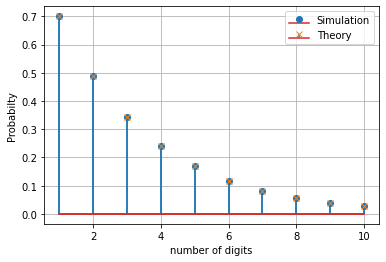
\includegraphics[width=\linewidth]{figs/3.png}
    \caption{Plot  }
    \label{3:}
\end{figure}
\item Three fair cubical dice are thrown simultaneously. The probability that all three dice have the same number of dots on the faces showing up is (up to third decimal place)...........
\solution
Let 
\begin{align}
X_{1},X_{2},X_{3} \in \{1,2,3,4,5,6\}
\end{align}
represent the three dice.

Since, all the three are fair dice, the probability of any dice showing a particular number is given by
\begin{align}
 \pr{X=i} =
    \begin{cases}
      \frac{1}{6} & \text{i=1,2,3,4,5,6}\\
       0 & \text{otherwise}
    \end{cases}       
\end{align}
If all the dice show a particular number i,
\begin{align}
\implies \pr{X_{1} =X_{2}=X_{3}=i}
\end{align}
Since the events are independent, 
\begin{multline}\label{eq1}
  \pr{X_{1} =X_{2}=X_{3}=i}\\
  =  \pr{X_{1}=i}\pr{X_{2}=i}\pr{X_{3}=i}
\end{multline}
where i=1,2,3,4,5,6.\\
There are 6 faces on a cubical dice. Hence, there are six cases in which all the dice show the same number
\begin{align}
 \pr{X_1 =X_2 =X_3}&=\sum^{6}_{i=1} \pr{X_{1} =X_{2}=X_{3}=i}
 \end{align}
 From \eqref{eq1},we have
 \begin{multline}
\pr{X_1 =X_2 =X_3}
\\=\sum^{6}_{i=1}\pr{X_{1}=i}\pr{X_{2}=i}\pr{X_{3}=i}
\end{multline}
\begin{align}
 &=\sum^{6}_{i=1}\brak{\frac{1}{6}}\brak{\frac{1}{6}}\brak{\frac{1}{6}}\\
 &=\frac{1}{36}
\end{align}

\item Candidates were asked to come to an interview with 3 pens each. Black,blue,green and red were the permitted pen colours that the candidate could bring. The probability that a candidate comes with all 3 pens having the same colour is.......

\item The probability of getting a "head" in a single toss of a biased coin is 0.3. The coin is tossed repeatedly till a "head" is obtained. If the tosses are independent, then the probability of getting "head" for the first time in the fifth toss is........
\solution
Let $X\in\mathbb{N}$ represent the number of times the experiment is performed. \\
$X=k$ represents $k-1$ failures were obtained before getting 1 success. $p$ represents the probability of success
\begin{align}
	p_X(k) &=
\begin{cases}
\brak{1-p}^{k-1}\times p & k\in \mathbb{N}\\
0 &  otherwise 
\end{cases}
\label{eq:final_result}
\end{align}
Using \eqref{eq:final_result} we get
\begin{align}
\pr{X=5}&=\brak{1-p}^{k-1}\times p\nonumber\\
&=\brak{0.7}^4\times 0.3=0.07203
\end{align}


\item Given Set A = [2,3,4,5] and Set B = [11,12,13,14,15], two numbers are randomly selected,one from each set. What is probability that the sum of the two numbers equals 16?

\begin{enumerate}
\begin{multicols}{4}
\setlength\itemsep{2em}

\item $
0.20
$
\item $
0.25
$
\item $
0.30
$
\item $
0.33
$

\end{multicols}
\end{enumerate}
\solution
Given,\\
Set A= [2,3,4,5]\\
Set B= [11,12,13,14,15]\\

Total number of element in the sample space is 20.\\

Let us define a random variable$ X \in \cbrak{0,1}$\\
\begin{table}[ht]
    \centering
    \begin{tabular}{|c|c|}
    \hline
    X=0 & the event when A+B=16\\
    \hline
    X=1 & the event when A+B $\neq$ 16\\
    \hline
    \end{tabular}
    \caption{Random Variables}
    \label{tab:Random Variables}
\end{table}

Now, probability of selecting an element from set A such that \pr{X=0} is
\begin{equation}
   \tag{7.1}
    \pr{X=0}=\pr{A+B=16}=1
\end{equation}

So,the probability of selecting an element from set B after selecting an element from set A such that \pr{X=0} is
\begin{equation}
    \tag{7.2}
    \pr{X=0}=\pr{A+B=16}= \frac{1}{5}
\end{equation}

Therefore,\\
Overall probability of randomly choosing elements from set A and set B such that \pr{X=0}is
\begin{align}
    \tag{7.3}
    \pr{X=0}&=\pr{A+B=16}\\
    \tag{7.4}
    \pr{X=0}&=1 \times \frac{1}{5}\\
    \tag{7.5}
    \pr{X=0}&= \frac{1}{5}=0.2
\end{align}


\begin{table}[ht]
    \centering
    \begin{tabular}{|c|c|c|}
    \hline
    X & 0 & 1\\
    \hline
    $\pr{X}$ & $\frac{1}{5}$ & $\frac{4}{5}$\\
    \hline
    \end{tabular}
    \caption{Probability distribution table}
    \label{tab:Probability distribution table}
\end{table}

Therefore, the correct option is (a).

\item Consider a dice with the property that the probability of a face with \textit{n} dots showing up is proportional to \textit{n}. The probability of the face with three dots showing up is......
%
\solution
Let X be random variable.\\
X $\in$ \{1,2,3,4,5,6\}\\
$p_{X}(n)\rightarrow$Probability of showing up n.\\
As $p_{X}(n)$ is proportional to n. We have,
\begin{align}
    p_{X}(n) = 
    \begin{cases}
        kn & 1 \leq n \leq 6 \\
        0  & otherwise
    \end{cases}
    \tag{8.1}
\end{align}
Where k is some real constant.

\begin{table}[ht]
\centering 
\caption{}
\begin{tabular}{|c|c|c|c|c|c|c|}
\hline
 n          & 1 & 2 & 3 & 4 & 5 & 6 \\
\hline
 $p_{X}(n)$ & k  & 2k & 3k & 4k & 5k & 6k\\
\hline
\end{tabular}
\label{8:table}
\end{table}

We know that,
\begin{align}
    \tag{8.2}
    \sum_{n=1}^6 p_{X}(n)=1
    \label{8:eq:1}
\end{align}
By substituting the values in \ref{8:eq:1}, we have
\begin{align}
    \tag{8.3}
    k+2k+3k+4k+5k+6k=1
\end{align}
\begin{align}
     \tag{8.4}
   \implies  k=\frac{1}{21}
   \label{8:eq:2}
\end{align}
Probability of the face with three dots showing up 
\begin{align}
    \tag{8.5}
    \implies p_{X}(3)=3k
\end{align}
Substituting the value of k from \ref{8:eq:2}
\begin{align}
    \tag{8.6}
    \implies p_{X}(3)=\frac{1}{7}
\end{align}

\item \textbf{Step 1.} Flip a coin twice.\\
\textbf{Step 2.} If the outcomes are (TAILS, HEADS) then output Y and stop.\\
\textbf{Step 3.} If the outcomes are either (HEADS, HEADS) or (HEADS, TAILS), then output N and stop.\\
\textbf{Step 4.} If the outcomes are (TAILS, TAILS), then go to Step 1.\\
The probability that the output of the experiment is Y is (upto two decimal places)......
%
\solution
Let flipping a coin twice be event H.\\
Sample space of event H = \cbrak{HH,HT,TH,TT}\\
Let a random variable X; $X_{i}=i$, where i=1,2,3. \\
 $X_{1}$ represents outcome \cbrak{TT}, 
 \\$X_{2}$ represents getting outcome \cbrak{TH} or output Y,
 \\ $X_{3}$ represents getting output N.\\
The state transition matrix P is shown below :
\begin{align}
\begin{array}{c c} &
\begin{array}{c c c} X_{1}  & X_{2} & X_{3} \\
\end{array}
\\
\begin{array}{c c c}
X_{1} \\
X_{2}\\
X_{3}
\end{array}
&
\left[
\begin{array}{c c c}
\frac{1}{4} & \frac{1}{4} & \frac{1}{2} \\
0 & 1 & 0 \\
0 & 0 & 1 
\end{array}
\right]
\end{array}
\end{align}
\\
\begin{figure}[h]
\caption*{\textbf{Markov chain diagram}}
\centering
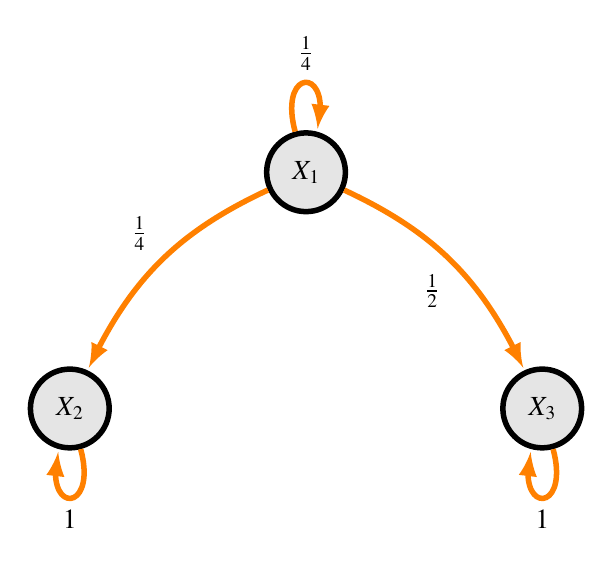
\begin{tikzpicture}
       
             % Setup the style for the states
        \tikzset{node style/.style={state, 
                                    minimum width=1cm,
                                    line width=0.7mm,
                                    fill=gray!20!white}}
        % Draw the states
        \node[node style] at (3, 0)      (bull)     {$X_{1}$};
        \node[node style] at (0, -3)      (bear)     {$X_{2}$};
        \node[node style] at (6, -3) (stagnant) {$X_{3}$};
        % Connect the states with arrows
        \draw[every loop,
              auto=right,
              line width=0.7mm,
              >=latex,
              draw=orange,
              fill=orange]
           (bull)     edge[bend left=20]            node {$\frac{1}{2}$} (stagnant)
            (bull)     edge[bend right=20] node {$\frac{1}{4}$} (bear)
            
            
            (bull) edge[loop above]             node  {$\frac{1}{4}$} (bull)
            (bear) edge[loop below]             node  {1} (bear)
            (stagnant) edge[loop below]             node  {1} (stagnant);
    \end{tikzpicture}
\end{figure}\\
From the transition matrix, we have 1 transient state and 2 absorbing states.\\ Q = $\begin{bmatrix} \frac{1}{4} \end{bmatrix}$ and R = $\begin{bmatrix} \frac{1}{4} & \frac{1}{2} \end{bmatrix}$
\begin{align}
 N ={}& \brak{I - Q}^{-1}\\
 ={}& \brak{\sbrak{1} - \sbrak{\frac{1}{4}}}^{-1}\\
 ={}& \sbrak{\frac{4}{3}}
\end{align}
We know that probability of being absorbed by state j after starting in state i is given by the $M_{i,j}$, where M = NR.\\
\begin{align}
M = \begin{bmatrix} \frac{1}{3} & \frac{2}{3} \end{bmatrix}
\end{align}.\\
 Hence the probability of being absorbed by state Y $\brak{1^{st} \text{element of R}}$ after starting with state $X_{1}\brak{1^{st}\text{element of Q}}$ is $M_{1,1}$\\
 \\
\begin{align}
\therefore \pr{Y}=\frac{1}{3}=0.33 \brak{\text{correct upto 2 decimal places}}.
\end{align}



\item Let X and Y denote the sets containing 2 and 20 distinct objects respectively and F denote the set of all possible functions defined from X and Y. Let f be randomly chosen from F. The probability of f being one-to-one is........

\item The probability that a given positive integer lying between 1 and 100 (both inclusive) is NOT divisible by 2,3 or 5 is......
\\
\solution
Let $X \in  \{1,2,...,100\}$ be the random variable representing the outcome for random selection of a number in $\{1,...,100\}$.

Since X has a uniform distribution, the probability mass function (pmf) is represented as 
\begin{align}
    \pr{X  = n} = 
    \begin{cases}
        \frac{1}{100} & 1  \le n \le 100 \\
        0 & otherwise
    \end{cases}
\end{align}
Let A represent the event that the number is divisible by 2.
Let B represent the event that the number is divisible by 3.
Let C represent the event that the number is divisible by 5.

We need to find the probability that the number is not divisible by 2, 3 or 5. Thus we need to find $1 - \pr{A+B+C}$

We know 
\begin{multline}
    \pr{A+B+C} = \pr{A} + \pr{B} + \pr{C} \\- \pr{AB} - \pr{BC} \\- \pr{AC} + \pr{ABC}\label{Shurururururururu}    
\end{multline}

\begin{table}[!ht]
\begin{center}
\begin{tabular}{|c|c|c|}
\hline
Event & Interpretation  & Probability  \\
\hline
A    & n is divisible by 2  & $\cfrac{50}{100}$ \\
B    & n is divisible by 3  & $\cfrac{33}{100}$ \\
C    & n is divisible by 5  & $\cfrac{20}{100}$ \\
AB   & n is divisible by 6  & $\cfrac{16}{100}$ \\
BC   & n is divisible by 15 & $\cfrac{6}{100}$ \\
AC   & n is divisible by 10 & $\cfrac{10}{100}$ \\
ABC  & n is divisible by 30 & $\cfrac{3}{100}$ \\
\hline
\end{tabular}
\end{center}
\caption{}
\label{gate:11}
\end{table}
%
Substituting in \eqref{Shurururururururu}, we get
\begin{multline}
    \pr{A+B+C} = \frac{50}{100} + \frac{33}{100} + \frac{20}{100} \\- \frac{16}{100} - \frac{6}{100} - \frac{10}{100} + \frac{3}{100} 
\end{multline}
Thus, 
\begin{align}
    \pr{A+B+C} = \frac{74}{100}
\end{align}
Thus required probability = 
\begin{align}
    1 - \pr{A+B+C} = \frac{26}{100}
\end{align}


\item P and Q are considering to apply for a job. The probability that P applies for the job is $\dfrac{1}{4}$, the probability that P applies for the job given that Q applies for the job is $\dfrac{1}{2}$, and the probability that Q applies for the job given that P applies for the job is $\dfrac{1}{3}$. Then the probability that P does not apply for the job given that Q does not apply for the job is 

\begin{enumerate}
\begin{multicols}{4}
\setlength\itemsep{2em}

\item $
\dfrac{4}{5}
$

\item $
\dfrac{5}{6}
$

\item $
\dfrac{7}{8}
$

\item $
\dfrac{11}{12}
$

\end{multicols}
\end{enumerate}
\solution
Let A represent the event that P applies for the job. Let B represent the event that Q applies for the job. 

According to the given information in the question,
\begin{align}
\pr{A} = \frac{1}{4} \\
\pr{A|B} = \frac{1}{2} \\
\pr{B|A} = \frac{1}{3} 
\end{align}
According to the definition of Conditional Probability,
\begin{align}
\pr{A|B} = \frac{\pr{AB}}{\pr{B}} \label{2.0.4} \\
\pr{B|A} = \frac{\pr{AB}}{\pr{A}} \label{2.0.5}
\end{align}
On substituting the values of $\pr{A}$, $\pr{B|A}$ in \eqref{2.0.5}, we get
\begin{align}
\frac{1}{3} = \frac{\pr{AB}}{\frac{1}{4}} \\
\pr{AB} = \left(\frac{1}{3} \right) \left(\frac{1}{4} \right) \\
\therefore \pr{AB} = \frac{1}{12}
\end{align}
Now substituting the values of $\pr{A|B}$, $\pr{AB}$ in \eqref{2.0.4}, we get
\begin{align}
\frac{1}{2} = \frac{\frac{1}{12}}{\pr{B}} \\
\pr{B} = \frac{\left(\frac{1}{12} \right)}{\left(\frac{1}{2} \right)} \\
\therefore \pr{B} = \frac{1}{6}
\end{align}
The probability that P does not apply for the job given that Q does not apply for the job is given by $\pr{A^{'}|B^{'}}$.

Now,
\begin{align}
A^{'}B^{'} = (A + B)^{'} \\
\Rightarrow \pr{A^{'}B^{'}} = \pr{(A + B)^{'}} \\
\therefore \pr{A^{'}B^{'}} = 1 - \pr{A + B} \label{2.0.14}
\end{align}
As we know that,
\begin{align}
\pr{A+B} = \pr{A} + \pr{B} - \pr{AB} \label{2.0.15}
\end{align}
By substituting the values of $\pr{A}$, $\pr{B}$, $\pr{AB}$ in \eqref{2.0.15}, we get
\begin{align}
\pr{A+B} = \frac{1}{4} + \frac{1}{6} - \frac{1}{12} \\
= \frac{3 + 2 - 1}{12} \\
\therefore \pr{A+B} = \frac{1}{3}
\end{align}
$\therefore$ Required Probability is 
\begin{align}
\pr{A^{'}|B^{'}} = \frac{\pr{A^{'}B^{'}}}{\pr{B^{'}}} \label{2.0.19}   
\end{align}
By substituting the values of $\pr{B}$, $\pr{A^{'}B^{'}}$ [from \eqref{2.0.14}] in \eqref{2.0.19}, we get
\begin{align}
\pr{A^{'}|B^{'}} = \frac{1 - \pr{A + B}}{1 - \pr{B}} \\
\pr{A^{'}|B^{'}} = \frac{1 - \left(\frac{1}{3} \right)}{1 - \left(\frac{1}{6} \right)} \\
\Rightarrow \pr{A^{'}|B^{'}} = \frac{\left(\frac{2}{3} \right)}{\left(\frac{5}{6} \right)} = \frac{4}{5}\\
\end{align}
$\therefore$ $\pr{A^{'}|B^{'}}$ = $\frac{4}{5}$ = 0.8

Hence, the probability that P does not apply for the job given that Q does not apply for the job is equal to $\frac{4}{5}$

$\therefore$ The correct option is (A) $\frac{4}{5}$ .



\item Two players, A and B, alternately keep rolling a fair dice. The person to get a six first wins the game. Given that player A starts the game, the probability that A wins the game is

\begin{enumerate}
\begin{multicols}{4}
\setlength\itemsep{2em}

\item $
\dfrac{5}{11}
$
\item $
\dfrac{1}{2}
$
\item $
\dfrac{7}{13}
$
\item $
\dfrac{6}{11}
$

\end{multicols}
\end{enumerate}
%
\solution
Let $X\in\{1,2,3,4,5,6\}$ be the random variable representing out come of a dice.\\
Probability of getting a six on a fair dice
\begin{align}
\Pr(X=6) &=\frac{1}{6}
\end{align}
Probability of not getting a six on a fair dice
\begin{align}
\Pr(X\neq6)=\frac{5}{6}
\end{align}
The probability of some one wining in their $n^{th}$ trail is
    \begin{multline}
        \Pr{(X_n=6|X_k\neq6,k=1,2,3...,n-1)}\\
    =\frac{1}{6}\brak{\frac{5}{6}}^{n-1}
    \end{multline}
Let the probability of a wining the game is $\Pr{(A)}$\\
If A start's the game then A can win on odd numbered trail$(n)$\\
\begin{align}
n&=2m+1
\end{align}
Inorder for A to win B must lose in all of it's trails until A gets a six.\\
Therefore,
\begin{align}
   \Pr{(A)}&=\Pr{(X_1=6)}+\Pr{(X_3=6)}+\Pr{(X_5=6)}+....\\
    \Pr{(A)}&=\brak{\frac{1}{6}}+\brak{\frac{1}{6}\brak{\frac{5}{6}}^{2}}+\brak{\frac{1}{6}\brak{\frac{5}{6}}^{4}}...\\
    &=\frac{1}{6}\sum_{m=0}^{\infty}\brak{\frac{5}{6}}^{2m}\\
    &=\frac{\frac{1}{6}}{1-\brak{\frac{5}{6}}^2}\\
    &=\frac{6}{11}\\
    \implies \Pr{(A)}&=\frac{6}{11}
\end{align}
Therefore, The probability that A wins the game=$\Pr{(A)=\frac{6}{11}}$

\item A continuous random variable X has a probability density function $f(x) = e^{-x}, 0<x<\infty$. Then $P(X>1)$ is
\begin{enumerate}
\begin{multicols}{4}
\setlength\itemsep{2em}

\item $0.368$
\item $0.5$
\item $0.632$
\item $1.0$

\end{multicols}
\end{enumerate}
%
\solution
We know that,
\begin{align}
\int_{-\infty}^{\infty}{f_x(x)}\,dx = 1.\\
\int_{-\infty}^{0}{f_x(x)}\,dx +\int_{0}^{\infty}{f_x(x)}\,dx = 1\label{ee2016-33:eq_(1)}\\
\int_{-\infty}^{0}{ae^{4x}}\,dx +\int_{0}^{\infty}{\frac{3}{2}e^{-3x}}\,dx = 1\label{ee2016-33:eq_(2)}
\end{align}
The expression \eqref{ee2016-33:eq_(2)} was written from \eqref{ee2016-33:eq_(1)} since,
\begin{align*}
  u(x) = 
  \begin{cases}
  1, & \text{for } x \geq 0\\
  0, & \text{otherwise } 
  \end{cases}
\end{align*}

Simplifying \eqref{ee2016-33:eq_(2)} we have:
\begin{align}
\int_{-\infty}^{0}{ae^{4x}}\,dx +\int_{0}^{\infty}{\frac{3}{2}e^{-3x}}\,dx = 1\nonumber\\
\implies a\left[\frac{e^{4x}}{4}\right]_{-\infty}^{0} +    \frac{3}{2}\left[\frac{e^{-3x}}{-3}\right]_0^{\infty} = 1\\
\implies a\left[\frac{1}{4}-0\right] - \frac{1}{2}\left[0-1\right] = 1\\
\implies \frac{a}{4} + \frac{1}{2} =1 \implies a = 2
\end{align}
Therefore,
\begin{align}
 f_x(x) = 
  \begin{cases}
  \frac{3}{2}e^{-3x}, & \text{for } x \geq 0\\
  2e^{4x}, & \text{for } x < 0
  \end{cases}
\end{align}

The plot for PDF of $X$ can be observed at figure \ref{ee2016-33:fig:The PDF of X}
\begin{figure}[!ht]
       \centering
    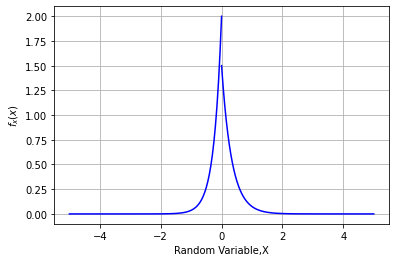
\includegraphics[width=.9\columnwidth] {solutions/ee/2016/33/Assignment_2_Fig_2.png}
    \caption{The PDF of X}
    \label{ee2016-33:fig:The PDF of X}
\end{figure}

The CDF of X is defined as follows:
\begin{align}
    F_X(x)= \pr{X\leq x}
\end{align}
Now for $x<0$,
\begin{align}
\pr{X\leq x} &= \int_{-\infty}^{x}{f_x(x)}\,dx\\
&= \int_{-\infty}^{x}{2e^{4x}}\,dx\\
&= 2\left[\frac{e^{4x}}{4}\right]_{-\infty}^{x}\\
&= 2\left[\frac{e^{4x}}{4}-0\right]\\
&= \frac{e^{4x}}{2}
\end{align}
Similarly for $x\geq0$,
\begin{align}
\pr{X\leq x} &= \int_{-\infty}^{x}{f_x(x)}\,dx\\
&= \int_{-\infty}^{0}{2e^{4x}}\,dx +\int_{0}^{x}{\frac{3}{2}e^{-3x}}\,dx\\
&= 2\left[\frac{e^{4x}}{4}\right]_{-\infty}^{0}+\left[\frac{-e^{-3x}}{2}\right]_{0}^{x}\\
&= 2\left[\frac{1}{4}-0\right]-\frac{1}{2}\left[e^{-3x}-1\right]\\
&= 1-\frac{e^{-3x}}{2}
\end{align}

The CDF of X is as below:
\begin{align}
 F_X(x) = 
  \begin{cases}
  1-\frac{e^{-3x}}{2}, & \text{for } x \geq 0\\
  \frac{e^{4x}}{2}, & \text{for } x < 0
  \end{cases}
\end{align}

The plot for CDF of $X$ can be observed at figure \ref{ee2016-33:fig:The PDF of X}.
\begin{figure}[!ht]
       \centering
    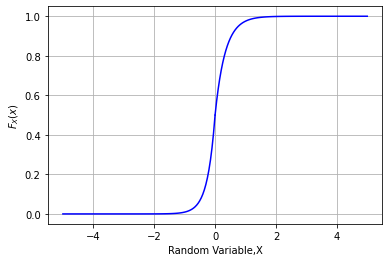
\includegraphics[width=.9\columnwidth] {solutions/ee/2016/33/Assignment_2_Fig_1.png}
    \caption{The CDF of X}
    \label{ee2016-33:fig:The CDF of X}
\end{figure}

\begin{align}
\therefore
\pr{X\leq0} = F_X(0)=\frac{1}{2}
\end{align}




\item A random variable X has probability density function $f(x)$ as given below:\\
\begin{align}
f(x) =
\begin{cases}
a+bx
&  0<x<1
\\      
0
& \text{otherwise}
\end{cases}
\label{a}
\end{align}
\\
If the expected value $E[X]=\dfrac{2}{3}$, then $Pr[X<0.5]$ is..........
\\
\solution

We know that the total probability is one,
\begin{equation}
    \int_{-\infty}^{\infty}{f\brak{x} dx} = 1\label{b}
\end{equation}
Using \eqref{a} in \eqref{b},
\begin{align}
    \int_{0}^{1}{(a+bx)\,dx} = 1\\
    \sbrak{ax+\frac{bx^2}{2}}_0^1=1\\
    \left(a+\frac{b}{2}\right)-0=1\\
    \implies a+\frac{b}{2}=1 \label{c}
\end{align}
We know that expectation value of X,
\begin{align}
    E\brak{X}=\int_{-\infty}^{\infty}xf\brak{x}\,dx\label{d}
\end{align}
%
Using $E\brak{X}=\frac{2}{3}$ and \eqref{a} in \eqref{d}, we get
\begin{align}
     \frac{2}{3}&=\int_{0}^{1}x(a+bx)\,dx\\
     &=\int_{0}^{1} ax+bx^2\,dx\\
     &= \sbrak{\frac{ax^2}{2}+\frac{bx^3}{3}}_0^1\\
     &= \frac{a}{2}+\frac{b}{3}-0\\
     \implies\frac{a}{2}+\frac{b}{3}&=\frac{2}{3}\label{e}
\end{align}
By solving \eqref{c} and \eqref{e}, we get 
\begin{align}
    a\, =\, 0 \,\,and\,\, b\, =\, 2.
\end{align}
Using values of $a$ and $b$ in \eqref{a}, we get
\begin{align}
f\brak{x}
= 
\begin{cases}
2x & 0<x<1
\\
0 & otherwise\label{f}\\
\end{cases}
\end{align}
\begin{figure}[ht]
    \centering
    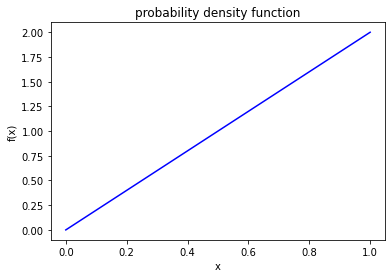
\includegraphics[width=\columnwidth]{solutions/ec/15/figures/assign2.png}
    \caption{Probability Density Function (PDF) of X}
    \label{Figure_1}
\end{figure}
The graph of PDF of X is \ref{Figure_1}
\par Let $F_X(x)$ be the cumulative distribution function of random variable X.
\begin{align}
    F_X(x)=\int_{-\infty}^x f\brak{x} dx\label{x}
\end{align}
$F_X(x)$ can be obtained from the uniform distribution of a random variable U on (0,1) and let U=$X^2$. 
\begin{align}
    0 < U < 1
\end{align}
As for random variable X also,
\begin{align}
    0 < F_X(x) < 1
\end{align}
This similarity between U and $F_X(x)$ is used to generate the random variable X from U.
\begin{align}
    F_X(x)&= \pr{X<x}\\
    &=\pr{\sqrt{U}<x}\\
    &=\pr{U<x^2}\\
    &=F_U(x^2)\label{y}
\end{align}
From uniform distribution,
\\The graph of Probability Density Function (PDF) of U is \ref{Figure_2}
\begin{figure}[ht]
    \centering
    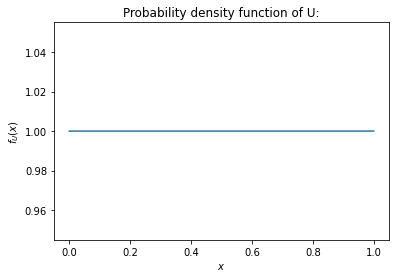
\includegraphics[width=\columnwidth]{solutions/ec/15/figures/assign2_2.png}
    \caption{Probability Density Function (PDF) of U}
    \label{Figure_2}
\end{figure}
\begin{align}
    F_U(x)=
    \begin{cases}
0 & x\leq0\\
x & 0<x<1
\\
1 & x\geq1\label{z}\\
\end{cases}
\end{align}
\begin{figure}[ht]
    \centering
    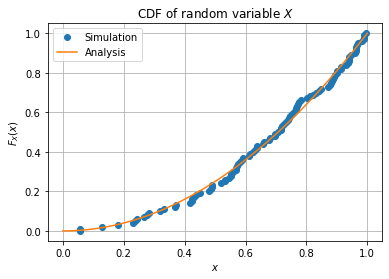
\includegraphics[width=\columnwidth]{solutions/ec/15/figures/assign2_1.png}
    \caption{Cumulative Density Function (CDF)}
    \label{Figure_3}
\end{figure}
\\Using \eqref{z} in \eqref{y},
\\Cumulative distribution function (CDF) of random variable X is,
\begin{align}
F_X(x)= \pr{X<x}
= 
\begin{cases}
0 & x\leq0\\
x^2 & 0<x<1
\\
1 & x\geq1\label{g}\\
\end{cases}
\end{align}
The graph of Cumulative distribution function (CDF) of random variable X is \ref{Figure_3}\\
Now we have to find \pr{X<0.5},Using  \eqref{g},
\begin{align}
    \pr{X<0.5} &= (0.5)^2\\
  \implies \pr{X<0.5} &= 0.25
\end{align}




\item Two independent random variables X and Y are uniformly distributed in the interval $[-1,1]$.The probability that max$[X,Y]$ is less than $\dfrac{1}{2}$ is

\begin{enumerate}
\begin{multicols}{4}
\setlength\itemsep{2em}

\item $
\dfrac{3}{4}
$
\item $
\dfrac{9}{16}
$
\item $
\dfrac{1}{4}
$
\item $
\dfrac{2}{3}
$
\end{multicols}
\end{enumerate}

\item The input X to the binary Symmetric Channel (BSC) shown in Fig. \ref{fig:7} is '1' with probability 0.8. The cross-over probability is $\dfrac{1}{7}$. If the received bit Y=0, the conditional probability that '1' was transmitted is........\\


\begin{figure}[!h]
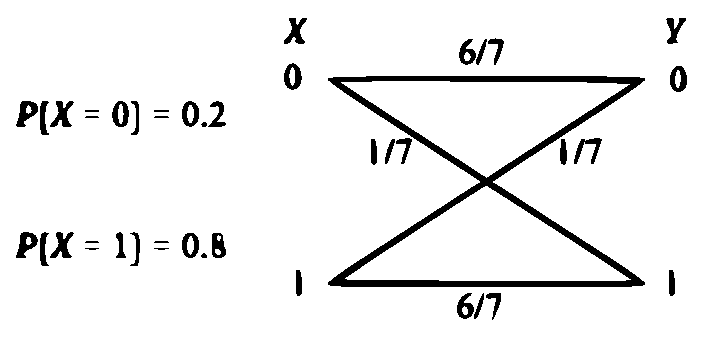
\includegraphics[width=\columnwidth]{./figs/figure7.eps}
\caption{}
\label{fig:7}
\end{figure}
%
\solution
\begin{align}
    \pr{X = 1|Y = 0}&=\frac{\pr{\{X=1\}\{Y=0\}}}{\pr{Y=0}} \label{eq:1}\\
    \pr{Y = 0|X = 1}&=\frac{\pr{\{X=1\}\{Y=0\}}}{\pr{X=1}} \label{eq:2}
\end{align}
From \eqref{eq:2},
\begin{align}
    \pr{\{X=1\}\{Y=0\}} &= \pr{Y = 0|X = 1}\pr{X=1} \label{eq:3}
\end{align}
Substituting \eqref{eq:3} in \eqref{eq:1},
\begin{align}
    \pr{X = 1|Y = 0} &= \frac{\pr{Y = 0|X = 1}\pr{X=1}}{\pr{Y=0}} \label{eq:7}
\end{align}
Given data,
\begin{align}
    \pr{Y = 0|X = 1} =\frac{1}{7}, \pr{Y =0|X=0}=\frac{6}{7} \label{eq:4}
\end{align}
\begin{multline}
    \pr{Y=0} = \pr{Y = 0|X = 1}\pr{X=1} +\\ \pr{Y = 0|X = 0}\pr{X=0} \label{eq:6}
\end{multline}
Substituting the values from \eqref{eq:4} and the data given in the question in \eqref{eq:6},
\begin{align}
    \pr{Y=0} &= \frac{2}{7} \label{eq:5}
\end{align}
Substituting \eqref{eq:4}, \eqref{eq:5} and the data given in the question in \eqref{eq:7},
\begin{align}
    \pr{X = 1|Y = 0} = 0.4
\end{align}



\item A fair coin is tossed till a head appears for the first time. The probability that the number of requried tosses is odd,is
\begin{enumerate}
\begin{multicols}{4}
\setlength\itemsep{2em}
\item $
\dfrac{1}{3}
$
\item $
\dfrac{1}{2}
$
\item $
\dfrac{2}{3}
$
\item $
\dfrac{3}{4}
$
\end{multicols}
\end{enumerate}

\item A box contains 4 white balls and 3 red balls. In succession, two balls are randomly selected and removed from the box. Given that the first removed ball is white, the probability that the second removed ball is red is
\begin{enumerate}
\begin{multicols}{4}
\setlength\itemsep{2em}
\item $
\dfrac{1}{3}
$
\item $
\dfrac{3}{7}
$
\item $
\dfrac{1}{2}
$
\item $
\dfrac{4}{7}
$

\end{multicols}
\end{enumerate}
\solution
Consider, Bernoulli random variables Say $X_1$ and $X_2$. Required probability is 
\begin{align}
Pr(X_2=0|X_1=1) = \frac{Pr(X_1=1, X_2=0)}{Pr(X_1=1)}\\
= \frac{\frac{2}{7}}{\frac{4}{7}}=\frac{1}{2}
=\frac{1}{2}
\end{align}
Hence $(\mathrm{C})$ is correct option.
\item Let X be a random variable with a probability density function
\begin{align}
f(x) = 
\begin{cases}
0.2 & \abs{x}\leq1
\\
0.1 & 1\leq\abs{x}\leq4
\\
0 & otherwise
\end{cases}
\label{pdf}
\end{align}

Find $\pr{0.5< X \leq 5}$
\\
\solution

We know, if X is a continuous random variable, and its p.d.f is given by $f(x)$, then we define the c.d.f $F(x)$ as:
\begin{align}
F(x) = \pr{X \leq x} 
\label{formula1}
\end{align}
and is given by:
\begin{align}
F(x) = \int_{-\infty}^{x}f(x)\,dx 
\label{formula2}
\end{align}

$f(x)$ is a valid p.d.f because: 
\begin{enumerate}
    \item The area under the curve of the p.d.f is 1, i.e:
    \begin{align}
        \int_{-\infty}^{\infty} f(x)\,dx = 1
    \end{align}
    \item $f(x) \geq 0$ for all $x \in \mathbb{R}$\\
\end{enumerate}
Since $f(x)$ is a valid p.d.f, from \eqref{formula2}, we get the following c.d.f:
\begin{align}
F(x) = 
\begin{cases}
0 & x \leq -4
\\
0.1(x + 4) & -4\leq x\leq -1
\\
0.3 + 0.2(x+1) & -1 \leq x \leq 1
\\
0.7 + 0.1(x-1) & 1 \leq x \leq 4
\\
1 & 4 \leq x
\end{cases}
\label{cdf}
\end{align}


    Thus,
    \begin{multline}
    \pr{0.5 \leq X \leq 5} \\ =F(5) - F(0.5) = 0.4
    \end{multline}

\begin{figure}[!ht]
\centering
 \includegraphics[width=\columnwidth]{solutions/ec/20/figures/graph_pdf.png}
 \caption{plot of $f(x)$- p.d.f}
     \includegraphics[width=\columnwidth]{solutions/ec/20/figures/graph_cdf.png}
     \caption{plot of $F(x)$- c.d.f}
 \end{figure}

% The p.d.f is shown below:\\
%  \includegraphics[width=\linewidth]{figures/graph_pdf.png}
% The c.d.f is shown below:\\
%  \includegraphics[width=\linewidth]{figures/graph_cdf.png}



\item Consider two identically distributed zero-mean random variables U and V. Let the cumulative distribution functions of U and 2V be F(\textit{x}) and G(\textit{x}) respectively. Then,for all values of \textit{x}
\begin{enumerate}
\begin{multicols}{2}
\setlength\itemsep{2em}
{\small
\item $
F(x)-G(x)\leqslant0
$
\item $
F(x)-G(x)\geqslant0
$
\item $
(F(x)-G(x))\textit{x}\leqslant0
$
\item $
(F(x)-G(x))\textit{x}\geqslant0
$
}
\end{multicols}
\end{enumerate}
%
\solution
If $X$ is a random variable, the cumulative distribution functions of U and 2V can be written in terms of $X$ as
\begin{align} \label{equation-1}
    F(x)=\pr{X \leq x} 
\end{align}
\begin{align}
    G(x)=\pr{2X \leq x}
\end{align}
Or,
\begin{align} \label{equation-2}
     G(x)=\pr{X \leq x/2}
\end{align}
Using \ref{equation-1} in \ref{equation-2}, we can see that
\begin{align} \label{equation-3}
    G(x)=F(x/2)
\end{align}
So,
\begin{align}
    F(x)-G(x)=F(x)-F(x/2)
\end{align}
As F is Cumulative Distribution Function, it is non-decreasing.\\
That means for $x \geq y$, $F(x) \geq F(y)$.\\ \\
Using this, we can form the following table:
\begin{table}[h!]
    \centering
    \begin{tabular}{|c|c|c|}
        \hline
        Case & $F(x)-F(x/2)$ & $(F(x)-F(x/2))x$ \\
        \hline
        $x \geq 0$ & $\geq 0$ & $\geq 0$ \\
        \hline
        $x \leq 0$ & $\leq 0$ & $\geq 0$ \\
        \hline
    \end{tabular}
    \caption{}
    \label{table-1}
\end{table}\\
From the table we can see that for any value of $x$,
\begin{align}
    (F(x)-F(x/2))x \geq 0
\end{align}
Or, using \ref{equation-3},
\begin{align}
    (F(x)-G(x))x \geq x
\end{align}
%\item Let U and V be two independent and identically distributed random variables such that $
%P(U=+1)=P(U=-1)=\dfrac{1}{2}.
%$
%The entropy H(U+V) in bits is
%
%\begin{enumerate}
%\begin{multicols}{4}
%\setlength\itemsep{2em}
%\item $
%\dfrac{3}{4}
%$
%\item 1
%\item $
%\dfrac{3}{2}
%$
%\item $\log_23
%$

%\end{multicols}
%\end{enumerate}

\item Let U and V be two independent zero mean Gaussian random variables of variances $\dfrac{1}{4}$ and $\dfrac{1}{9}$ respectively. The probability $P(3V\geqslant2U)$ is
\begin{enumerate}
\begin{multicols}{4}
\setlength\itemsep{2em}
\item $
\dfrac{4}{9}
$
\item $
\dfrac{1}{2}
$
\item $
\dfrac{2}{3}
$
\item $
\dfrac{5}{9}
$
\end{multicols}
\end{enumerate}

\item Two independent random variables X and Y are uniformly distributed in the interval $[-1,1]$. The probability that max $[X,Y]$ is less than $\dfrac{1}{2}$ is
\begin{enumerate}
\begin{multicols}{4}
\setlength\itemsep{2em}
\item $
\dfrac{3}{4}
$
\item $
\dfrac{9}{16}
$
\item $
\dfrac{1}{4}
$
\item $
\dfrac{2}{3}
$
\end{multicols}
\end{enumerate}

\item A binary symmetric channel (BSC) has a transition probability of $\dfrac{1}{8}$. If the binary transmit symbol X is such that $P(X=0)=\dfrac{9}{10}$, then the probability of error for an optimum receiver will be
\begin{enumerate}
\begin{multicols}{4}
\setlength\itemsep{2em}
\item $
\dfrac{7}{80}
$
\item $
\dfrac{63}{80}
$
\item $
\dfrac{9}{10}
$
\item $
\dfrac{1}{10}
$
\end{multicols}
\end{enumerate}
\solution

\begin{figure}[h!]
\centering
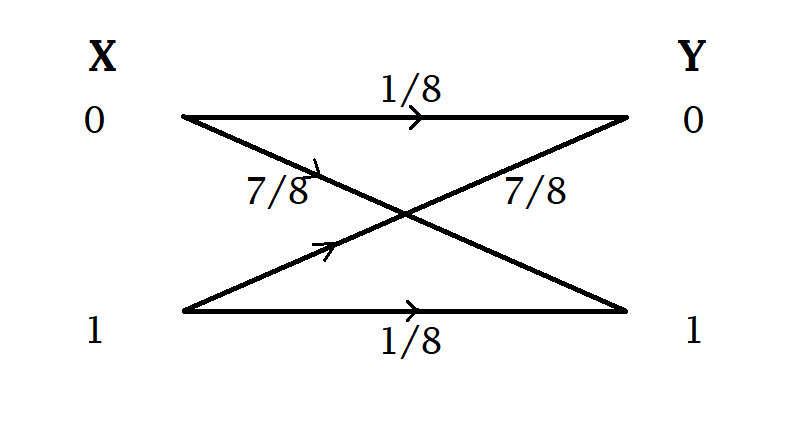
\includegraphics[width=\columnwidth]{solutions/24/Figure.png}
\caption{Binary symmetric channel}
\label{fig:BSC}
\end{figure}

Let random variables, $X \in \{0,1\}$ denote the bit transmitted and $Y \in \{0,1\}$ denote the output bit received.
\\From the given information, 
\begin{align}
    \pr{X=0} = \frac{9}{10}\\
    \pr{X=1} = 1-\pr{X=0} = \frac{1}{10}
\end{align}
Also given, transition probability = $\frac{1}{8}$. Transition probability is the probability with which the bit is transmitted correctly. That gives, 
\begin{align}
    \pr{Y=1|X=1}=\pr{Y=0|X=0}=\frac{1}{8}
\end{align}
\begin{multline}
\text{Probability that the bit is not transmitted correctly}  \\
= 1-\text{transition probability}\\
= 1-\frac{1}{8} = \frac{7}{8}
\end{multline}
That gives,
\begin{align}
    \pr{Y=0|X=1}=\pr{Y=1|X=0}=\frac{7}{8}
\end{align}
Let E denote the event that bit is transmitted incorrectly. Probability of error, $\pr{E}$
\begin{multline}
    \pr{E} = \pr{X=0}\pr{Y=1|X=0}\\ + \pr{X=1}\pr{Y=0|X=1}
\end{multline}
On substituting the values,
\begin{align}
    \pr{E} & = \frac{9}{10}\times\frac{7}{8} + \frac{1}{10}\times\frac{7}{8} \\
    & = \frac{63}{80} + \frac{7}{80}\\
    & = \frac{7}{8}
\end{align}
\rightline{Answer: No option matches}



\item A fair coin is tossed till a head appears for the first time. The probability that the number of requried tosses is odd,is
\begin{enumerate}
\begin{multicols}{4}
\setlength\itemsep{2em}
\item $
\dfrac{1}{3}
$
\item $
\dfrac{1}{2}
$
\item $
\dfrac{2}{3}
$
\item $
\dfrac{3}{4}
$
\end{multicols}
\end{enumerate}
\solution
We can see that if the first toss is guaranteed to be a head, then the problem is reduced to finding the probability of getting one head in 2 coin tosses, since all the 3 trials are independent.
Let $K=\{0, 1, 2\}$ be the random variable denoting the number of heads obtained in 2 tosses of a fair coin. The event can be represented by a binomial distribution b(n,p).
In binomial distribution b(n,p), 
\begin{align}
Pr\brak{K=i}= \binom{n}{i}p^i \cdot (1-p)^{n-i}.
\end{align}
Here $n=2, p=0.5$.
 We can see that the probability of $K=1$ is 
 \begin{align}
 Pr\brak{K=1}&=\binom{2}{1} \cdot 0.5^2\\
 &=\frac{1}{2}
 \end{align}
 
From $\brak{2.0.1}$ and $\brak{2.0.2}$, we see that probability of getting exactly 2 heads in 3 tosses, if the first toss is a head, is 0.5.

%\item A BPSK scheme operating over an AWGN channel with noise power spectral density of $\dfrac{N_0}{2}$, uses equiprobable signals $
%s_1(t) = {\sqrt{\frac{2E}{T}}} \sin (\omega_ct)
%$ and $
%s_2(t) = {\sqrt{\frac{2E}{T}}} \sin (\omega_ct)
%$
%over the symbol interval $(0,T)$. If the local oscillator in a coherent receiver is ahead in phase by $45\degree$ with respect to the received signal, the probability of error in the resulting system is
%\begin{enumerate}
%\begin{multicols}{4}
%\setlength\itemsep{2em}
%\item $
%Q\bigg(\sqrt{\dfrac{2E}{N_0}}\bigg)
%$
%\item $
%Q\bigg(\sqrt{\dfrac{E}{N_0}}\bigg)
%$
%\item $
%Q\bigg(\sqrt{\dfrac{E}{2N_0}}\bigg)$
%\item $
%Q\bigg(\sqrt{\dfrac{E}{4N_0}}\bigg)$
%
%\end{multicols}
%\end{enumerate}

\item A fair dice is tossed two times. The probability that the second toss result in a value that is higher than the first toss is
\begin{enumerate}
\begin{multicols}{4}
\setlength\itemsep{2em}
\item $
\dfrac{2}{36}
$
\item $
\dfrac{2}{6}
$
\item $
\dfrac{5}{12}
$
\item $
\dfrac{1}{2}
$
\end{multicols}
\end{enumerate}
%
\solution
Given, a fair die, which is tossed twice. Let the random variable $X_{i}\in\{1,2,3,4,5,6\},i=1,2,$ represent the outcome of the number on the die in the first, second toss respectively.  
The probability  mass function (PMF) for a fair die is expressed as \begin{align}
    \tag{26.1}
    \label{eq:pmf}
    p_{X_{i}}(n)=\Pr(X_{i}=n) = 
	\begin{cases}
	\dfrac{1}{6}, & 1\leq n\leq6 \\~\\[-1em]
	0, & otherwise
	\end{cases}
\end{align}
Using \eqref{eq:pmf}, the cumulative distribution function (CDF) is obtained to be
\begin{align}
    \tag{26.2}
    F_{X_{i}}(r)=\Pr(X_{i}\leq r) = 
	\begin{cases}
	\dfrac{r}{6}, & 1\leq r\leq6 \\~\\[-1em]
	1, & r \geq 7 \\~\\[-1em]
	0, & otherwise
	\end{cases}
	\label{eq:26.2}
\end{align}
\begin{align}
    \tag{26.3}
    X_{1}<X_{2}\Rightarrow X_{2}=k,X_{1}\leq k-1
\end{align}
$\because X_{1},X_{2}$ are independent,
\begin{align}
    \tag{26.4}
    Pr(X_{1}<X_{2})=E\left[F_{X_{1}}(X_{2}-1)\right]
    \label{eq:probeqn}
\end{align}
After unconditioning \eqref{eq:probeqn}, we get
\begin{align}
    \tag{26.5}
    Pr(X_{1}<X_{2})=\sum_{k=1}^{6}p_{X_{2}}(k) F_{X_{1}}(k-1)
\end{align}
Substituting \eqref{eq:pmf} and \eqref{eq:26.2}, we get
\begin{align}
    \tag{26.6}
    Pr(X_{1}<X_{2})=\sum_{k=1}^{6}\dfrac{1}{6}\left(\dfrac{k-1}{6} \right)
\end{align}
On solving, we get
\begin{align}
    \tag{26.7}
    Pr(X_{1}<X_{2})=\dfrac{5}{12}\text{(option (C))}
\end{align}
\begin{table}[h!]
\centering
\caption{Cases and their theoretical probabilities}
\label{table:1}
\begin{tabular}{|c||c|c|c|}
    \hline
    Case & $X_{1}<X_{2}$& $X_{1}>X_{2}$& $X_{1}=X_{2}$ \\
    \hline
    %& & &\\
    Probability & $\dfrac{5}{12}$ & $\dfrac{5}{12}$ & $\dfrac{1}{6}$\\[1ex]
    \hline
\end{tabular}
\end{table}
\item A fair coin is tossed 10 times. What is the probability that ONLY the first two tosses will yield heads?
\begin{enumerate}
\begin{multicols}{2}
\setlength\itemsep{1em}
{\small
\item $
\brak{\frac{1}{2}}^2
$
\item $
{\comb{10}{2}}\brak{\frac{1}{2}}^2
$
\item $
\brak{\frac{1}{2}}^{10}
$
\item $
{\comb{10}{2}}\brak{\frac{1}{2}}^{10}
$
}
\end{multicols}
\end{enumerate}
%
\solution
Let $M \sim B\brak{n,h}$ be a random variable representing number of 'heads' in 10 tosses.
So M has a binomial distribution :
\begin{align}
    \pr{M=k} = \comb{n}{k} \times (h)^{n-k} \times (t)^{k}\label{0.0.1}
\end{align}
Where
\begin{itemize}
    \item n = Total number of tosses = 10
    \item h = Probability that 'head' appears in a toss = \( \frac{1}{2} \)
    \item t = Probability that 'tail' appears in a toss = \( \frac{1}{2} \)
\end{itemize}
\bigskip
So,
\begin{align}
    \pr{M=k} = \comb{10}{k} \times \brak{\frac{1}{2}}^{10-k} \times \brak{\frac{1}{2}}^{k}\label{0.0.2}
\end{align}
\begin{table}[!ht]
    \begin{center}
        \small
        \resizebox{\columnwidth}{!}
        {
            \begin{tabular}{|c|c|}
                \hline
                n            & 10                                                                            \\
                \hline
                $\pr{M = 2}$ & $\comb{10}{2} \times \brak{\frac{1}{2}}^{10-2} \times \brak{\frac{1}{2}}^{2}$ \\
                \hline
                Calculation  & $\comb{10}{2} \times \brak{\frac{1}{2}}^{10}$                                 \\
                \hline
                Value        & 0.043945                                                                      \\
                \hline
            \end{tabular}
        }
    \end{center}
\end{table}
\begin{itemize}
    \item Number of ways of choosing 2 positions from 10 tosses = $\comb{10}{2}$
          \bigskip
    \item Number of favourable outcome = 1 (Choosing FIRST and SECOND tosses as heads)
          \bigskip
    \item Probability that chosen 2 'heads' are from FIRST and SECOND tosses = \(\displaystyle \frac{1}{\comb{10}{2}}\)
          \bigskip
\end{itemize}
Probability that ONLY the first 2 tosses yield heads
\begin{align}
    = & \pr{M = 2} \times \displaystyle \frac{1}{\comb{10}{2}}                    \\
    = & \comb{10}{2} \times \brak{\frac{1}{2}}^{10} \times \frac{1}{\comb{10}{2}} \\
    = & \brak{\frac{1}{2}}^{10}
\end{align}
\item Consider two independent random variables X and Y with identical distributions. The variables X and Y take value 0, 1 and 2 with probabilities $\dfrac{1}{2}$, $\dfrac{1}{4}$ and $\dfrac{1}{4}$ rrespectively. What is the conditional probability $P(X+Y = 2|X-Y =0)$?

\begin{enumerate}
\begin{multicols}{4}
\setlength\itemsep{2em}

\item 0
\item $\dfrac{1}{16}$
\item $\dfrac{1}{6}$
\item 1

\end{multicols}
\end{enumerate}
%
\solution
The values that the random variable X can take along with its probabilities are given by
\begin{table}[h]
\centering
\begin{tabular}{|l|l|l|l|}
\hline
X             & 0             & 1             & 2             \\ \hline
$\Pr\brak{X}$ & $\frac{1}{2}$ & $\frac{1}{4}$ & $\frac{1}{4}$ \\ \hline
\end{tabular}
\end{table}
\newline
The values that the random variable Y can take along with its probabilities are given by
\begin{table}[h]
\centering
\begin{tabular}{|l|l|l|l|}
\hline
Y             & 0             & 1             & 2             \\ \hline
$\Pr\brak{Y}$ & $\frac{1}{2}$ & $\frac{1}{4}$ & $\frac{1}{4}$ \\ \hline
\end{tabular}
\end{table}
\begin{align}
\Pr\brak{X-Y=0}=\frac{1}{2}\times\frac{1}{2}+\frac{1}{4}\times\frac{1}{4}+\frac{1}{4}\times\frac{1}{4}=\frac{6}{16}\\
\Pr\brak{(X+Y=2),(X-Y=0)}=\frac{1}{4}\times\frac{1}{4}=\frac{1}{16}
\end{align}
\begin{align}
\Pr\brak{X+Y=2\:|\:X-Y=0}\notag\\
=&\frac{\Pr\brak{(X+Y=2),(X-Y=0)}}{\Pr\brak{X-Y=0}}\notag\\
=&\frac{\frac{1}{16}}{\frac{6}{16}}=\frac{1}{6}
\end{align}

\item A discrete random variable X takes values from 1 to 5 with probabilities as shown in the table. A student calculates the mean of X as 3.5 and her teacher calculates the variance of X as 1.5. Which of the following statements is true?

\begin{center}
\begin{tabular}{|c|c|c|c|c|c|}\hline

k & 1 & 2 & 3 & 4 & 5\\ \hline
P(X=k) & 0.1 & 0.2 & 0.4 & 0.2 & 0.1\\ \hline
\end{tabular}
\end{center}

\begin{enumerate}
\item Both the student and the teacher are right
\item Both the student and the teacher are wrong
\item The student is wrong but the teacher is right
\item The student is right but the teacher is wrong
\end{enumerate}

%\item A communication channel with AWGN operating at a signal to noise $SNR\gg1$ and bandwidth B has capacity $C_1$. If the SNR is doubled keeping B constant, the resultant capacity $C_2$ is given by
%
%\begin{enumerate}
%\begin{multicols}{4}
%\setlength\itemsep{2em}
%
%\item $
%C_2 \approx 2C_1
%$
%\item $
%C_2 \approx C_1 + B
%$
%\item $
%C_2 \approx C_1 + 2B
%$
%\item $
%C_2 \approx C_1 + 0.3B
%$
%\end{multicols}
%\end{enumerate}

\item If E denotes expectation, the variance of a random variable X is given by
\begin{enumerate}
\begin{multicols}{2}
\setlength\itemsep{2em}
\item $
E[X^2]-E^2[X]
$
\item $
E[X^2]+E^2[X]
$
\item $
E[X^2]
$
\item $
E^2[X]
$
\end{multicols}
\end{enumerate}
%
\solution
Before we start the proof we need to know 3 properties of expectation
\begin{equation}
E[f\brak{x}+g\brak{x}] = E[f\brak{x}]+E[g\brak{x}]
\end{equation}
If $k$ is a constant value then 
\begin{align}
E[k\cdot g\brak{x}] &= k\cdot E[g\brak{x}]\\
E[k]&=k
\end{align}
Now variance of random $X$ is given by 
\begin{align}
\nonumber \nonumber Var\brak{X} &= E[\brak{X-\mu}^2] \quad \text{where} \: \mu =E[X]\\
\nonumber \\
\nonumber Var\brak{X}&= E[X^2-2\mu\cdot X + \mu^2]\\
\nonumber\\
\nonumber &= E[X^2]-E[2\mu\cdot X] + E[\mu^2] \:\: \text{from } \brak{1}\\
\nonumber\\
\nonumber &=E[X^2]-2\mu\cdot E[X] + \mu^2 \:\: \text{from} \brak{2} \text{and} \brak{3}\\
\nonumber \\
\nonumber &=E[X^2]-2\mu^2+\mu^2 \quad \brak{\because E[X]=\mu}\\
\nonumber \\
\nonumber &= E[X^2]-\mu^2\\
\nonumber \\
\nonumber &= E[X^2]-E^2[X] \quad \brak{\because \: \mu = E[X]}
\end{align}


\item An examination consists of two papers, Paper 1 and Paper 2. The probability of failing in Paper 1 is 0.3 and that in Paper 2 is 0.2. Given that a student has failed in Paper 2, the probability of failing in Paper 1 is 0.6. The probability  of a student failing in both the papers is:
\begin{enumerate}
\begin{multicols}{4}
\setlength\itemsep{2em}
\item 0.5
\item 0.18
\item 0.12
\item 0.06

\end{multicols}
\end{enumerate}
%
\solution
\input{solutions/ec/31.tex}

\item A probability density function is of the form\\
{\centering $p(\textit{x}) = Ke^{-\alpha |x|}, \textit{x}\in(-\infty,\infty)$\\}
The value of K is 

\begin{enumerate}
\begin{multicols}{4}
\setlength\itemsep{2em}

\item 0.5
\item 1
\item $0.5\alpha$
\item $\alpha$

\end{multicols}
\end{enumerate}

\item Consider a binary digital communication system with equally likely 0's and 1's. When binary 0 is transmitted the voltage at the detector input can lie between the level -0.25V and +0.25V with equal probability: when binary 1 is transmitted, the voltage at the detector can have any value between 0 and 1V with equal probability. If the detector has a threshold of 2.0V (i.e., if the received signal is greater than 0.2V, the bit is taken as 1), the average bit error probability is
\begin{enumerate}
\begin{multicols}{4}
\setlength\itemsep{2em}

\item 0.15
\item 0.2
\item 0.05
\item 0.5
\end{multicols}
\end{enumerate}

\item Let X and Y be two statistically independent random variables uniformly distributed in the range $(-1,1)$ and $(-2,1)$ respectively. Let $Z = X+Y$, then the probability that $[Z\leqslant-2]$ is
\begin{enumerate}
\begin{multicols}{4}
\setlength\itemsep{2em}
\item zero
\item $\dfrac{1}{6}$
\item $\dfrac{1}{3}$
\item $\dfrac{1}{12}$
\end{multicols}
\end{enumerate}
%
\solution
\section{Answer}
Option (D) $\dfrac{1}{12}$
\section{Solution}
X and Y are two independent random variables. \\
Let
\begin{align}
    p_X\brak{x} &= \Pr\brak{X=x} \\
    p_Y\brak{y} &= \Pr\brak{Y=y}  \\
    p_Z\brak{z} &= \Pr\brak{Z=z}
\end{align}
be the probability densities of random variables X ,Y and Z. \\
X lies in range(-1,1), therefore,
\begin{align}
    \int_{-1}^{1} p_X\brak{x} \,dx  &=1 \\
    2 \times p_X\brak{x}  &= 1 \\
     p_X\brak{x} =1 /2
\end{align}
Similarly for Y we have,
\begin{align}
    \int_{-2}^{1} p_Y\brak{y} \,dy  &=1 \\
    3 \times p_Y\brak{y}  &= 1  \\
     p_Y\brak{y} =1 /3
\end{align}
The density for X is \\
\begin{align}
\label{eq:_pdf_x}
p_{X}(x)  = 
\begin{cases}
\frac{1}{2} & -1 \le x \le 1
\\
0 & otherwise
\end{cases}
\end{align}
We have ,
\begin{equation}
    Z= X+Y \iff z= x+ y \iff x = z-y
\end{equation}
The density of X can also be represented as,
\begin{align}
\label{eq:pdf_x}
p_{X}(z-y)  = 
\begin{cases}
\frac{1}{2} & -1 \le z-y \le 1
\\
0 & otherwise
\end{cases}
\end{align}
and the density of Y is,
\begin{align}
\label{eq:pdf_y}
p_{Y}(y)  = 
\begin{cases}
\frac{1}{3} & -2 \le y \le 1
\\
0 & otherwise
\end{cases}
\end{align}
The density of Z i.e. $Z= X + Y $ is given by the convolution of the densities of X and Y
\begin{equation}
    p_Z(z) =  \int_{- \infty}^{\infty} p_X(z-y)p_Y(y) \,dy 
\end{equation}
From \ref{eq:pdf_x} and \ref{eq:pdf_y} we have, \\
The integrand is $\dfrac{1}{6}$ when,
\begin{align}
    2 \le y \le 1 \\
    -1 \le z-y \le 1 \\
    z-1 \le y \le z+1
\end{align}
and zero, otherwise. \\
Now when $-3 \le z \le -2$ them we have, 
\begin{align}
    p_Z(z) &=   \int_{-2}^{z+1} \dfrac{1}{6} \,dy  \\
          &= \dfrac{1}{6} \times ( z+1 - (-2)) \\
          &= \dfrac{1}{6}(z+3)
\end{align}
For $ -2 < z \le -1 $,
\begin{align}
    p_Z(z) &=   \int_{-2}^{z+1} \dfrac{1}{6} \,dy  \\
          &= \dfrac{1}{6} \times ( z+1 - (-2)) \\
          &= \dfrac{1}{6}(z+3)
\end{align}
For $ -1 < z \le 0 $,
\begin{align}
    p_Z(z) &=   \int_{z-1}^{z+1} \dfrac{1}{6} \,dy  \\
          &= \dfrac{1}{6} \times ( z+1 - (z-1)) \\
          &= \dfrac{1}{3}
\end{align}
For $ 0 < z \le 2$,
\begin{align}
    p_Z(z) &=   \int_{z-1}^{1} \dfrac{1}{6} \,dy  \\
          &= \dfrac{1}{6} \times ( 1- (z-1)) \\
          &= \dfrac{1}{6}(2-z)
\end{align}
Therefore the density of Z is given by
\begin{align}
\label{eq:pdf_z}
p_{Z}(z)  = 
\begin{cases}
\frac{1}{6}(z+3) & -3 \le z \le -2
\\
\frac{1}{6}(z+3) & -2 < z \le -1
\\
\frac{1}{3} & -1 < z \le 0
\\
\frac{1}{6}(2-z) & 0 < z \le 2
\\
0 & otherwise
\end{cases}
\end{align}
The CDF of Z is defined as,
\begin{equation}
    F_Z(z) = \Pr\brak{Z \le z}
\end{equation}
Now for $ z \le -1 $,
\begin{align}
    \Pr\brak{Z\le z} &=  \int_{-\infty}^{z}p_{Z}(z) \,dz  \\
          &=  \int_{-3}^{z} \dfrac{1}{6}(z+3) \,dz  \\
          &= \dfrac{1}{6} \left(\dfrac{z^2}{2}+3z \right) \Biggr|_{-3}^{z}  \\
          &=  \dfrac{1}{6} \times \left(\left(\dfrac{z^2}{2}+3z \right) - \left(\dfrac{9}{2} -9 \right)\right) \\
          &= \dfrac{z^2+6z + 9}{12} 
\end{align}
Similarly for $z \le 0$,
\begin{align}
    \Pr\brak{Z\le z} &=  \int_{-\infty}^{z}p_{Z}(z) \,dz  \\
          &=  \dfrac{1}{3} + \int_{-1}^{z} \dfrac{1}{3} \,dz  \\
          &= \dfrac{z+2}{3} 
\end{align}
finally for $z \le 2$,
\begin{align}
    \Pr\brak{Z\le z} &=  \int_{-\infty}^{z}p_{Z}(z) \,dz  \\
          &= \dfrac{2}{3} + \int_{0}^{z} \dfrac{1}{6}(2-z) \,dz  \\
         & =  \dfrac{2}{3} +\dfrac{4z- z^2}{12} \\
         & = \dfrac{8 +4z -z^2}{12} 
\end{align}
The CDF is as below, 
\begin{align}
\label{eq:cdf_z}
F_{Z}(z)  = 
\begin{cases}
0 & z < 3
\\
\frac{z^2+6z + 9}{12} &  z \le -1
\\
\frac{z+2}{3} &  z \le 0
\\
\frac{8 +4z -z^2}{12} & z \le 2
\\
1 & z > 2
\end{cases}
\end{align}
So 
\begin{align}
    \Pr\brak{ Z \leq -2} &= F_{Z}(2) \\
                  = \dfrac{1}{12}
\end{align}
i.e. option (D). \\
The plot for PDF of $Z $ can be observed at figure \ref{fig:The PDF of Z} and the plot for CDF of Z is at figure \ref{fig:The CDF of Z}.
\begin{figure}[!ht]
       \centering
    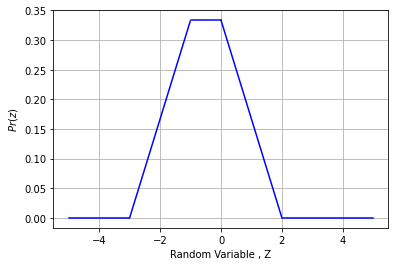
\includegraphics[width=.9\columnwidth] {solutions/ec/34/Figures/Assignment_3_PDF.png}
    \caption{The PDF of Z}
    \label{fig:The PDF of Z}
\end{figure}

\begin{figure}[!ht]
       \centering
    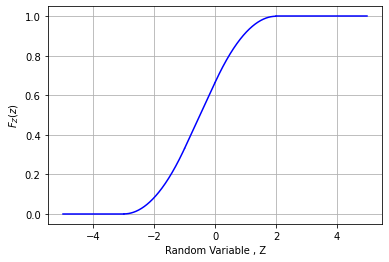
\includegraphics[width=.9\columnwidth] {solutions/ec/34/Figures/Assignment_3_CDF.png}
    \caption{The CDF of Z}
    \label{fig:The CDF of Z}
\end{figure}


\item Let X be the Gaussian random variable obtained by sampling the process at $t=t_i$ and let 
\begin{equation*}
Q(\alpha)={\int_{\alpha}^{\infty}}\dfrac{1}{\sqrt{2\pi}}e^{\frac{-y^2}{2}}dy
\end{equation*}
%
The probability that $[\textit{X}\leqslant1]$ is \dots
%

%\begin{enumerate}
%\begin{multicols}{2}
%\setlength\itemsep{1em}
%\item $
%1-Q(0.5)
%$
%\item $Q(0.5)$
%\item $Q\brak{\frac{1}{2\sqrt{2}}}
%$
%\item $
%1-Q\brak{\frac{1}{2\sqrt{2}}}
%$
%\end{multicols}
%\end{enumerate} 
%


\item Let Y and Z be the random variables obtained by sampling $X(t)$ at $t=2$ and $t=4$ respectively. Let W = Y-Z. The variance of W is
\begin{enumerate}
\begin{multicols}{4}
\setlength\itemsep{2em}
\item 13.36
\item 9.36
\item 2.64
\item 8.00

\end{multicols}
\end{enumerate}

%\item Let $(X_1,X_2)$ be independent random variables. $X_1$ has mean 0 and variance 1, while $X_2$ has mean 1 and variance 4. The mutual information I $(X_1;X_2)$ between $X_1$ and $X_2$ in bits is.......

\item Let the random variable X represent the number of times a fair coin needs to be tossed till two consecutive heads appear for the first time. The expectation of X is......

\item Let $X\in[0,1]$ and $Y\in[0,1]$ be two independent binary random variables. If $P(X=0) = p$ and $P(Y=0) = q$, then $P(X+Y\geqslant1)$ is equal to

\begin{enumerate}
\begin{multicols}{2}
\setlength\itemsep{1em}
{\small
\item $
pq + (1-p)(1-q)
$
\item pq
\item $p(1-q)$
\item $1-pq$
}
\end{multicols}
\end{enumerate}

\item Suppose A and B are two independent events with probabilities $P(A)\neq 0$ and $P(B)\neq0$. Let $\widetilde A$ and $\widetilde B$ be their complements. Which one of the following statements is FALSE?

\begin{enumerate}
\begin{multicols}{2}
\setlength\itemsep{1em}
{\scriptsize
\item $
P(A \cap B) = P(A)P(B)
$
\item $
P(A|B) = P(A)
$
\item $
P(A \cup B) = P(A)+P(B)
$
\item $
P(\widetilde A \cap \widetilde B) = P(\widetilde A)P(\widetilde B)
$
}
\end{multicols}
\end{enumerate}
\solution
\begin{enumerate}
    \item As $A,B$ are independent events, By definition,  
    \begin{align*}
        \Pr(A +B) &= \Pr(A)\Pr(B)
    \end{align*}
    Thus option 1 is true.
    \item 
    \begin{align*}
        \Pr(A|B) &= \frac{\Pr(A +B)}{\Pr(B)} \\
        &= \frac{\Pr(A)\Pr(B)}{\Pr(B)}\\
        &= \Pr(A)
    \end{align*}
    Thus option 2 is true.
    \item \begin{align*}
        \Pr(A B) &= \Pr(A) + \Pr(B) - \Pr(A +B) \\
        &= \Pr(A) + \Pr(B) - \Pr(A)\Pr(B)
    \end{align*}
    Thus option 3 is false. 
    \item \begin{align*}
        \Pr( A ^{\prime} + B ^{\prime}) &= \Pr(( A B )^{\prime} )\\
        &= 1- \Pr( A B)\\
        &= 1- \Pr(A) - \Pr(B) + \Pr(A +B) \\
        &= ( 1- \Pr(A) ) ( 1- \Pr(B) ) \\
        &= \Pr( A ^{\prime})\Pr( B ^{\prime})
    \end{align*}
    Thus option 4 is true.
\end{enumerate}
Hence, FALSE statement is option 3.
\item A digital communication system uses a repetition code for channel encoding/decoding. During transmission, each bit is repeated three times(0 is transmitted as 000, and 1 is transmitted as 111). It is assumed that the source puts out symbols independently and with equal probability. The decoder operates as follows: In a block of three received bits, if the number of zeros exceeds the number of ones, the decoder decides in favour of a 0, and if the number of ones exceeds the number of zeros, the decoder decides in favour of a 1. Assuming a binary symmetric channel with crossover probability p = 0.1, the average probability of error is ........
%
\\
\solution
Let Y be the bit sent by the sender and X be the number of 1's received by the receiver and p = 0.1 is the crossover probability
\\
{Case 1: Y = 0}
\begin{align}
    \Pr(X = i) &= \binom{n}{i}\times p^i\times (1-p)^{n-i}
\end{align}
When $X \geq 2 $ the receiver interprets it as 1, which is an error. And by Total Probability theorem we have\\
\begin{align}
P_1 = \frac{P(X = 2) + P(X = 3)}{\sum_{i=0}^3P(X = i)}
\end{align}
where $P_1$ is the probability of error when Y = 0
\\
{Case 2: Y = 1}
\begin{align}
\Pr(X = i) &= \binom{n}{i}\times p^{n-i}\times (1-p)^i
\end{align}
When $X \leq 1 $ the receiver interprets it as 0, which is an error. And by Total Probability theorem we have
\begin{align}
P_2 = \frac{\Pr(X = 0) + \Pr(X = 1)}{\sum_{i=0}^3\Pr(X = i)}
\end{align}
where $P_2$ is the probability of error when Y = 1
\begin{multline}
\sum_{i=0}^3\Pr(X = i) = 1\times 0.9^3 + 3\times 0.1\times 0.9^2 \\
+ 3\times 0.1^2 \times 0.9 + 1\times 0.1^3 = 1
\end{multline}
\begin{align}
P_1 &= 0.028\\
P_2 &= 0.028
\end{align}
The average probability is 
\begin{multline}
P_{avg} = \Pr(Y = 0)\times P_1 +\Pr(Y = 1)\times P_2\\ = 0.028 \end{multline}
\begin{table}[!ht]
\centering
\resizebox{\columnwidth}{!}{
\begin{tabular}{|c|c|c|c|c|c|}
\hline
     &X&0&1&2&3  \\
     \hline
     Y=0&$\Pr(X)$&0.729&0.243&0.027&0.001\\
     \hline
     Y=1&$\Pr(X)$&0.001&0.027&0.243&0.729\\
     \hline
\end{tabular}}
\caption{Probability of number of 1's recieved  }
\label{ec40:table:1}
\end{table}

\item Two random variables X and Y are distributed according to\\
{\centering $
f_{x,y}(x,y) = 
\begin{cases}
 (x+y) & 0 \leqslant x \leqslant 1   0 \leqslant y \leqslant 1 \\
 0 & \text{otherwise}.
 \end{cases}
 $ \\}
The probability $P(X+Y \leqslant 1)$ is .......

%\item A binary communication system makes use of the symbols "zero" and "one". There are channel errors. Consider the following events:
%\begin{itemize}
%\item $x_0$:a "zero" is transmitted
%\item $x_1$:a "one" is transmitted
%\item $y_0$:a "zero" is received
%\item $y_1$:a "one" is received
%\end{itemize}
%%
%The following probabilities are given: $P(x_0) = \frac{1}{2}$, $P(y_0|x_0)= \frac{3}{4}$, and $P(y_0|x_1)= \frac{1}{2}$. The information in bits that you obtain when you learn which symbol has been received (while you know that a "zero" has been transmitted) is .........

\item Let X be a zero mean unit variance Gaussian random variable. $E[|X|]$ is equal to .........

\item If calls arrive at a telephone exchange such that the time of arrival of any call is independent of the time of arrival of earlier or future calls, the probability distribution function of the toatl number of calls in a fixed time interval will be

\begin{enumerate}
\begin{multicols}{2}
\setlength\itemsep{2em}

\item Poisson
\item Gaussian
\item Exponential
\item Gamma

\end{multicols}
\end{enumerate}
\solution



\begin{table}[h!]
\centering
    \begin{tabular}{|p{0.14\linewidth}|p{0.35\linewidth}|p{0.16\linewidth}|p{0.16\linewidth}|}
    \hline
    \textbf{Symbol} & \textbf{Description} & \textbf{Property} & \textbf{Random}\\[0.5ex]
    \hline
    $T$ & Total time period & $T=n\Delta t$ &No\\
    \hline
    $n$ & Total Number of intervals &  &No\\
    \hline
    $\Delta t$ & One time interval & $\Delta t$=T/n & No\\
    \hline
    $k$ & Number of calls arrived during the time interval (0,$T$) & & Yes\\
    \hline
    $t_i$ & Denotes the time of arrival of each call in interval $(0,T)$ & &Yes\\
    \hline
    $p$ & Probability of receiving a call at time $t_i$ & &No\\
    \hline
    $\lambda$ & Average number of calls $(0,T)$ & $\lambda=np$ &No\\
    \hline
    $e$ & Euler's number & &No\\
    \hline
    \end{tabular}
\end{table}
Lets denote the fixed time interval by [0,$T$].
To find the probability of $k$ number of calls during this time interval, lets divide the interval into $n$ parts of equal length $\Delta t$.
Let us denote the probability of receiving a call at a particular time $t_i$ by $p$. Suppose the telephone exchange receives an average of $\lambda$ calls in time interval of length $T$.\\
Hence, we have
\begin{align}
    np=\lambda\\
    \implies p=\frac{\lambda}{n}
\end{align}
\begin{figure}[ht]
    \centering
    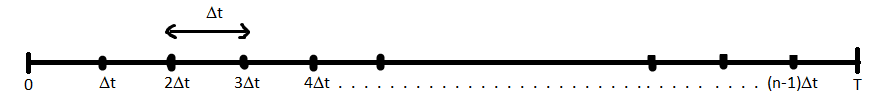
\includegraphics[width=\columnwidth]{solutions/ec/43/Figures/figure1.png}
    \caption{Figure showing division of time intervals}
    \label{ec43:figure_1}
\end{figure}
In Fig. \ref{ec43:figure_1}, the interval (0,$T$) has been divided into n equal parts, where length of each interval is $\Delta t$ and the number of calls in each interval is a random variable.
\begin{figure}[ht]
    \centering
    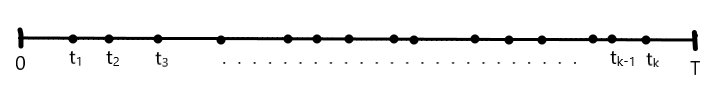
\includegraphics[width=\columnwidth]{solutions/ec/43/Figures/figure2.png}
    \caption{Figure showing times of arrival of $k$ calls}
    \label{ec43:Figure_2}
\end{figure}
$t_i$ where $i=\{1,2,3\cdots k\}$ are the time of arrival of $k$ calls in the interval $(0,T)$.\\

A call has probability $p$ for arriving at $t_i, \forall  i=\{1,2,\cdots k\}$ and the probability of 1-$p$ for not arriving at that instant.\\

In Binomial distribution we have certain number of intervals, i.e. $n$, with probability of arrival of each call as $p$ and for a binomial random variable $X=\{0,1\cdots n\}$, the probability of call arriving in any $k$ intervals is 
\begin{align}
    \pr{X=k}=\comb{n}{k}\cdot p^k\cdot(1-p)^k
\end{align} But in Poisson distribution, we essentially have infinite intervals, so $n\rightarrow\infty$. Thus, the probability expression changes to:
\begin{align}
   \lim_{n \to \infty}\pr{X=k}=\lim_{n \to \infty}\frac{n!}{k!(n-k)!}\left(\frac{\lambda}{n}\right)^k\left(1-\frac{\lambda}{n}\right)^{n-k}
\end{align}
\begin{multline}  \label{ec43:5}
    \lim_{n \to \infty}\pr{X=k}=\\
    \left(\frac{\lambda^k}{k!}\right)\lim_{n \to \infty}\frac{n!}{(n-k)!}\left(\frac{1}{n}\right)^k\left(1-\frac{\lambda}{n}\right)^n\left(1-\frac{\lambda}{n}\right)^{-k}
\end{multline}
Now lets take the limit of right-hand side one term at a time. We’ll do this in three steps. The first step is to find the limit of 
\begin{equation}
\begin{split}\label{ec43:6}
     \lim_{n \to \infty}\frac{n!}{(n-k)!n^k}
     &= \lim_{n \to \infty}\frac{n(n-1)(n-2)..(n-k+1)}{n^k}\\
    & = \lim_{n \to\infty}\left(\frac{n}{n}\right)\left(\frac{n-1}{n}\right)....\left(\frac{n-k+1}{n}\right)\\
   &= \lim_{n \to \infty}\left(1-\frac{1}{n}\right)\left(1-\frac{2}{n}\right)...\left(1-\frac{k-1}{n}\right)\\
    &=1\cdot1\cdot1........1\\
    &=1   
    \end{split}
\end{equation}
Now we have to find the limit of 
\begin{align}\label{ec43:7}
    \lim_{n \to \infty}\left(1-\frac{\lambda}{n}\right)^n 
\end{align}
We know that the definition $e$ is given as 
\begin{align}
    e=\lim_{x \to \infty}\left(1+\frac{1}{x}\right)^x
\end{align}
So, lets replace the value of $-\frac{n}{\lambda}$ by x in \eqref{ec43:7}, we get
\begin{align}\label{ec43:9}
    \lim_{n \to \infty}\left(1-\frac{\lambda}{n}\right)^n =\lim_{x \to \infty}\left(1+\frac{1}{x}\right)^{x(-\lambda)}=e^{-\lambda}
\end{align}
And the third part is to find the limit of 
\begin{align}
    \lim_{n \to \infty}\left(1-\frac{\lambda}{n}\right)^{-k}
\end{align}
As n approaches infinity, this term becomes $1^{-k}$ which is equal to one.
So,
\begin{align}\label{ec43:11}
    \lim_{n \to \infty}\left(1-\frac{\lambda}{n}\right)^{-k}=1
\end{align}
Now on substituting \eqref{ec43:6}, \eqref{ec43:9} and \eqref{ec43:11} in equation \eqref{ec43:5}, we get
\begin{multline}  
    \left(\frac{\lambda^k}{k!}\right)\lim_{n \to \infty}\frac{n!}{(n-k)!}\left(\frac{1}{n}\right)^k\left(1-\frac{\lambda}{n}\right)^n\left(1-\frac{\lambda}{n}\right)^{-k}=\\
    \left(\frac{\lambda^k}{k!}\right)(1)\left(e^{-\lambda}\right)(1)
\end{multline}
This just simplifies into
\begin{align}\label{ec43:final_equation}
    \pr{X=k}=\left(\frac{\lambda^k e^{-\lambda}}{k!}\right)
\end{align}
   \eqref{ec43:final_equation} is equal to probability density function of Poisson distribution, which gives us probability of $k$ successes per period, with given parameter of $\lambda$.\\
   
   $\therefore $The probability distribution function of the total
number of calls in a fixed time interval will be \textbf{Poisson} distribution.\\
Answer: Option(A)


\item Consider a communication scheme where the binary valued signal X satisfies $P\{X = +1\} = 0.75$ and $P\{X = -1\} = 0.25$. The received signal $Y = X+Z$, where Z is a Gaussian random variable with zero mean and variance $\sigma^2$. The received signal Y is fed to the threshold detector. The output of the threshold detector $\hat X$ is:\\
{\centering $
{\hat X}= 
\begin{cases} 
+1 & Y> \tau \\
-1 & Y \leqslant \tau 
\end{cases}
$\\}
To achieve minimum probability of error $P\{\hat X \neq X\}$, the threshols $ \tau$ should be

\begin{enumerate}
\begin{multicols}{2}
\setlength\itemsep{2em}

\item strictly positive
\item zero
\item strictly negative
\item strictly positive, zero or strictly negative depending on the nonzero value of $\sigma ^2$

\end{multicols}
\end{enumerate}

\item Consider a discrete-time channel $Y = X+Z$, where the additive noise Z is signal-dependent. In particular, given the transmitted symbol $X \in \{-a,+a\}$ at any instant, the noise sample Z is chosen independently from a Gaussian distribution with mean $\beta X$ and unit variance. Assume a threshold detector with zero threshold at the receiver.\\
When $\beta = 0$, the BER was found to be $Q(a) = 1 \times {10^-8}$.\\
$$
\bigg(Q(v)= \dfrac{1}{\sqrt{2 \pi}} \int_{v}^{\infty} e^{\frac{-u^2}{2}}du$$, and for $v>1$, use $Q(v) \approx e^{\frac{-v^2}{2}} \bigg)$ \\
When $\beta = -0.3$, the BER is closet to

\begin{enumerate}
\begin{multicols}{2}
\setlength\itemsep{2em}

\item $10^-7$
\item $10^-6$
\item $10^-4$ \label{option C}
\item $10^-2$

\end{multicols}
\end{enumerate}
%
\solution

Given that the threshold of the detector is zero. Define a detector function $g$ such that
\begin{align}
g(Y) = 
\begin{cases}
+a & Y>0 \\
-a & Y<0
\end{cases}
\end{align}
It is given that $X \in \{ -a, a\}$ is a random variable.
\begin{align}
\therefore \Pr(X=a) = \Pr(X=-a) = \dfrac{1}{2}
\end{align}
Since the noise in the signal, $Z$ is chosen independently from a Gaussian distribution with mean $ \mu = \beta X$ and unit variance, it follows that
\begin{align}
F_Z(z) &= \int_{-\infty}^{z} \dfrac{1}{\sqrt{2\pi}} \exp \left( \dfrac{-(z - \beta X)^2}{2} \right) dz \\
&= \int_{-\infty}^{z - \beta X} \dfrac{1}{\sqrt{2\pi}} \exp \left( \dfrac{-z^2}{2} \right) dz \\
&= \int_{\beta X-z}^{\infty} \dfrac{1}{\sqrt{2\pi}} \exp \left( \dfrac{-z^2}{2} \right) dz \\
&= Q(\beta X - z) \label{eqn 2.0.7}
\end{align}
Also, it is easy to see that 
\begin{align}
Q(-v) = 1 - Q(v) \; \forall \; v \in \mathbb{R} \label{eqn 2.0.8}
\end{align}
The detector can record erroneous bits in the signal iff
\begin{align}
X>0 \; &, \; g(Y) = -a \; (\text{Call this BER}_{+a}) \text{ or}\\
X<0 \; &, \; g(Y) = a \; (\text{Call this BER}_{-a})
\end{align}
\begin{align}
\therefore \text{BER}_{+a} % &= \Pr(g(Y) = -a \;,\; X = a)\\
&= \Pr(g(Y) = -a \;|\; X = a) \Pr(X=a)\\
&= \Pr(Y < 0 \;|\; X = a) \Pr(X=a)\\
&= \dfrac{1}{2} \times \Pr(X+Z < 0 \;|\; X = a) \\
% &= \dfrac{1}{2} \times \Pr(a+Z < 0 \;|\; X = a) \\
% &= \dfrac{1}{2} \times \Pr(Z < -a \;|\; X = a) \\
&= \dfrac{1}{2} \times F_Z(-a)\\
&= \dfrac{1}{2} \times Q(\beta X + a) \; \text{ (From (\ref{eqn 2.0.7}))}\\
% &= \dfrac{1}{2} \times Q(a \beta + a)\\
&= \dfrac{1}{2} \times Q(a(1+\beta))
\end{align}
\begin{align}
\text{BER}_{-a} % &= \Pr(g(Y) = a \;,\; X = -a)\\
&= \Pr(g(Y) = a \;|\; X = -a) \Pr(X=-a)\\
&= \Pr(Y > 0 \;|\; X = -a) \Pr(X=-a)\\
&= \dfrac{1}{2} \times \Pr(X+Z > 0 \;|\; X = -a) \\
% &= \dfrac{1}{2} \times \Pr(Z-a > 0 \;|\; X = -a) \\
% &= \dfrac{1}{2} \times \Pr(Z > a \;|\; X = -a) \\
&= \dfrac{1}{2} \times \left( 1 - F_Z(a) \right) \\
&= \dfrac{1}{2} \times \left( 1 - Q(\beta X -a) \right) \; \text{ (From (\ref{eqn 2.0.7}))}\\
% &= \dfrac{1}{2} \times \left( 1 - Q(-a \beta -a) \right) \\
&= \dfrac{1}{2} \times Q(a(1+\beta)) \; \text{ (From (\ref{eqn 2.0.8}))}
\end{align}
\begin{align}
\therefore \text{BER} &= \text{BER}_{+a} + \text{BER}_{-a}\\
&= Q(a(1+\beta))
\end{align} 
\begin{figure}[!hbt]
    \centering
	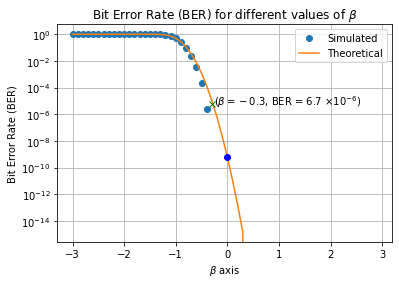
\includegraphics[width=\columnwidth]{solutions/ec/45/Figures/Figure_3.png}
    \caption{Theory vs Simulated plot of BER}
    \label{CDF_Y}
\end{figure}
When $\beta = 0$, it is given that 
\begin{align}
\text{BER} = Q(a) &= 10^{-8}
\end{align}
On computing, $Q(1) \approx 0.16$. Since $Q(a)<Q(1)$, it is easy to see that $a>1$ (as $Q(x)$ is a decreasing function)
\begin{align}
\therefore e^{-a^2 / 2} &= 10^{-8}\\
\Leftrightarrow a &\approx 6.069
\end{align}
When $\beta = -0.3$,
\begin{align}
\text{BER} = Q(a(1+\beta)) &= Q(6.069 \times (1-0.3))\\
&= Q(6.069 \times 0.7)\\
&= Q(4.249)\\
&\approx \exp (-\dfrac{4.249^2}{2})\\
&\approx 1.2 \times 10^{-4}
\end{align}
Therefore, when $\beta = -0.3$, BER is closest to $10^{-4}$ and option \ref{option C} is correct.


\item Consider the random process\\
$ X(t) = U+Vt$,\\
where U is a zero-mean Gaussian random variable and V is a random variable distributed between 0 and 2. Assume that U and V are statistically independent. The mean value of the random  process at t=2 is........
%
\solution
Here U is a gaussian random variable of mean 0 and Let us consider V is uniformly distributed random variable in $(0,2)$.
\begin{table}[h]
\centering
\begin{tabular}{|c|c|c|c|}
\hline
   Random Variable             & U & V & X(t)  \\ \hline
Expected Value & 0 & 1 & t\\ \hline
\end{tabular}
\caption{Random Variables and Expected Values}
\label{tab:expected values}
\end{table}

From Table \ref{tab:expected values} we can deduce that,
\begin{align}
    E\sbrak{X(t)}&=E\sbrak{U+Vt}\\
    E\sbrak{X(t)}&=E\sbrak{U}+tE\sbrak{V}\\
    E\sbrak{X(t)}&=0+t\\
    E\sbrak{X(t)}&=t\\
    E\sbrak{X(2)}&=2
\end{align}
 $ \therefore$ mean of random process X(t) at 2 is 2.


\item Consider the Z-channel given in Fig. \ref{fig:1}. The input is 0 or 1 with equal probability.
\begin{figure}[!h]
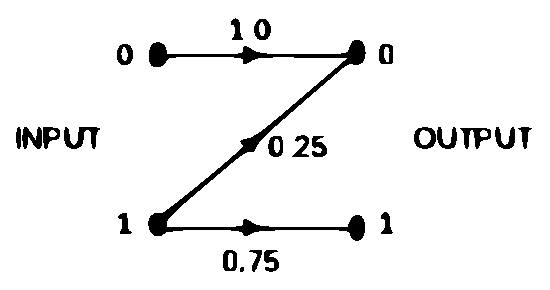
\includegraphics[width=\columnwidth]{./figs/figure1.eps}
\caption{}
\label{fig:1}
\end{figure}



If the output is 0, the probability that the input is also 0 equals......

\item If P and Q are two random events, then the following is TRUE:

\begin{enumerate}

\item Independence of P and Q implies that $\Pr{P \cap Q} = 0$
\item $\Pr(P \cup Q)\geqslant \Pr(P)+\Pr(Q)$
\item If P and Q are mutually exclusive, then they must be independent
\item $\Pr(P \cap Q)\leqslant \Pr(P)$

\end{enumerate}
%
\solution
\begin{enumerate}
	    \item  Independence of P and Q means if P happens, then outcome of Q won't be affected by that.
	    	so \begin{align}
		\pr{P/Q} &= \pr{P} \\
		\frac{\pr{P Q}}{\pr{Q}} &= \pr{P} \\
		\implies  \pr{P Q} &= \pr{P}.\pr{Q}
	\end{align}
	This is what we can say hence (A) is wrong 
	\item As \begin{align}
		\pr{P + Q} &= \pr{P} + \pr{Q} -\pr{P Q} \\
		\pr{P + Q} + \pr{P Q} &= \pr{P} + \pr{Q} \\
		\pr{P Q} &\geq 0 \\
		\implies \pr{P} + \pr{Q} &\geq \pr{P + Q}
	\end{align}
	Hence (B) is also wrong 
    \item When P and Q are mutually exclusive, then either P occurs or Q occurs but not both simultaneously.So if P happens, chance of Q happening gets ruled out and vice-versa.\\Mutually exclusive refers
    \begin{align}
        \pr{P Q} &= 0 \\
        \pr{P Q} &\neq \pr{P}.\pr{Q}
    \end{align}Hence, mutually exclusive events may not be independent.\\Hence (C) is also wrong
	\item As \begin{align}
		\pr{Q/P} &= \frac{\pr{P Q}}{\pr{P}} 
	\end{align}
	And \begin{align}
		\pr{Q/P} &\leq 1\\
		\frac{\pr{P Q}}{\pr{P}} &\leq 1\\ 
		\pr{P Q} &\leq \pr{P}
	\end{align}
	Hence (D) is correct.
	
	\end{enumerate}
	
\item A fair coin is tossed three times in succession. If the first toss produces a head, then the probability of getting exactly two heads in three tosses is:

\begin{enumerate}
\begin{multicols}{2}
\setlength\itemsep{1em}

\item $\frac{1}{8}$
\item $\frac{1}{2}$
\item $\frac{3}{8}$
\item $\frac{3}{4}$

\end{multicols}
\end{enumerate}

\item The probability density function (PDF) of a random variable X is as shown in Fig. \ref{fig:2}.
\begin{figure}[!h]
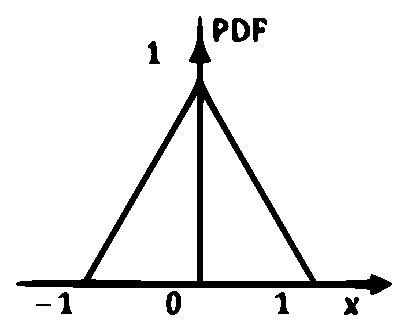
\includegraphics[width=\columnwidth]{./figs/figure2.eps}
\caption{}
\label{fig:2}
\end{figure}

The corresponding cumulative distribution function (CDF) has the form\\

\begin{enumerate}
\begin{multicols}{2}
\setlength\itemsep{4em}

\item Fig. \ref{fig:3}

%\includegraphics{figure3.eps}
\item Fig. \ref{fig:4}

%\includegraphics{figure4.eps}
\item Fig. \ref{fig:5}

% \includegraphics{figure5.eps}
\item Fig. \ref{fig:6}


%\includegraphics{figure6.eps}

\end{multicols}
\end{enumerate}
\begin{figure}[!h]
\includegraphics[width=\columnwidth]{./figs/figure3.eps}
\caption{}
\label{fig:3}
\end{figure}
\begin{figure}[!h]
\includegraphics[width=\columnwidth]{./figs/figure4.eps}
\caption{}
\label{fig:4}
\end{figure}
\begin{figure}[!h]
\includegraphics[width=\columnwidth]{./figs/figure5.eps}
\caption{}
\label{fig:5}
\end{figure}

\begin{figure}[!h]
\includegraphics[width=\columnwidth]{./figs/figure6.eps}
\caption{}
\label{fig:6}
\end{figure}



%\item Consider a binary, digital communication system which uses pulses g(t) and -g(t) for transmitting bits over an AWGN channel. If the receiver uses a matched filter, which one of the following pulses will give the minimum probability of bit error?\\
%
%\begin{enumerate}
%\begin{multicols}{2}
%\setlength\itemsep{4em}
%
%
%\item Fig. \ref{fig:8}
%\item Fig. \ref{fig:9}
%\item Fig. \ref{fig:10}
%\item Fig. \ref{fig:11}
%
%\end{multicols}
%\end{enumerate}
%\begin{figure}[!h]
%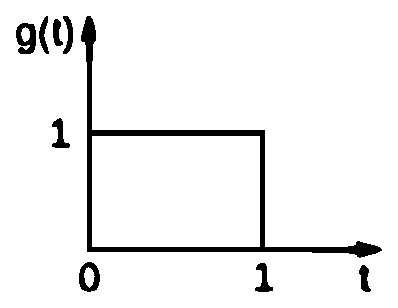
\includegraphics[width=\columnwidth]{./figs/figure8.eps}
%\caption{}
%\label{fig:8}
%\end{figure}
%\begin{figure}[!h]
%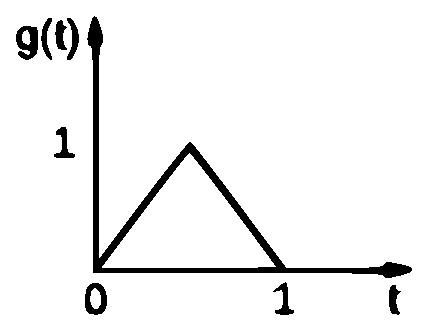
\includegraphics[width=\columnwidth]{./figs/figure9.eps}
%\caption{}
%\label{fig:9}
%\end{figure}
%\begin{figure}[!h]
%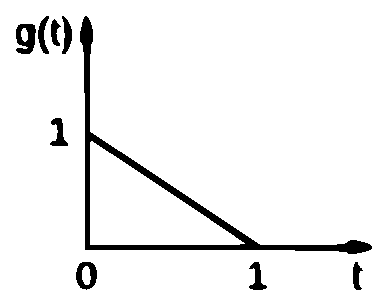
\includegraphics[width=\columnwidth]{./figs/figure10.eps}
%\caption{}
%\label{fig:10}
%\end{figure}
%\begin{figure}[!h]
%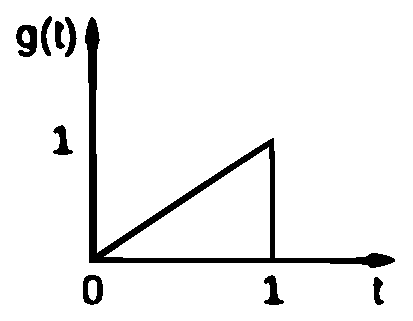
\includegraphics[width=\columnwidth]{./figs/figure11.eps}
%\caption{}
%\label{fig:11}
%\end{figure}


\item The distribution function $f_x(x)$ of a random variable X is shown in Fig. \ref{fig:12}. The probability that X=1 is
%
\begin{figure}[!h]
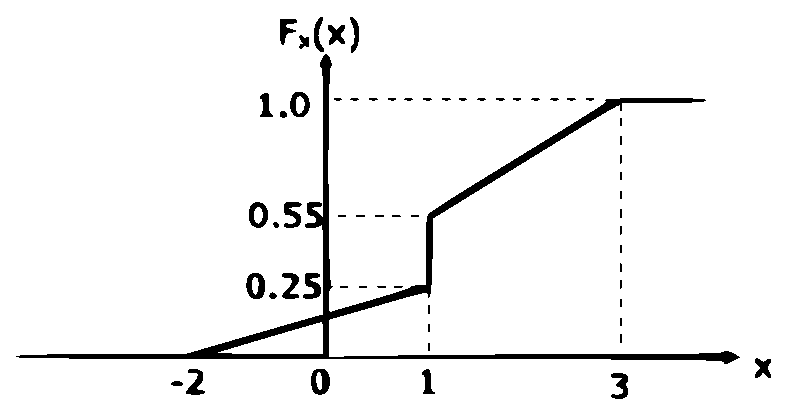
\includegraphics[width=\columnwidth]{./figs/figure12.eps}
\caption{}
\label{fig:12}
\end{figure}


\begin{enumerate}
\begin{multicols}{2}
\setlength\itemsep{1em}

\item Zero
\item 0.25
\item 0.55
\item 0.30

\end{multicols}
\end{enumerate}


%\begin{center}
%\centering\underline{\textbf{Common Data for the following two Questions :}}
%\end{center}

%\item Let $X$ be a random variable with probability density function $f \in \{f_0,f_1\},$ where 
%
%$ 
%f_0(x)=
%\begin{cases}
%2x & 0<x<1 \\
%0 & \text{otherwise}
%\end{cases}
%$ \\
%
%$ 
%f_1(x)=
%\begin{cases}
%3x^2 &  0<x<1 \\
%0 & \text{otherwise}
%\end{cases}
%$\\
%
%For testing the null hypothesis $H_0:f \equiv f_0$ against the alternative hypothesis $H_1:f \equiv f_1$ at level of significance $\alpha = 0.19$, the power of the most powerful test is
%
%\begin{enumerate}
%\begin{multicols}{2}
%\setlength\itemsep{2em}
%
%\item $ 0.729$
%\item $ 0.271$
%\item $ 0.615$
%\item $ 0.385$
%
%\end{multicols}
%\end{enumerate}
%

%\item The variance of the random variable $X$ is
%
%\begin{enumerate}
%\begin{multicols}{2}
%\setlength\itemsep{2em}
%
%\item $ \frac{1}{12}$
%\item $ \frac{1}{4}$
%\item $ \frac{7}{12}$
%\item $ \frac{5}{12}$
%
%\end{multicols}
%\end{enumerate}
%
%
%\item The covariance between the random variables $X$ and $Y$ is
%
%\begin{enumerate}
%\begin{multicols}{2}
%\setlength\itemsep{2em}
%
%\item $ \frac{1}{3}$\\
%\item $ \frac{1}{4}$\\
%\item $ \frac{1}{6}$\\
%\item $ \frac{1}{12}$\\
%
%\end{multicols}
%\end{enumerate}

\item Let the probability density function of a random variable $X$ be 
\begin{center}
$ 
f(x)=
\begin{cases}
x & 0\leq\ x< \frac{1}{2}\\
c(2x-1)^2 &  \frac{1}{2}<x\leq\ 1\\
0 & \text{otherwise}.
\end{cases}
$\\ 
\end{center}


Then,the value of $c$ is equal to \underline{\hspace{3cm}}
\\
\solution
For a probability density function of a continuous random variable, 
\begin{equation}
    \int \limits_{-\infty}^{\infty} f_X(x) \, dx = 1 \label{ec52:eq1}
\end{equation}
\begin{align}
    \int \limits_{-\infty}^{\infty} f_X(x) \, dx &=  \int \limits_0^{1/2} f_X(x) \, dx + \int \limits_{1/2}^1 f_X(x) \, dx\\
    &= \left. \frac{1}{2} (x)(x) \right\rvert_{x = \frac{1}{2}} + \int \limits_{1/2}^1 c(2x-1)^2 \, dx\\
    &= \frac{1}{2}\times\frac{1}{2}\times\frac{1}{2} + c\rsbrak{\brak{\frac{4x^3}{3} - 2x^2 + x}}_{1/2}^1 \\
    &= \frac{1}{8} + c\brak{\frac{1}{3} - \frac{1}{6}} \\
    &= \frac{1}{8} + \frac{c}{6}  \label{ec52:eq6}\\
    \intertext{from \eqref{ec52:eq1}  and \eqref{ec52:eq6} we get }
    1 &= \frac{1}{8} + \frac{c}{6} \\
    \therefore c &= \frac{21}{4}
\end{align}
\begin{figure}[!ht]
\centering
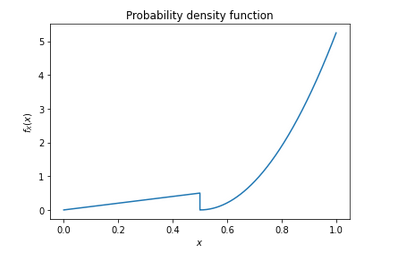
\includegraphics[width=\columnwidth]{solutions/ec/52/figures/pdfimage.png}
\caption{Graph of $f_X(x)$}
\end{figure}
\begin{equation} \label{ec52:eq9}
    F_X(x) = f_X(X<=x) = \int\limits_{-\infty}^x f_X(x) \, dx
\end{equation}
from $f_X(x)$ and equation \eqref{ec52:eq9}, 
\begin{displaymath}
    F_X(x)=\lcbrak{
                    \begin{array}{ll}
                        0 & x\leq 0 \\\\
		                \frac{x^2}{2} &   0 \leq x \leq \frac{1}{2}  \\\\
		                \frac{1}{8} + \frac{7}{8} (2x-1)^3 & \frac{1}{2} \leq x \leq 1 \\\\
		                1 & x>1\\
	                \end{array}    
                }
\end{displaymath}
\begin{figure}[!ht]
\centering
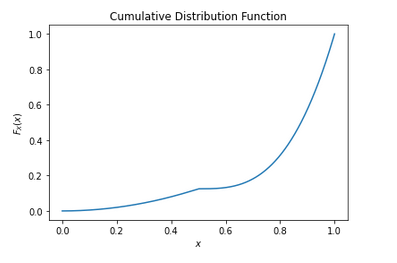
\includegraphics[width=\columnwidth]{solutions/ec/52/figures/cdfimage.png}
\caption{Graph of $F_X(x)$}
\end{figure}


\item Suppose $X$ and $Y$ are two random variables such that $aX + bY$ is a normal random variable for all $a,b \in \mathbb{R}$. Consider the following statements P,Q,R and S:


 (P): $X$ is a standard normal random variable.\\
 (Q): The conditional distribution of $X$ given $Y$ is normal.\\
 (R): The conditional distribution of $X$ given $X$ + $Y$ is normal.\\
 (S): $X$ - $Y$ has mean $0$.\\

Which of the above statements ALWAYS hold TRUE?
\begin{enumerate}
\begin{multicols}{2}
\setlength\itemsep{2em}

\item both P and Q
\item both Q and R
\item both Q and S
\item both P and S

\end{multicols}
\end{enumerate}

 
\item Let $X$ be a random variable with the following cumulative distribution function: 

\begin{center}
$ 
F(x)=
\begin{cases}
0 & x<0 \\
x^2 & 0\leq\ x <\frac{1}{2}\\
\frac{3}{4} & \frac{1}{2}\leq\ x<1\\
1 & x\geq\ 1.
\end{cases}
$\\ 

\end{center}
Then $P\brak{\frac{1}{4}<X<1}$ is equal to \underline{\hspace{3cm}}
\\
\solution
\begin{align}
 P ( a \textless x \textless b ) =  F(b) - F(a) \end{align}
We want, 
 \begin{align}
S&= P ( {\dfrac{1}{4}}  \textless  X \textless  1)\\
S&= F(1) - F(\dfrac{1}{4})  \\
S&= \dfrac{3}{4} - \dfrac{1^2}{4^2} \\
S&= \dfrac{11}{16}
\end{align}
Hence, P( ${\frac{1}{4}}$ $ \textless $ X $\textless $ 1) is equal to $\frac{11}{16}$

\begin{figure}[!ht]
\centering
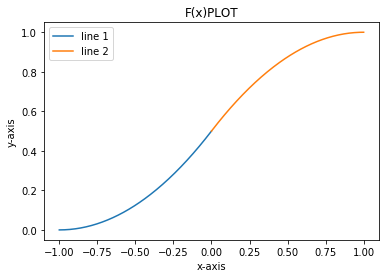
\includegraphics[width=0.5\textwidth]{solutions/ec/54/codes/graph.png}
\label{ec54:fig:graph.png}
\end{figure}



 


\item Let $X_1$ be an exponential random variable with mean 1 and $X_2$ a gamma random variable with mean 2 and variance 2. If $X_1$ and $X_2$ are independently distributed,then $P(X_1<X_2)$ is equal to \underline{\hspace{3cm}}
\\
\solution
\begin{enumerate}
    \item Given that $X_1$ is an exponential random variable. Let the P.D.F of $X_1$ be
    \begin{align}
    p_{X_1}(x_1)=
        \begin{cases}
        \lambda e^{-\lambda x_1} & x_1 \geq 0\\
        0 & x_1<0
        \end{cases}
    \end{align}
    C.D.F of $x_1$ is :
    \begin{align}
    \begin{split}
        F_{X_1}(x_1)&=\int_{-\infty}^{x_1} p_{X_1}(x_1) dx_1\\
        &=\int_{-\infty}^0 p_{X_1}(x_1) dx_1+\int_{0}^{x_1} p_{X_1}(x_1) dx_1\\
        &=\int_{-\infty}^0 0 \times dx_1+\int_{0}^ {x_1} \lambda e^{-\lambda x_1} dx_1\\
        &=1-e^{-\lambda x_1}\label{ec55:eq:0.0.2}
        \end{split}
    \end{align}
    \begin{align}
    \text{ As mean}=\lambda\\
     \text{ Given that mean}=1\\
     \text{so } \lambda=1 \label{ec55:eq:0.0.5}
    \end{align} 
     
    \item Given that $X_2$ is an gamma random variable.Let the P.D.F of $X_2$ be:
    \begin{align}
        p_{X_2}(x_2)=
        \begin{cases}
            \frac{a^b x_2^{b-1}e^{-ax_2}}{\Gamma(b)} & x_2\geq 0\\
            0 & x_2<0
        \end{cases}\label{ec55:eq:0.0.6}
    \end{align}
    \begin{align}
       \text{ Since mean}=\frac{b}{a}=2\label{ec55:eq:0.0.7}\\
         \text{Also,variance}=\frac{b}{a^2}=2\label{ec55:eq:0.0.8}
    \end{align}
  From \eqref{ec55:eq:0.0.7} and \eqref{ec55:eq:0.0.8}
  \begin{align}
      b=2,a=1\label{ec55:eq:0.0.9}
  \end{align}
  Since the total probability of $X_2$ is 1 \\
  so,\begin{align}
      \int_{-\infty}^\infty p_{X_2}(x_2) dx_2=1
      \end{align}
      \begin{align}
      \int_{-\infty} ^0 p_{X_2}(x_2)
     dx_2+\int_{0}^\infty p_{X_2}(x_2) dx_2&=1\\
      \int_{-\infty} ^0 0\times dx_2+\int_{0}^\infty \frac{a^b x_2^{b-1}e^{-ax_2}}{\Gamma(b)} dx_2&=1
      \end{align}
      \begin{align}
      \frac{a^b}{\Gamma(b)} \int_{0}^\infty x_2^{b-1}e^{-ax_2} dx_2&=1
      \end{align}
      \begin{align}
          \int_{0}^\infty x_2^{b-1}e^{-ax_2} dx_2&=\frac{\Gamma(b)}{a^b}\label{ec55:eq:0.0.14}
  \end{align}
  now substituting $a+\lambda$ for a in \eqref{ec55:eq:0.0.14} gives 
  \begin{align}
      \int_{0}^\infty x_2^{b-1}e^{-(a+\lambda)x_2} dx_2&=\frac{\Gamma(b)}{(a+\lambda)^b}\label{ec55:eq:0.0.15}
  \end{align}
  Now we have to find $P(X_1<X_2)$\\
  \item Given that $X_1$ and $X_2$ are independent random variables,so
  \begin{align}
     P(X_1<X_2|X_2)=F_{X_1}(X_2)=1-e^{-\lambda X_2}\label{ec55:eq:0.0.16}
  \end{align}
  Now,
\begin{align}
      P(X_1<X_2)&=\int_{0}^\infty F_{X_1}(X_2) \times p_{X_2}(x_2)dx_2
      \end{align}
      from \eqref{ec55:eq:0.0.6},\eqref{ec55:eq:0.0.16}
  \begin{align}
     P(X_1<X_2)=\int_{0}^\infty (1-e^{-\lambda X_2})\times \frac{a^b x_2^{b-1}e^{-ax_2}}{\Gamma(b)} dx_2
     \end{align}
     \begin{align}
     P(X_1<X_2)=\frac{a^b}{\Gamma(b)}\int_{0}^\infty x_2^{b-1}(e^{-ax_2}-e^{-(a+\lambda)x_2})dx_2
  \end{align}
      from \eqref{ec55:eq:0.0.14} and \eqref{ec55:eq:0.0.15}
      \begin{align}
     P(X_1<X_2)&=\frac{a^b}{\Gamma(b)}\brak{\frac{\Gamma(b)}{a^b}-\frac{\Gamma(b)}{(a+\lambda)^b}}
     \end{align}
 \begin{align}
      P(X_1<X_2)=1-\frac{a^b}{(a+\lambda)^b}
 \end{align}
 \begin{align}
     P(X_1<X_2)=1-\brak{\frac{a}{a+\lambda}}^b
 \end{align}
 from \eqref{ec55:eq:0.0.5} and \eqref{ec55:eq:0.0.9}
 \begin{align}
     P(X_1<X_2)&=1-\brak{\frac{1}{1+1}}^2\\
     P(X_1<X_2)&=1-\frac{1}{4}=\frac{3}{4}
 \end{align}
\end{enumerate}

\begin{center}
\centering\underline{\textbf{Common Data for the next two Questions :}}
\end{center}


Let $X$ and $Y$ be jointly distributed random variables such that the conditional distribution of $Y$, given $X$ =$x$, is uniform on the interval $(x-1,x+1)$. Suppose $E(X)=1$ and $Var(X)=\frac{5}{3}$.
\\
\item The mean of the random variable $Y$ is 
\\
\begin{enumerate}
\begin{multicols}{2}
\setlength\itemsep{2em}

\item $ \frac{1}{2}$\\
\item $1$\\
\item $ \frac{3}{2}$\\
\item $2$

\end{multicols}
\end{enumerate}
\solution
We know that,
\begin{equation}
    f_{Y|X=x}(y)=\frac{f(x,y)}{f_{X}(x)} \label{ec56:eq:2.0.1}
\end{equation}
Given that $f_{Y|X=x}(y)$ is uniform over the interval (x-1,x+1).
\begin{equation}
    \Rightarrow f_{Y|X=x}(y)=
    \begin{cases}
    \frac{1}{2} & y \in \brak{x-1,x+1}\\
    0 & \text{otherwise}
    \end{cases}\label{ec56:eq:2.0.2}
\end{equation}
Given $E(X)=1$
\begin{equation}
    \Rightarrow \int_{-\infty}^{\infty}x f_{X}(x)dx=1 \label{ec56:eq:2.0.3}
\end{equation}
Now consider $E(Y|X=x)$,
\begin{equation}
    E(Y|X=x)=\int_{-\infty}^{\infty}yf_{Y|X=x}(y)dy
\end{equation}
From \eqref{ec56:eq:2.0.2} it simplifies to,
\begin{multline}
    \Rightarrow E(Y|X=x)=\int_{-\infty}^{x-1}yf_{Y|X=x}(y)dy+\\ \int_{x-1}^{x+1}yf_{Y|X=x}(y)dy+\int_{x+1}^{\infty}yf_{Y|X=x}(y)dy
\end{multline}
\begin{align}
    \Rightarrow E(Y|X=x)&=\int_{x-1}^{x+1}y\brak{\frac{1}{2}}dy\\
    &=x
\end{align}
Now we can write ,\\
\begin{align}
    E(Y)&=\int_{-\infty}^{\infty}E(Y|X=x)f_{X}(x)dx\\
    &=\int_{-\infty}^{\infty}xf_{X}(x)dx\\
    &=E(X)
\end{align}
From \eqref{ec56:eq:2.0.3} we get 
\begin{equation}
    E(Y)=1.
\end{equation}
\item The variance of the random variable $Y$ is 
\\
\begin{enumerate}
\begin{multicols}{2}
\setlength\itemsep{2em}

\item $ \frac{1}{2}$\\
\item $ \frac{2}{3}$\\
\item $1$\\
\item $2$

\end{multicols}
\end{enumerate}
\solution
\begin{align}
    Var(Y|X=x)&=\int_{-\infty}^{\infty}(y-E(Y))^2f_{Y|X=x}(y)dy\\
    &=\int_{x-1}^{x+1}(y-1)^2\brak{\frac{1}{2}}dy
\end{align}
\begin{align}
    Var(Y)&=\int_{-\infty}^{\infty}Var(Y|X=x)f_{X}(x)dx\\
    &=\brak{\frac{1}{2}}\int_{x-1}^{x+1}\brak{y^2-2y+1}dy\\
    &=\brak{\frac{1}{2}}\brak{\frac{6x^2+2}{3}+2-4x}\\
    &=x^2-2x+\frac{4}{3}
\end{align}
\begin{align}
  Var(Y)=\int_{-\infty}^{\infty}\brak{x^2-2x+\frac{4}{3}}f_{X}(x)dx\\
   =\int_{-\infty}^{\infty}x^2f_{X}(x)dx-2\int_{-\infty}^{\infty}xf_{X}(x)dx+\\\label{ec57:eq:0.0.19}\frac{4}{3}\int_{-\infty}^{\infty}f_{X}(x)dx\
 \end{align}
\begin{align}
  f_{X}(x)dx=1\\\label{ec57:eq:0.0.20}
 Var(X)=\int_{-\infty}^{\infty}x^2f_{X}(x)dx=\frac{5}{3}\\\label{ec57:eq:0.0.21}
 E(x)=\int_{-\infty}^{\infty}xf_{X}(x)dx=1\\\label{ec57:eq:0.0.22}
 \end{align}
 From \eqref{ec57:eq:0.0.19},\eqref{ec57:eq:0.0.20},\eqref{ec57:eq:0.0.21}and \eqref{ec57:eq:0.0.22} we get
 \begin{align}
     Var(Y)&=\frac{5}{3}-2+\frac{4}{3}\\
     &=1
 \end{align}
\textbf{$\therefore$ Option C is true}


\item Let the random variable $X$ have the distribution function: 
\begin{center}
$ 
F(x)=
\begin{cases}
0 &  \ x<0 \\
\frac{x}{2} &  \ 0\leq\ x <1 \\
\frac{3}{5} &  \ 1\leq\ x<2\\
\frac{1}{2}+\frac{x}{8} &  \ 2\leq\ x<3\\
1 &  \ x\geq\ 3.
\end{cases}
$\\ 
\end{center}

Then $P\brak{2 \leq\ X<4}$ is equal to \underline{\hspace{3cm}}
 \\
\solution

Given F(X) is the CDF of the random variable $X$.
\\$P(2\le X<4)$ will be the sum of all the probabilities of values the random variable $X$ can take in $[2,4)$.
\\So it is the difference between CDF values of the random variable X at X=4- and at X=2-.
\\Therefore,
\begin{align}
P(2\le X<4)&=\lim_{X \to 4-}{F(X)}-\lim_{X \to 2-}{F(X)}
 \\     &= \lim_{X \to 4-}{1}-\lim_{X \to 2-}{\frac{3}{5}}
 \\ &= 1-\frac{3}{5}
 \\ &=\frac{2}{5}=0.4
\end{align}
Hence,$P(2\le X<4) = 0.4$.\begin{figure}[ht]
    \centering
    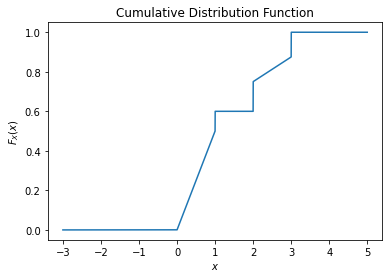
\includegraphics[width=\columnwidth]{solutions/ec/58/CDF.png}
    \caption{CDF of X}
    \label{fig:my_label}
\end{figure}



\item Let $X$ be a random variable having the distribution function: 
\begin{center}
$ 
F(x)=
\begin{cases}
0 &  \ x<0 \\
\frac{1}{4} &  \ 0\leq\ x <1 \\
\frac{1}{3} &  \ 1\leq\ x<2\\
\frac{1}{2} &  \ 2\leq\ x<\frac{11}{3}\\
1 &  \ x\geq\ \frac{11}{3}.
\end{cases}
$\\ 
\end{center}

Then $E(X)$ is equal to \underline{\hspace{3cm}}
\\
\item Let $X$ and $Y$ be two random variables having the joint probability density function

\begin{center}
$ 
f(x,y)=
\begin{cases}
2 &  \ 0<x<y<1 \\
0 & \text{otherwise}.
\end{cases}
$\\ 
\end{center}

Then the conditional probability $P \brak{X \leq\ \frac{2}{3} | Y=\frac{3}{4}}$ is equal to \underline{\hspace{3cm}}

\begin{enumerate}
\begin{multicols}{4}
\setlength\itemsep{2em}

\item $
\frac{5}{9}
$
\item $
\frac{2}{3}
$
\item $
\frac{7}{9}
$
\item $
\frac{8}{9}
$


\end{multicols}
\end{enumerate}

\item Let $\Omega= (0,1]$ be the sample space and let $P(\cdot)$ be a probability function defined by 

\begin{center}
$ 
P((0,x])=
\begin{cases}
\frac{x}{2} &  \ 0 \leq\ x< \frac{1}{2} \\
x &  \  \frac{1}{2} \leq\ x \leq\ 1.
\end{cases}
$\\ 
\end{center}

Then $P\brak{\lbrace\frac{1}{2}\rbrace}$ is equal to \underline{\hspace{3cm}}
\\

\item Suppose the random variable $U$ has uniform distribution on $[0,1]$ and $X= -2\log U$. The density of $X$ is

\begin{enumerate}

\item $ 
f(x)=
\begin{cases}
e^{-x} &  \ x>0\\
0 & \text{otherwise}.
\end{cases}
$\\ 

\item $ 
f(x)=
\begin{cases}
2e^{-2x} & \ x>0\\
0 & \text{otherwise}.
\end{cases}
$\\ 

\item $ 
f(x)=
\begin{cases}
\frac{1}{2}e^{-\frac{x}{2}} &  \ x>0\\
0 & \text{otherwise}.
\end{cases}
$\\ 

\item $ 
f(x)=
\begin{cases}
\frac{1}{2} &  \ x \in [0,2]\\
0 & \text{otherwise}.
\end{cases}
$\\ 



\end{enumerate}


\item Suppose $X$ is a real-valued random variable.Which of the following values \textbf{CANNOT} be attained by $E[X]$ and $E[X^2]$, respectively?


\begin{enumerate}
\begin{multicols}{2}
\setlength\itemsep{2em}

\item $
0 \ and \ 1
$
\item $
2  \ and \ 3
$
\item $
\frac{1}{2} \ and \ \frac{1}{3}
$
\item $
2 \ and \ 5
$

\end{multicols}
\end{enumerate}
\solution
We know that
\begin{align}
var(X)&=E[(X-E[X])^2] \label{63:eq:1} \\
var(X)&=E[X^2]-(E[X])^2 \label{63:1}
\end{align}
For uniform distribution in the interval $[a,b]$
\begin{align}
var(X) &= \frac{{(b-a)}^2}{12} \label{63:eq:2}
\end{align}
For uniform distribution,$(b-a)^2 \geq 0$\\
By definition of variance,it is average value of ${(X-E[X])}^2$.\\
Since ${(X-E[X])}^2 \geq 0$ ,average $E[(X-E[X])^2] \geq 0$.
\begin{align}
\therefore var(X) & \geq 0 \label{63:2} \\
\therefore E[X^2]-(E[X])^2 & \geq 0 \label{63:3}
\end{align}
\begin{enumerate}
\item  $E[X]=0$ and $E[X^2]=1$
\begin{align}
E[X^2]-(E[X])^2 &=1 - 0\\
&=1\\
\therefore E[X^2]-(E[X])^2 &\geq 0
\end{align}
$\therefore$ $E[X]=0$ and $E[X^2]=1$ can be attained \\
\item  $E[X]=\frac{1}{2}$ and $E[X^2] =\frac{1}{3}$
\begin{align}
E[X^2]-(E[X])^2 &=\frac{1}{3} - \frac{1}{4}\\
&=\frac{1}{12}\\
\therefore E[X^2]-(E[X])^2 &\geq 0
\end{align}
$\therefore$ $E[X]=\frac{1}{2}$ and $E[X^2]=\frac{1}{3}$ can be attained \\
\item  $E[X]=2$ and $E[X^2]=3$
\begin{align}
E[X^2]-(E[X])^2 &=3 - 4\\
&=-1\\
\therefore E[X^2]-(E[X])^2 &\leq 0
\end{align}
$\therefore$ $E[X]=2$ and $E[X^2]=3$ cannot be attained \\
\item  $E[X]=2$ and $E[X^2]=5$
\begin{align}
E[X^2]-(E[X])^2 &=5 - 4\\
&=1\\
\therefore E[X^2]-(E[X])^2 &\geq 0
\end{align}
$\therefore$ $E[X]=2$ and $E[X^2]=5$ can be attained\\ \\
$\therefore$ $E[X]=2$ and $E[X^2]=3$ cannot be attained\\
\end{enumerate}
\item Let $X_n$ denote the sum of points obtained when n fair dice are rolled together. The expectation and variance of $X_n$ are

\begin{enumerate}
\begin{multicols}{2}
\setlength\itemsep{1em}
{\scriptsize
\item ${\dfrac{7}{2}}n$ and ${\dfrac{35}{12}}n^2$ respectively.
\item ${\dfrac{7}{2}}n$ and ${\dfrac{35}{12}}n$ respectively.
\item $ \bigg (\dfrac{7}{2} \bigg )^n$ and $ \bigg (\dfrac{35}{12} \bigg )^n$ respectively.
\item None of the above
}
\end{multicols}
\end{enumerate}
\solution
We know, when one dice is rolled probability i.e \pr{X_{1}=r} for all r in \{1,2,3,4,5,6\} is equal to  p
\begin{align}
    p&=\frac{1}{6}
\end{align}
Let $Y_{i}$ denote the value obtained on ith dice when n dices are rolled  
, therefore 
\begin{align}
  X_{n}&=\sum_{i=1}^n Y_{i}
  \label{ec64:eq:eq1}
\end{align}
Now i will calculate expectation value of value obtained when one dice is rolled
using below formula;
\begin{align}
 E(Y_{i})&= E( X_{1}) =\sum_{r=1}^6 (r\times p)
 \label{ec64:eq:eq2}
\\
&=\frac{1}{6} \times \sum_{r=1}^6 r
\\
&=\frac{7}{2}.
\label{ec64:eq:eq3}
\end{align}
\begin{enumerate}
\item Since the Expectation value of a sum of independent events is the sum of their expectation. So,
\begin{align}
    E(X_{n})&=\sum_{i=1}^n E(Y_{i})
    \\
    & = \sum_{i=1}^n \frac{7}{2} =\frac{7}{2} n 
\label{ec64:eq:eq4}
\end{align}
\item By Using the following formula ,we can calculate variance of  $X_{1}$ ,
\begin{align}
    V(X_{1})&=(E(X_{1})^{2}) - (E(X_{1}))^{2}
    \label{ec64:eq:eq5}
    \\
    \sum_{i=1}^k r^2&=\frac{k\times (k+1 )\times (2(k)+1)}{6}
    \label{ec64:eq:eq6}
\end{align}
Now calculating E($X_{1}^{2}$),by using \eqref{ec64:eq:eq6}
\begin{align}
    E(X_{1}^{2})&=\sum_{r=1}^6(r^{2}\times p)
    \\
    &=\frac{1}{6}\times\sum_{r=1}^6r^{2}
    \\
    &=\frac{91}{6}
    \label{ec64:eq:eq7}
\end{align}
By using \eqref{ec64:eq:eq3},\eqref{ec64:eq:eq5} and \eqref{ec64:eq:eq7}
\begin{align}
    V(X_{1})&=V(Y_{i})
    \\
    &=\frac{35}{12}
    \label{ec64:eq:eq8}
\end{align}
Variance of sum can be calculated by using following formula,
\begin{align}
    V(X_{n})&=V(\sum_{i=0}^n Y_{i})
    \\
    &= \sum_{i=1}^n V(Y_{i}) + \sum_{1\leq i\not=j \leq n}\text{Cov}(Y_{i},Y_{j})
\end{align}
Since Co-variance of independent random variables is zero.So,
\begin{align}
    V(X_{n})&=\sum_{i=1}^n V(Y_{i}) + 0
    \\
    &=\frac{35}{12}n
\end{align}
\end{enumerate}
    Hence option(B) is correct.

\item Let X and Y be jointly distributed random variables having the joint probability density function \\
$
f(x,y) = 
\begin{cases} 
\frac{1}{\pi} 
&  x^2+y^2 \leqslant 1 \\
0 & \text{otherwise}
\end{cases}
$ \\
Then $P(Y>max(X,-X))=$

\begin{enumerate}
\begin{multicols}{2}
\setlength\itemsep{2em}

\item $\dfrac{1}{2}$
\item $\dfrac{1}{3}$
\item $\dfrac{1}{4}$
\item $\dfrac{1}{6}$

\end{multicols}
\end{enumerate}
\solution
pdf of $X$ is :
\begin{align}
    f_X(x)&=\int_{-\infty}^{\infty}f(x,y)dy\\
    &=\int_{-\sqrt{1-x^2}}^{\sqrt{1-x^2}}\frac{1}{\pi}dy\\
    &=\frac{2\sqrt{1-x^2}}{\pi}
\end{align}
pdf of $Y$ is :
\begin{align}
    f_Y(y)&=\int_{-\infty}^{\infty}f(x,y)dx\\
    &=\int_{-\sqrt{1-y^2}}^{\sqrt{1-y^2}}\frac{1}{\pi}dx\\
    &=\frac{2\sqrt{1-y^2}}{\pi}
\end{align}
cdf of $Y$ is:
\begin{align}
    F_Y(y)&=\int_{-\infty}^{y}f_Y(y)dy\\
    &=\int_{-1}^{y}\frac{2\sqrt{1-y^2}}{\pi}dy\\
    &=\frac{2}{\pi}\sbrak{\dfrac{\sin^{-1}{y} + y\sqrt{1-y^2}}{2} + \frac{\pi}{4}}
\end{align}
The value of $\pr{-X<Y<X}$ is:
\begin{align}
\pr{-X<Y<X} &=F_Y(X)-F_Y(-X)\\
 &=\frac{2}{\pi}\brak{\sin^{-1}{X} + X\sqrt{1-X^2}}
\end{align}
Integrating our probability over all of $X$ we get the value of $ E[\pr{-x<Y<x}]$ as 
\begin{align}
&=\int_{-\infty}^{\infty}f_X(x)\pr{-x<Y<x}dx\\
    &=\brak{\frac{2}{\pi}}^2\int_0^1\sqrt{1-x^2}\brak{\sin^{-1}{x} + x\sqrt{1-x^2}}dx
\end{align}
Substituting
\begin{align} 
u &= \sin^{-1}{x} + x\sqrt{1-x^2}\\
\frac{du}{dx} &= 2\sqrt{1-x^2}\\
&=\brak{\frac{2}{\pi}}^2\int_0^{\frac{\pi}{2}}\frac{u}{2}du\\
&=\brak{\frac{2}{\pi}}^2\brak{\frac{u^2}{4}} \bigg |_0^{\frac{\pi}{2}}\\
&=\brak{\frac{2}{\pi}}^2\brak{\frac{\pi^2}{16} - 0}\\
    &=\frac{4\cdot{\pi}^2}{{\pi}^2\cdot16}\\
    &=\frac{1}{4}
    \end{align}

\item Consider two identical boxes $B_1$ and $B_2$, where the box $B(i=1,2)$ contains $i+2$ red and $5-i-1$ white balls. A fair die is cast. Let the number of dots shown on the top face of the die be N. If N is even or 5, then two balls are drawn with replacement from the box $B_1$, otherwise, two balls are drawn with replacement from the box $B_2$. The probability that the two drawn balls are of different colours is

\begin{enumerate}
\begin{multicols}{2}
\setlength\itemsep{2em}

\item $\dfrac{7}{25}$
\item $\dfrac{9}{25}$
\item $\dfrac{12}{25}$
\item $\dfrac{16}{25}$

\end{multicols}
\end{enumerate}
\solution
Let $X \in \{1,2,3,4,5,6\}$ be the random variables of a die,
\begin{align}
    \pr{X=N} =
    \begin{cases}
    \frac{1}{6} & 1 \leq N \leq 6\\
    0 & otherwise
    \end{cases}
\end{align}

\begin{align}\label{66:eq1}
    \pr{X=m}.\pr{X=n}=0
\end{align}
$\forall$ $m,n \in \{1,2,3,4,5,6\}$ as a single die cannot show more than one outcome at a roll.

Let $Y \in \{0, 1\}$ represent the die where,

$1$ $\implies$ the die with outcome $N = \{ 2, 4, 5, 6\}$,

$0$ $\implies$ $N = \{ 1, 3\}$.
\begin{multline}
    \pr{Y=1}=\\
    \pr{(X=2)+(X=4)+(X=5)+(X=6)}
\end{multline}

by using Boolean logic and \eqref{66:eq1},

\begin{align}
    \pr{Y=1}=\frac{2}{3}\\
    \pr{Y=0}=1-\pr{Y=1}=\frac{1}{3}
\end{align}

\begin{align}\label{66:eq2}
    \implies\pr{B_1}=\pr{Y=1}=\frac{2}{3}
\end{align}
\begin{align}\label{66:eq3}
    \implies\pr{B_2}=\pr{Y=0}=\frac{1}{3}
\end{align}

Let $C \in \{0,1\}$ where, 

$0$ $\implies$ red balls,

$1$ $\implies$ white balls.

\begin{table}[h!]
\centering
\caption{Table of number of balls}
\resizebox{\columnwidth}{!}{
  \begin{tabular}{||c|m{3cm}|m{3cm}|c||}
    \hline
    Box & No. of red balls $(i+2)$ & No. of white balls $(5-i-1)$ & Total balls\\
    \hline
    \hline
    $B_1$ & $n(C=0|B_1)=3$ & $n(C=1|B_1)=3$ & $n(C|B_1)=6$\\
    \hline
    $B_2$ & $n(C=0|B_2)=4$ & $n(C=1|B_2)=2$ & $n(C|B_2)=6$\\
    \hline
  \end{tabular}
}
\label{66:table1}
\end{table}

\begin{table}[h!]
\centering
\caption{Table of probability of taking balls from each box}
\resizebox{\columnwidth}{!}{
  \begin{tabular}{||c|m{4cm}|m{4cm}||}
  \hline
    Box & Probability of taking red ball & Probability of taking white ball\\
    \hline
    \hline
    $B_1$ & $\pr{C=0|B_1}=1/2$ & $\pr{C=1|B_1}=1/2$\\
    \hline
    $B_2$ & $\pr{C=0|B_2}=2/3$ & $\pr{C=1|B_2} = 1/3$\\
    \hline
  \end{tabular}
}
\label{66:Table2}
\end{table}

The probability of picking $2^{nd}$ ball is not effected by picking $1^{st}$ ball because the $2^{nd}$ ball is chose after replacement.

Selecting two balls with replacement is a Bernoulli distribution of $2$ trails,
\begin{table}[h!]
\centering
\caption{Table of no. of ways of selecting two different coloured balls}
\resizebox{\columnwidth}{!}{
  \begin{tabular}{||c|c|c||}
    \hline
    Cases & Trail 1 & Trail 2\\
    \hline
    \hline
    $(B_1,C=0,C=1)$ & $\pr{C=0|B_1}$ & $\pr{C=1|B_1}$\\
    \hline
    $(B_1,C=1,C=0)$ & $\pr{C=1|B_1}$ & $\pr{C=0|B_1}$\\
    \hline
    $(B_2,C=0,C=1)$ & $\pr{C=0|B_2}$ & $\pr{C=1|B_2}$\\
    \hline
    $(B_2,C=1,C=0)$ & $\pr{C=1|B_2}$ & $\pr{C=0|B_2}$\\
    \hline
  \end{tabular}
  \label{66:Table3}
}
\end{table}

\begin{table}
\centering
\caption{Table of variables description}
\resizebox{\columnwidth}{!}{
  \begin{tabular}{||c|m{5cm}||}
    \hline
    Variables & Description\\
    \hline
    \hline
    $\pr{(C=0,C=1)|B_1}$ & Probability of selecting two different coloured balls from box $B_1$\\
    \hline
    $\pr{(C=0,C=1)|B_2}$ & Probability of selecting two different coloured balls from box $B_2$\\
    \hline
    $\pr{T}$ & Total probability of selecting two different coloured balls\\
    \hline
  \end{tabular}
}
\label{66:Table4}
\end{table}

\begin{multline}
    \implies\pr{(C=0,C=1)|B_1}=\\\pr{C=0|B_1}.\pr{C=1|B_1}\\+\pr{C=1|B_1}.\pr{C=0|B_1}
\end{multline}
\begin{align}
    \pr{(C=0,C=1)|B_1}=\frac{1}{2}
\end{align}

\begin{multline}
    \implies\pr{(C=0,C=1)|B_2}=\\\pr{C=0|B_2}.\pr{C=1|B_2}\\+\pr{C=1|B_2}.\pr{C=0|B_2}
\end{multline}
\begin{align}
    \pr{(C=0,C=1)|B_1}=\frac{4}{9}
\end{align}

by using Bayes theorem,
\begin{multline}
    \pr{T}=\\
    \pr{(C=0,C=1)|B_1}.\pr{B_1}+\\
    \pr{(C=0,C=1)|B_2}.\pr{B_2}
\end{multline}

\begin{align}
    \pr{T}=\brak{\frac{1}{2}}\brak{\frac{2}{3}}+\brak{\frac{4}{9}}\brak{\frac{1}{3}}
\end{align}

Hence, the probability of selecting two different coloured balls from the boxes is

\begin{align}
    \pr{T}=\frac{13}{27}
\end{align}

\begin{center}
\centering\underline{\textbf{Common Data for the next two Questions :}}
\end{center}

Let X and Y be random variables having the joining probability density function \\
$
f(x,y)=
\begin{cases}
{\dfrac{1}{\sqrt{2 \pi y}}}e^{\frac{-1}{2y}(x-y)^2}
& -\infty < x < \infty,\\  
&  0 < y < 1
\\
0 & \text{otherwise}
\end{cases}
$ \\

\item The variance of the random variable X is 

\begin{enumerate}
\begin{multicols}{2}
\setlength\itemsep{2em}

\item $\dfrac{1}{12}$
\item $\dfrac{1}{4}$
\item $\dfrac{7}{12}$
\item $\dfrac{5}{12}$

\end{multicols}
\end{enumerate}

\item The covariance between the random variables X and Y

\begin{enumerate}
\begin{multicols}{2}
\setlength\itemsep{2em}

\item $\dfrac{1}{3}$
\item $\dfrac{1}{4}$
\item $\dfrac{1}{6}$
\item $\dfrac{1}{12}$

\end{multicols}
\end{enumerate}


\begin{center}
\centering\underline{\textbf{Common Data for the next two  Questions :}}
\end{center}

Let X and Y be continuous random variables with the joint probability density function \\

$
f(x,y)=
\begin{cases}
a{e^{-2y}}
& 0 <x<y< \infty \\
0 & \text{otherwise}
\end{cases}
$

\item The value of a is

\begin{enumerate}
\begin{multicols}{2}
\setlength\itemsep{2em}

\item 4
\item 2
\item 1
\item 0.5

\end{multicols}
\end{enumerate}

\item The value of $E(X|Y=2)$ is

\begin{enumerate}
\begin{multicols}{2}
\setlength\itemsep{2em}

\item 4
\item 3
\item 2
\item 1
\end{multicols}
\end{enumerate}

\item Let X and Y be two random variables having the joint probability density function \\

$
f(x,y)=
\begin{cases}
2 &  0<x<y<1 \\
0 & \text{otherwise}
\end{cases}
$ \\
Then the conditional probability $P(X \leqslant {\frac{2}{3}}| Y={\frac{3}{4}})$ is equal to

\begin{enumerate}
\begin{multicols}{2}
\setlength\itemsep{2em}

\item $\dfrac{5}{9}$
\item $\dfrac{2}{3}$
\item $\dfrac{7}{9}$
\item $\dfrac{8}{9}$
\end{multicols}
\end{enumerate}

\item Let $\Omega = (0,1]$ be the sample space and let $P(.)$ be a probability function defined by \\
$
P((0,x])=
\begin{cases}
\frac{x}{2} 
&  0 \leqslant x < \frac{1}{2} \\
x &  \frac{1}{2} \leqslant x \leqslant 1
\end{cases}
$ \\
Then $P \bigg ( \{ \frac{1}{2} \} \bigg )$ is equal to.......

\item Let X be a random variable with the following cumulative distribution function: \\

$
F(x)= 
\begin{cases}
0 & x<0 \\
x^2 & 0 \leqslant x < \frac{1}{2} \\
\frac{3}{4} & \frac{1}{2} \leqslant x < 1 \\
1 & x \geqslant 1
\end{cases}
$ \\

Then $P({\frac{1}{4}}<x<1)$ is equal to........
\\
\solution

We know that,
\begin{align}
   P\brak{p<X<q} &= F\brak{q^{-}}-F\brak{p} \\
    P\brak{\frac{1}{4} < X < 1} &= F\brak{1^{-}}-F\brak{\frac{1}{4}} \\
    &= \frac{3}{4} - \brak{\frac{1}{4}}^{2}\\
    &= \frac{11}{16}\\
    &= 0.6875
\end{align}
\begin{figure}[!ht]
\centering
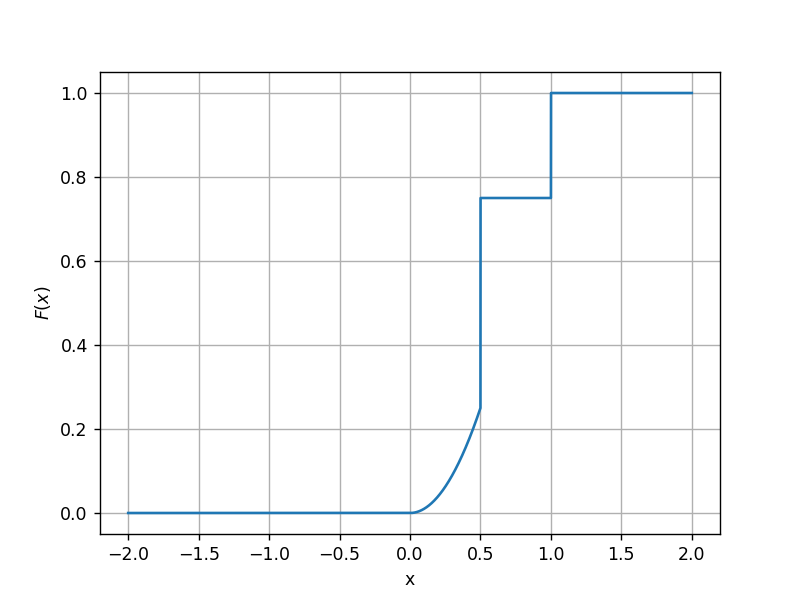
\includegraphics[width=\columnwidth]{solutions/ec/73/Assignment2.png}
\caption{The figure depicts the CDF of X}
\label{ec73:cdf}
\end{figure}



\item Let $X_1$ be an exponential random variable with mean 1 and $X_2$ a gamma random variable with mean 2 and variance 2. If $X_1$ and $X_2$ are independently distributed, then $P(X_1<X_2)$ is equal to.....

\begin{center}
\centering\underline{\textbf{Common Data for the next two Questions :}}
\end{center}

Let X and Y be two continuous random variables with the joint probability density function \\
$
f(x,y)= 
\begin{cases}
2 & 0<x+y<1, x>0, y>0 \\
0 & \text{elsewhere}.
\end{cases}
$

\item $P(X+Y<\frac{1}{2})$ is

\begin{enumerate}
\begin{multicols}{2}
\setlength\itemsep{2em}

\item $\dfrac{1}{4}$
\item $\dfrac{1}{2}$
\item $\dfrac{3}{4}$
\item 1
\end{multicols}
\end{enumerate}

\item $E(X|Y=\frac{1}{2})$

\begin{enumerate}
\begin{multicols}{2}
\setlength\itemsep{2em}

\item $\dfrac{1}{4}$
\item $\dfrac{1}{2}$
\item 1
\item 2
\end{multicols}
\end{enumerate}
%
\solution
Let X and Y be two continuous random variables with the joint probability density function 
\begin{align}
f\brak{x,y}= 
\begin{cases}
2 & 0<x+y<1, x>0, y>0 \\
0 & \text{elsewhere}.
\end{cases}   
\end{align}
\\Then $E\brak{X|Y=\frac{1}{2}}$ is 
%
Given X and Y are two continuous random variables with joint probability density function,
\begin{align}
f\brak{x,y}= 
\begin{cases}
2 & 0<x+y<1, x>0, y>0 \\
0 & \text{elsewhere}.
\end{cases}    
\end{align}
\\We know that,\\
$0<x+y<1  \implies 0<y<1-x \text{ for } 0<x<1.$\\ 
Then,
\begin{align}
    f_X\brak{x} &= \int f_{XY}\brak{x,y}dy\\
    &= \int_{0}^{1-x} (2)dy\\
    &= 2(1-x)\\
\implies f_X\brak{x} &=
    \begin{cases}
    2(1-x) & 0 \leq x <1\\
    0 & \text{otherwise}.
    \end{cases}
\end{align}
Similarly,\\
$ 0<x+y<1 \implies 0<x<1-y \text{ for } 0<y<1$ \\
Then,
\begin{align}
    f_y\brak{y} &= \int f_{XY}\brak{x,y}dx\\
    &= \int_{0}^{1-y} (2)dx\\
    &= 2(1-y)\\
\implies f_Y\brak{y} &=
    \begin{cases}
    2(1-y) & 0 \leq y <1\\
    0 & \text{otherwise}.
    \end{cases}
\end{align}
Therefore ,
\begin{align}
    f_{X|Y}\brak{x|y} &= \frac{f_{XY}\brak{x,y}}{f_Y\brak{y}}\\
    & = 
    \begin{cases}
    \frac{2}{2(1-y)} & \text{if } 0\leq x+y < 1\\
    0 & \text{otherwise}
    \end{cases}
\end{align}
Then, 
\begin{align}
   E\brak{X|Y=y} & =
   \int_{-\infty}^{\infty} (x)\brak{\frac{1}{1-y}}dx\\
    & = \frac{1}{1-y} \int_{0}^{1-y}(x)dx\\
    & = \frac{1}{1-y} \left[ \frac{x^2}{2} \right]_{0}^{1-y} \\
\therefore  E\brak{X|Y=y}& = \frac{1-y}{2}\\
\implies  E\brak{X|Y=\frac{1}{2}} & = \frac{1-\frac{1}{2}}{2}\\
\therefore E\brak{X|Y= \frac{1}{2}} &= \frac{1}{4}
\end{align}

\item If a random variable X assumes only positive integral values, with the probability \\
$
P(X=x) = \frac{2}{3}(\frac{1}{3})^{x-1}$, $x=1,2,3,...,$ \\

then $E(X)$ is

\begin{enumerate}
\begin{multicols}{2}
\setlength\itemsep{2em}

\item $\dfrac{2}{9}$
\item $\dfrac{2}{3}$
\item 1
\item $\dfrac{3}{2}$

\end{multicols}
\end{enumerate}
%
\solution
Let Y=\{0,1\} be a set of random variables of a Bernoulli's distribution with 0 representing a loss and 1 a win and let $Y_i \in Y$ for i=1,2,3...,$Y_i$ is the outcome of $i^{th}$ try of choosing 0 or 1 from Y.

 So the Random variable X is generated by assigning value of i to X where $Y_i=1$ for the first time.
\begin{align*}
&X=\{x:Y_{i=x}=1,Y_{i<x}=0\} \\
\implies & X=\{Y_1=0,Y_2=0,Y_3=0,...,Y_x=1\}
\end{align*}


For given bernouli's trail $p=\dfrac{2}{3}$ and $q=1-p=\dfrac{1}{3}$. The given probability distribution is 
\begin{align*}
&P(X=x)=P(Y_{i=x}=1)P(Y_{i<x}=0)\\
\implies &P(X=x)=p(1-p)^{x-1}\\
\implies &P(X=x)=\dfrac{2}{3}\left(\dfrac{1}{3}\right)^{x-1}
\end{align*}

The expectation value of X represented by E(X) is given by
$$E(X)=\sum_{i=1}^{\infty} Pr(x=i)\times i$$

Let S=E(X),
\begin{align}
&\implies E(X)=S=\sum_{i=1}^{\infty} Pr(x=i)\times i\\
&\implies S=\sum_{i=1}^{\infty} \dfrac{2}{3}\left(\dfrac{1}{3}\right)^{i-1} \times i \label{eq_2}   \\
&\implies S=\dfrac{2}{3}+\sum_{i=2}^{\infty} \dfrac{2}{3}\left(\dfrac{1}{3}\right)^{i-1} \times i  \label{eq_3}
\end{align}
Multiplying (\ref{eq_2}) with  $\dfrac{1}{3}$ on both sides gives
\begin{align}
&\dfrac{1}{3}S=\sum_{i=1}^{\infty} \dfrac{2}{3}\left(\dfrac{1}{3}\right)^{i} \times i \label{eq_4}
\end{align}

In (\ref{eq_3})	$\sum_{i=1}^{\infty} \dfrac{2}{3}\left(\dfrac{1}{3}\right)^{i} \times i$ can be written as $\sum_{i=2}^{\infty} \dfrac{2}{3}\left(\dfrac{1}{3}\right)^{i-1} \times (i-1)$
\begin{align}
& \implies \dfrac{1}{3}S=\sum_{i=2}^{\infty} \dfrac{2}{3}\left(\dfrac{1}{3}\right)^{i-1} \times (i-1) \label{eq_5} \\
\text{(\ref{eq_3})-(\ref{eq_5}) gives :}& \dfrac{2}{3}S=\dfrac{2}{3}+\sum_{i=2}^{\infty} \dfrac{2}{3}\left(\dfrac{1}{3}\right)^{i-1} \times (i-(i-1))\\
&\implies  \dfrac{2}{3}S=\dfrac{2}{3}+\sum_{i=2}^{\infty} \dfrac{2}{3}\left(\dfrac{1}{3}\right)^{i-1}\\
& \implies S=1+\sum_{i=1}^{\infty}\left(\dfrac{1}{3}\right)^{i}\\
& \implies S=1+\dfrac{1/3}{1-\dfrac{1}{3}}\\
& \implies S=\dfrac{3}{2} \label{eq_10}
\end{align}

The Variance Var(X) is given by $\sum x^2 P(x) - E(X)$ for the given distribution,

\begin{align}
Var(X) & =\sum_{i=1}^{\infty} i^2P(x=i) - E(X)\label{eq_11}\\
\text{let } S & = \sum_{i=1}^{\infty} i^2P(x=i)=\sum_{i=1}^{\infty} i^2 \frac{2}{3}\left(\dfrac{1}{3}\right)^{i-1} \label{eq_12}\\
S/3&= \sum_{i=1}^{\infty} i^2 \frac{2}{3}\left(\dfrac{1}{3}\right)^{i}=\sum_{i=0}^{\infty} i^2 \frac{2}{3}\left(\dfrac{1}{3}\right)^{i}\\
& = \sum_{i=1}^{\infty} (i-1)^2 \frac{2}{3}\left(\dfrac{1}{3}\right)^{i-1}\label{eq_14}
\end{align}

(\ref{eq_12})-(\ref{eq_14}) gives us
\begin{align}
\dfrac{2S}{3} & = \sum_{i=1}^{\infty} (i^2-(i-1)^2) \frac{2}{3}\left(\dfrac{1}{3}\right)^{i-1}\\
S &= \sum_{i=1}^{\infty} (2i-1)\left(\dfrac{1}{3}\right)^{i-1} \\
\implies S&= 3 \sum_{i=1}^{\infty} \frac{2}{3}\left(\dfrac{1}{3}\right)^{i-1}i-\sum_{i=1}^{\infty} \left(\dfrac{1}{3}\right)^{i-1} \\
\implies S&= 3E(X)-\dfrac{1}{1-1/3}\\
\implies S& = \frac{9}{2}-\frac{3}{2}=3 \label{eq_19}
\end{align}

From (\ref{eq_19}) and (\ref{eq_11}) we can write 
$$Var(X)=3-\frac{3}{2}=\frac{3}{2}$$

From (\ref{eq_10}) we can say that the expectation value of X given by E(X)=S=$\dfrac{3}{2}$		
and $Var(X)=\dfrac{3}{2}$  



\item The joint probability density function of two random variables X and Y is given as \\
$
f(x,y)=
\begin{cases}
\dfrac{6}{5}(x+y^2)
& 0 \leqslant x \leqslant 1  0 \leqslant x \leqslant 1 \\
0 & \text{elsewhere}
\end{cases}
$\\
$E(X)$ and $E(Y)$ are, respectively,

\begin{enumerate}
\begin{multicols}{2}
\setlength\itemsep{2em}

\item $\dfrac{2}{5}$ and $\dfrac{3}{5}$
\item $\dfrac{3}{5}$ and $\dfrac{3}{5}$
\item $\dfrac{3}{5}$ and $\dfrac{6}{5}$
\item $\dfrac{4}{5}$ and $\dfrac{6}{5}$
\end{multicols}
\end{enumerate}
%
\solution
For a continuous joint probability distribution  $\e{X}$ \\
and $\e{Y}$ are obtained using the following equations  \\
\eqref{ec78:a} and \eqref{ec78:b}
\begin{align}
\e{X} &= \Int_{-\infty}^{+\infty}\Int_{-\infty}^{+\infty} x \cdot \fn{x,y}\,dx\,dy \label{ec78:a} \\ 
\e{Y} &= \Int_{-\infty}^{+\infty}\Int_{-\infty}^{+\infty} y \cdot \fn{x,y}\,dx\,dy \label{ec78:b}
\end{align}
Using equation \eqref{ec78:a} \e{X} is calculated as 
\newpage
\begin{align*}
\e{X} &= \Int_{0}^{1}\Int_{0}^{1} x\,\dfrac{6}{5}\brak{x+y^2}\,dx\,dy \;+ 0 \\ 
      &= \Int_{0}^{1}\dfrac{6}{5}\brak{\Int_{0}^{1}x^2\,dx}+\dfrac{6}{5}\,y^2\,\brak{\Int_{0}^{1}x\,dx}\;dy   \\
      &= \Int_{0}^{1}\dfrac{6}{5}\brak{\dfrac{1}{3}}+\dfrac{6}{5}\,y^2\,\brak{\dfrac{1}{2}}\;dy \\
      &= \dfrac{2}{5}\Int_{0}^{1}\,dy + \dfrac{3}{5}\Int_{0}^{1}y^2\,dy  \\
      &= \dfrac{2}{5} + \dfrac{3}{5}\brak{\dfrac{1}{3}} \\
\e{X} &=  \dfrac{3}{5}  
\end{align*}
Using equation \eqref{ec78:b} \e{Y} is calculated as
\begin{align*}
\e{Y} &= \Int_{0}^{1}\Int_{0}^{1} y\,\dfrac{6}{5}\brak{x+y^2}\,dx\,dy \;+ 0 \\ 
      &= \Int_{0}^{1}\dfrac{6}{5}\,x\brak{\Int_{0}^{1}y\,dy} + \dfrac{6}{5}\brak{\Int_{0}^{1}y^{3}\,dy}\;dx \; \\ 
      &= \Int_{0}^{1}\dfrac{6}{5}\,x\brak{\dfrac{1}{2}} + \dfrac{6}{5}\brak{\dfrac{1}{4}}\;dx \; \\ 
      &= \dfrac{3}{5}\Int_{0}^{1}x\,dx\;+\;\dfrac{3}{10}\Int_{0}^{1}\,dx  \\
      &= \dfrac{3}{5} \brak{\dfrac{1}{2}} + \dfrac{3}{10} \\
\e{Y} &= \dfrac{3}{5}      
\end{align*}
 $$\therefore \e{X} = \dfrac{3}{5}\;\text{and}\;\e{Y} = \dfrac{3}{5}$$ 
 Hence the answer is \textbf{option b}

\item Suppose the random variable U has uniform distribution on $[0,1]$ and $X= -2 \log U$. The density of X is \\

\begin{enumerate}
\setlength\itemsep{2em}

\item $
f(x)=
\begin{cases}
e^{-x} &  x>0\\
0 & \text{otherwise}
\end{cases}
$

\item $
f(x)=
\begin{cases}
2e^{-2x} &  x>0 \\
0 & \text{otherwise}
\end{cases}
$

\item $
f(x)=
\begin{cases}
\dfrac{1}{2}e^-{\frac{x}{2}} &  x>0 \\
0 & \text{otherwise}
\end{cases}
$

\item $
f(x)=
\begin{cases}
\dfrac{1}{2} &  x \in [0,2] \\
0 & \text{otherwise}
\end{cases}
$

\end{enumerate}
\solution
$U$ - uniformly distributed random variable on $\in$ [0,1]. 
Probability density function of $U$ is: 
\begin{align}
    f_U(u) =
    \begin{cases}
     1  & x \in  [0,1] \\
    0 & \text{otherwise} 
    \end{cases}
\end{align}
 $X$ is given by :
\begin{align}
  X = -2 \ln(U) \\
\implies    0 \leq X \leq \infty
\end{align}
CDF of  $X$ is defined as 
\begin{align}
    F_X(x) &= \pr{X \le x} \\
           &= \pr{-2 \ln(U)\le x} \\
           &= \pr{\ln(U) \ge( -x) /2}\\
           &= \pr {U \ge \exp(-x/2)}\\
           &= 1 - \pr{U \le exp(-x/2)}\\
           &= 1 - exp(-x/2) 
\end{align}
where x $\in$ [0,$\infty$] \\
PDF of $X$ : 
\begin{align}
    f_X(x) & = \frac{d (F_X (x)) }{dx} \\
           & = \frac{1}{2}  exp((-x)/2)
\end{align}
 we have     
\begin{align}
    0 \leq X \leq \infty
\end{align}
\begin{align}
    f_X(x) =
    \begin{cases}
    \frac{1}{2}  exp(\frac{-x}{2}) & x > 0 \\
    0 & \text{otherwise}
    \end{cases}
\end{align}
$\therefore$ answer will be option \brak 3


\item Suppose X is a real-valued random variable. Which of the following values CANNOT be attained by $E[X]$ and $E[X^2]$, respectively?

\begin{enumerate}
\begin{multicols}{2}
\setlength\itemsep{2em}

\item 0 and 1
\item 2 and 3
\item $\dfrac{1}{2}$ and $\dfrac{1}{3}$
\item 2 and 5
\end{multicols}
\end{enumerate}
\solution
The variance of a distribution is given by
\begin{align}
    \sigma^2 %&= \sum_{X \in \mathbb{R}} \left(  (E\left[ X-E[X] \right])^2 \pr{X} \label{varience} \right)\\
    = E[X^2] - E[X]^2
\end{align}
As variance is always positive, 
\begin{align}
    E[X^2] - E[X]^2 \geq 0
\end{align}
is a necessary condition for any real valued random variable. Computing the value of $E[X^2] - E[X]^2$ for the options, we have
\begin{enumerate}[label=(\Alph*)]
\setlength\itemsep{2em}
\item 0 and 1
\begin{align}
    \implies E[X^2] - E[X]^2 = 1 -0^2 = 1 \geq 0
\end{align}
\item 2 and 3
\begin{align}
    \implies E[X^2] - E[X]^2 =3 -2^2 =-1 \leq 0 \label{negative_variance}
\end{align}
\item $\dfrac{1}{2}$ and $\dfrac{1}{3}$
\begin{align}
    \implies E[X^2] - E[X]^2 = \frac{1}{3} - \frac{1}{2}^2 = \frac{1}{12}\geq 0
\end{align}
\item 2 and 5
\begin{align}
    \implies E[X^2] - E[X]^2 = 5 -2^2 = 1 \geq 0
\end{align}
\end{enumerate}

\item Probability density function $p(x)$ of a random variable x is as shown below. The value of $\alpha$ is 

\begin{figure}[!h]
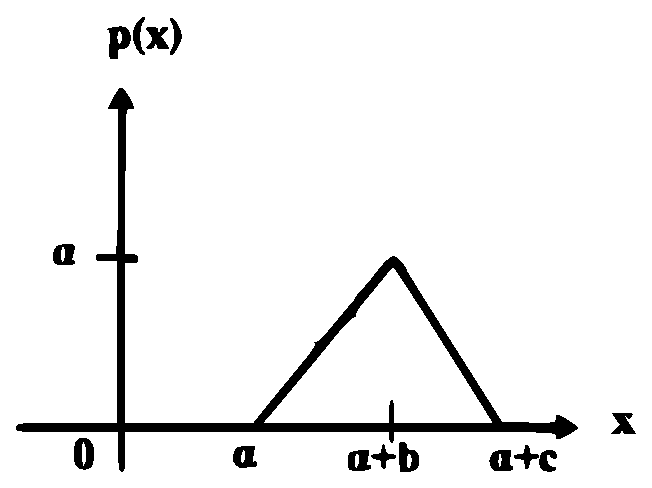
\includegraphics[width=\columnwidth]{./figs/figure13.eps}
\caption{}
\label{fig:13}
\end{figure}


\begin{enumerate}
\begin{multicols}{2}
\setlength\itemsep{2em}

\item $\dfrac{2}{c}$
\item $\dfrac{1}{c}$
\item $\dfrac{2}{(b+c)}$
\item $\dfrac{1}{(b+c)}$

\end{multicols}
\end{enumerate}

\item A player throws a ball at a basket kept at a distance. The probability that the ball falls into the basket in a single attempt is 0.1. The player attempts to throw the ball twice. Considering each attempt to be independent, the probability that this player puts the ball into the basket only in the second attempt is.........
\\
\solution
Let $X\in\mathbb{N}$ represent the number of times the experiment is performed. \\
$X=k$ represents $k-1$ failures were obtained before getting 1 success. $p$ represents the probability of success
\begin{align}
	p_X(k) &=
\begin{cases}
\brak{1-p}^{k-1}\times p & k\in \mathbb{N}\\
0 &  otherwise 
\end{cases}
\label{2020:eq:final_result}
\end{align}
Using \eqref{2020:eq:final_result} we get
\begin{align}
\pr{X=2}&=\brak{1-p}^{k-1}\times p\nonumber\\
&=\brak{0.9}\times 0.1=0.09
\end{align}
\item A screening test is carried out to detect a certain disease. It is found that $12\%$ of the positive
reports and $15\%$ of the negative reports are incorrect. Assuming that the probability of a
person getting positive report is 0.01, the probability that a person tested gets an incorrect
report is \dots
\\
\solution
Let $X \in \{0,1\}$ represent the random variable, where 0 represents the case where a person gets a positive report while 1 represents the case where a person gets a negative report. From the question, 
\begin{align}
    \Pr{(X=0)} = 0.01
    \\\Pr{(X=0)} + \Pr{(X=1)} = 1
    \\\Pr{(X=1)} = 1 - 0.01 = 0.99
\end{align}
Let $Y \in \{0,1\}$ represent the random variable, where 0 represents a correct report whereas 1 represents an incorrect report.

\begin{align}
    \Pr{(Y=1 | X=0)} = 12\% = 0.12
    \\\Pr{(Y=1 | X=1)} = 15\% = 0.15
\end{align}
Then, from total probability theorem,
\begin{multline}
    \Pr{(Y=1)} = \Pr{(Y=1, X=0)} 
    \\+ \Pr{(Y=1, X=1)}
\end{multline}
Using Bayes theorem,
\begin{multline}
    \Pr{(Y=1)} = \Pr{(Y=1 | X=0)} \times \Pr{(X=0)}
    \\ + \Pr{(Y=1 | X=1)} \times \Pr{(X=1)}
\end{multline}
    
\begin{align}
    \Pr{(Y=1)} = & 0.12 \times 0.01 + 0.15 \times 0.99
    \\ = & 0.0012 + 0.1485
    \\ = & 0.1497    
\end{align}
%
\item Shaquille O’ Neal is a 60\% career free throw shooter, meaning that he successfully makes 60 free throws out of 100 attempts on average. What is the probability that he will successfully make exactly 6 free throws in 10 attempts?
\begin{enumerate} [label={\Alph*)}]
\item 0.2508
\item 0.2816
\item 0.2934
\item 0.6000
\end{enumerate}
%
\solution
Let 
\begin{align}
X_{i}\in \{0,1\}
\end{align}
represent the $i^{th}$ free throw, where 1 represents a successful free throw attempt and 0 represents an unsuccessful attempt.
Let
\begin{align}
X=\sum_{i=1}^{n} X_{i}   
\end{align}
where n is the total number of free throws. Then, X has a binomial distribution with
\begin{align}
\pr {X=k}=\comb{n}{k} p^{k} q^{n-k}
\end{align}
Where,
\begin{align}
  &p=\frac{6}{10}\\
  &q=1-p=\frac{4}{10}\\
  &n=10
\end{align}
from the given information. Then,
\begin{align}
\pr{X=6}&=\comb{10}{6}\brak{\frac{6}{10}}^{6}\brak{\frac{4}{10}}^{4}
\end{align}
On simplifying we get,
\begin{align}
\pr{X=6}&=0.2508
\end{align}
Therefore, the probability that he will successfully make exactly 6 free throws in 10 attempts is 0.2508 and hence option (A) is correct.
%
\item  Consider a sequence of tossing a fair coin where outcomes of tosses are independent.The probability of getting the head for the third time in the fifth toss is
    \begin{enumerate}[label=(\Alph*)]
      \item $\dfrac{5}{16}$  \item $\dfrac{3}{16}$ \item $\dfrac{3}{5}$ \item $\dfrac{9}{16}$
    \end{enumerate}
    \solution
Let the random variable $X \in \{0,1\}$ denotes head and tail in a toss.As both are equally probable.
\begin{align}
    \pr{X=0}=\dfrac{1}{2}\\
    \pr{X=1}=\dfrac{1}{2}
\end{align}

\begin{table}[h]
\begin{tabular}{|c|c|}
\hline
\textbf{Event} & \textbf{Description}                 \\ \hline
A              & nth toss is a head                   \\ \hline
B              & Exactly k-1 heads in first four tosses \\ \hline
C              & nth toss is the third head           \\ \hline
\end{tabular}
\caption{Description of events used in problem}
\label{tab:Events}
\end{table}

\begin{align}
\pr{A}&=\pr{X=1}=\dfrac{1}{2}\\
\pr{B}&=\dfrac{{}^{n-1}C_{k-1}}{2^{n-1}}
\end{align}

\begin{align}
    C&=AB\\
    \pr{C}&=\pr{AB}
\end{align}
As A and B are independent events.
\begin{align}
    \pr{C}&=\pr{A}\pr{B}\\
    &=\dfrac{1}{2}\times\dfrac{{}^{n-1}C_{k-1}}{2^{n-1}}\\
    &=\dfrac{{}^{n-1}C_{k-1}}{2^n}
\end{align}
Here n=5,k=3
\begin{align}
    \pr{C|n=5,k=2}&=\dfrac{{}^{4}C_{2}}{2^{5}}\\
    &=\dfrac{6}{32}
\end{align}

Therefore probability of getting the head for the third time in the fifth toss is $\dfrac{3}{16}$. 


\item A random variable $X$ takes values -1 and +1 with probabilities 0.2 and 0.8, respectively.
It is transmitted across a channel which adds noise $N$, so that the random variable at the
channel output is $Y = X + N$. The noise $N$ is independent of $X$, and is uniformly
distributed over the interval [-2 , 2]. The receiver makes a decision
\[
\hat{X} = \begin{cases}
            -1, &\text{if}\quad Y \leq \theta \\
             +1, &\text{if}\quad Y \geq \theta\\
            \end{cases}
\]
where the threshold $\theta  \in [-1,1]$ is chosen so as to minimize the probability of error
\pr {\hat{X} \neq X}. The minimum probability of error, rounded off to 1 decimal place, is \dots
\\
\solution

We know that 
\begin{align}
    X \in \{-1,+1\}\\
    N \in [-2,2]\\
    Y = X + N\\
    \pr{X = -1} = 0.2\\
    \pr{X = +1} = 0.8
\end{align}
Since $N$ is uniformly distributed\\
$\therefore$ the probability distribution function of $N$ is:

\begin{tikzpicture}[
  declare function={
    func(\x)= (\x < -2) * (0)   +
              and(\x >= -2, \x < 2) * (0.25)     +
              (\x >= 2) * (0)
   ;
  }
]
\begin{axis}[
  axis x line=middle, axis y line=middle,
  ymin=0, ymax=1, ytick={0,0.25,0.5,0.75,1}, ylabel=$f(N)$,
  xmin=-3, xmax=3, xtick={-3,...,3}, xlabel=$N$,
  domain=-3:3,
  samples=100,
]

\addplot [blue,thick] {func(x)};
\end{axis}
\end{tikzpicture}
\\
The cdf of this uniform probability distribution function is
\begin{align}
    F_X(x) &= \int_{-\infty}^xf(N)dN \\ 
    &=\int_{-2}^x\frac{1}{4}dN\\
    &=\frac{x+2}{4}\label{eq:0.0.8}
\end{align}
For $X \neq \hat{X}$ we need to check for each case. Using equation \eqref{eq:0.0.8}
\begin{align}
\therefore
    \pr{N>\theta + 1} &= 1-\pr{N < \theta + 1}\\
    &= 1-F_X(\theta + 1)\\
    &= 1- \frac{\theta + 3}{4}\\
    &= \frac{1}{4}(1-\theta)\label{eq:0.0.12}
\end{align}
\begin{align}
\therefore
    \pr{N < \theta-1} &= F_X(\theta - 1)\\
    &= \frac{1}{4}(1+\theta)\label{eq:0.0.14}
\end{align}
The probability of error:
\begin{align}
\nonumber
    \pr {\hat{X} \neq X} = P(-1)\cdot {P(\theta < -1 + N)} \\ 
            \quad+ P(1)\cdot {P(\theta> N + 1)}\label{eq:0.0.15}
\end{align}
Substituting \eqref{eq:0.0.12} and \eqref{eq:0.0.14} in \eqref{eq:0.0.15}. We get:
\begin{align}
\nonumber
    \pr {\hat{X} \neq X} &= 0.2\cdot \frac{1}{4}(1-\theta) \\
    & \quad+ 0.8\cdot \frac{1}{4}(1+\theta)
\end{align}
On simplifying the equation we get
\begin{align}
    \pr {\hat{X} \neq X} = \frac{1}{4} + \frac{3}{20}\theta
\end{align}
Since this is a linear equation in $\theta$, the minimum will occur at boundary points.
Putting $\theta = +1$, we get
\begin{align}
    \pr {\hat{X} \neq X} = 0.4
\end{align}
but on putting $\theta = -1$, we get
\begin{align}
    \pr {\hat{X} \neq X} = 0.1
\end{align}
Hence the value of probability of error is:
\begin{align}
    \therefore \pr {\hat{X} \neq X} = 0.1
\end{align}


\item You have gone to a cyber-cafe with a friend. You found that the cyber-café has only three terminals. All terminals are unoccupied. You and your friend have to make a random choice of selecting a terminal. What is the probability that both of you will NOT select the same terminal?
%
\\
\solution
There are three terminals, each with an equal 
\begin{math}
\\\text{probability of }\frac{1}{3} \text{ to be picked.}
\\\text{Defining random variables }X_1, X_2\in\cbrak{0, 1, 2}
\\\text{Where,}
\\X_i = 0 \text{ when ith man picks first terminal.}
\\X_i = 1 \text{ when ith man picks second terminal.}
\\X_i = 2 \text{ when ith man picks third terminal.}
\end{math}
\begin{align}
    \pr{X_1 \ne X_2} &= 1 - \pr{X_1 = X_2}.
    \\\implies \pr{X_1 = X_2} &= \sum_{j=1}^3 \pr{X_1 = X_2 = j} 
    \\\implies\pr{X_1=X_2}&=\sum_{j=1}^3\brak{{\frac{1}{3}}\times{\frac{1}{3}}} = {\frac{1}{3}}
\end{align}
\begin{align}
    \therefore \pr{X_1 \ne X_2} = \frac{2}{3}.
\end{align}


\item A sender(S) transmits a signal,which can be one of two kinds: H and L with probabilities 0.1 and 0.9 respectively, to a receiver (R).\\
In the graph below,the weight of an edge(u,v) is the probability of receiving v when u is transmitted,where u,v $\in$ \{H,L\}.For example the probability that the received signal is L given the transmitted signal is H is 0.7.
\begin{figure}[h!]
    \centering
    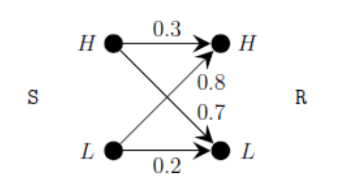
\includegraphics[width=\columnwidth]{solutions/cs/2021/figures/qnfigure.png}
\end{figure}
%
If the received signal is H, the probability that the transmitted signal was H is \underline{\quad\quad\quad} ?

\solution


%
In our problem we have a binary channel which is not symmetric as crossover probabilities differ\\
Let $A \in \{0,1\}$ represent the random variable, where 0 represents H being transmitted, 1 represents L being transmitted. \\
Let $B \in \{0,1\}$ represent the random variable, where 0 represents H being received, 1 represents L being received. \\
\begin{table}[ht]
\caption{Probability for random variables}
\centering
\resizebox{\columnwidth}{!}{
\begin{tabular}{|c|c|c|c|}
\hline
{\pr{A=0}}&0.1  &{\pr{A=1}}& 0.9  \\ \hline
\pr{B=0|A=0}&  0.3 &\pr{B=0|A=1}& 0.8 \\ \hline
{\pr{B=1|A=0}}& 0.7 &\pr{B=1|A=1}& 0.2  \\ \hline 
\end{tabular}
}
\label{Tab:Tcr}
\end{table}
\\
Now we need to find \pr{A=0|B=0}\\
Using Bayes theorem
\begin{align}
\pr{A=0|B=0}=\frac{\pr{A=0}\times\pr{B=0|A=0}}{\sum_{i=0}^1 \pr{A=i} \times\pr{B=0|A=i}}
\end{align}
Putting in values given in question
\begin{align}
   \pr{A=0|B=0}=\frac{1}{25}=0.04 
\end{align}
The probability that transmitted signal was H is 0.04 


\item A box has ten light bulbs out of which two are defective, Two light bulbs are drawn from this box one after the other without replacement. The probability that both light bulbs drawn are not defective is 
\begin{enumerate}[label={\Alph*)}]
\begin{multicols}{4}
\setlength\itemsep{2em}
\item $\dfrac{8}{45}$
\item $\dfrac{28}{45}$
\item $\dfrac{16}{25}$
\item $\dfrac{4}{5}$
\end{multicols}
\end{enumerate}
\solution
Let $X_i \in \cbrak{0,1}$ represent the $i^{th}$ draw, where 0 denotes a defective bulb and 1 denotes a non-defective bulb.
\begin{table}[h]
\centering 
\caption{}
\begin{tabular}{|c|c|c|}
\hline
           & $X_1 = 0$ & $X_1 = 1$\\
\hline
$X_2 = 0$  & 2/90      & 16/90  \\
\hline
$X_2 = 1$  & 16/90      & 56/90  \\
\hline
\end{tabular}
\label{xe2015:table}
\end{table}
 
Table \ref{table} represents the probabilities of all possible cases when two bulbs are drawn one by one without replacement.
Probability that both of the bulbs are non-defective (by substituting values from table \ref{table})
\begin{align}
    &= \Pr\brak{X_2 = 1|X_1 = 1}\Pr\brak{X_1 = 1}\\
    &= \dfrac{56}{90}\\
    &= \dfrac{28}{45}
\end{align}
So the correct option is (B)
%
\item Three fair dies are rolled simultaneously. The probability of getting a sum of 5 is
\begin{enumerate}
    \item $\frac{1}{108}$
    \item $\frac{1}{72}$
    \item $\frac{1}{54}$
    \item $\frac{1}{36}$
\end{enumerate}
%
\solution


Let
$X_i\in\,$\cbrak{1,2,3,4,5,6}, i = 1,2,3, be the random variables representing the outcome for each die. As the dies are fair, the probability mass function (pmf) is expressed as
\begin{align}
    p_{X_i}(n) = \pr{X_i = n} = 
\begin{cases}
\frac{1}{6} & 1 \le n \le 6
\\
0 & otherwise
\end{cases}\label{1}
\end{align}
Let X be a random variable denotes the desired outcome,
\begin{align}
    X=X_1+X_2+X_3\label{2}\\
    \implies X\in\cbrak{3,4,\cdots,18}
\end{align}

We have to find $P_X(n)$ = $\pr{X_1+X_2+X_3=n}$
\begin{multline}
    p_X(n)=\pr{X_1+X_2+X_3=n}\\
   =\pr{X_1+X_2=n-X_3}\\
    =\Sigma_{k}{\pr{X_1+X_2=n-k|X_3=k}p_{X_3}(k)}\label{3}
\end{multline}
As $X_1,X_2,X_3$ are independent, After unconditioning
\begin{align}
    \pr{X_1+X_2=n-k|X_3=k}=\pr{X_1+X_2=n-k}\label{6}
\end{align}
Using \eqref{6} in \eqref{3}
\begin{multline}
    p_X(n)=\Sigma_{k}{\pr{X_1+X_2=n-k|X_3=k}p_{X_3}(k)}\\
    =\Sigma_{k}{\pr{X_1+X_2=n-k}p_{X_3}(k)}\\
    =\Sigma_{k}{\brak{\Sigma_{a}{\pr{X_1=n-k-a|X_2=a}\pr{X_2=a}}}p_{X_3}(k)}\\
    =\Sigma_{k}{\brak{\Sigma_{a}{\pr{X_1=n-k-a}\pr{X_2=a}}}p_{X_3}(k)}\\
    =\Sigma_{k}{\brak{\Sigma_{a}{p_{X_1}\brak{n-k-a}p_{X_2}\brak{a}}}p_{X_3}(k)}\label{4}
\end{multline}
Equation \eqref{4} can be written as follows using convolution operation,
\begin{align}
    \nonumber p_X(n)&=\Sigma_{k}{\brak{\Sigma_{a}{p_{X_1}\brak{n-k-a}p_{X_2}\brak{a}}}p_{X_3}(k)}\\
    &=p_{X_1}\brak{n}*p_{X_2}\brak{n}*p_{X_3}\brak{n}\label{5}
\end{align}
The Z-transform of $p_X(n)$ is defined as
\begin{align}
P_X(z) = \sum_{n = -\infty}^{\infty}p_X(n)z^{-n}, \quad z \in \mathbb{C}
\label{7}
\end{align}
%
From \eqref{1} and \eqref{7}, 
\begin{align}
\nonumber P_{X_1}(z) =P_{X_2}(z)&=P_{X_3}(z)\\
&= \frac{1}{6}\sum_{n = 1}^{6}z^{-n}
\\
&=\frac{z^{-1}\brak{1-z^{-6}}}{6\brak{1-z^{-1}}}, \quad \abs{z} > 1
\label{8}
\end{align}
upon summing up the geometric progression. 
From \eqref{5},
\begin{align}
\because p_X(n) &= p_{X_1}(n)*p_{X_2}(n)*p_{X-3}(n),
\\
P_X(z) &= P_{X_1}(z) P_{X_2}(z)P_{X_3}(z)
\label{9}
\end{align}
The above property follows from Fourier analysis and is fundamental to signal processing.\\
From \eqref{8} and \eqref{9},
\begin{align}
    P_X{\brak{z}}&=\cbrak{\frac{z^{-1}\brak{1-z^{-6}}}{6\brak{1-z^{-1}}}}^3\\
    &= \frac{1}{216}\frac{z^{-3}\brak{1-3z^{-6}+3z^{-12}-z^{-18}}}{\brak{1-z^{-1}}^3}\label{10}
\end{align}
Using the fact that,
\begin{align}
p_X(n-k) &\system{Z}P_X(z)z^{-k},
\\
nu(n)&\system{Z} \frac{z^{-1}}{\brak{1-z^{-1}}^2}\\
n^2u(n)&\system{Z} \frac{z^{-1}\brak{1+z^{-1}}}{\brak{1-z^{-1}}^3}\\
(n^2+n)u(n)&\system{Z} \frac{2z^{-1}}{\brak{1-z^{-1}}^2}
\end{align}
after some algebra, it can be shown that,
\begin{multline}
\frac{1}{216\times 2}\lsbrak{\brak{(n-2)^2+n-2}u(n-2)} \\-3 \brak{(n-8)^2+n-8}u(n-8)\\+3\brak{(n-14)^2+n-14}u(n-14)\\-\rsbrak{\brak{(n-20)^2+n-20}u(n-20)}
\\
\system{Z}
\frac{1}{216}\frac{z^{-3}\brak{1-3z^{-6}+3z^{-12}-z^{-18}}}{\brak{1-z^{-1}}^3}
\label{11}
\end{multline}
where 
\begin{align}
u(n) =
\begin{cases}
1 & n \ge 0
\\
0 & n < 0\label{13}
\end{cases}
\end{align}
From \eqref{7},\eqref{10} and \eqref{11},
\begin{multline}
p_{X}(n) = \frac{1}{216\times 2}\lsbrak{\brak{(n-2)^2+n-2}u(n-2)} \\-3 \brak{(n-8)^2+n-8}u(n-8)\\+3\brak{(n-14)^2+n-14}u(n-14)\\-\rsbrak{\brak{(n-20)^2+n-20}u(n-20)}
\label{12}
\end{multline}
From \eqref{13} and \eqref{12},
\begin{align}
p_X(n) &= 
\begin{cases}
0 & n < 3\\
\frac{n^2-3n+2}{432} &  3 \le n \le  8\\
\frac{42n-2n^2-166}{432} & 8 < n \le 14\\
\frac{n^2-39n+380}{432} & 14 < n \le 18\\
0 & n > 18\label{14}
\end{cases}
\end{align}
\begin{figure}[htp]
    \centering
    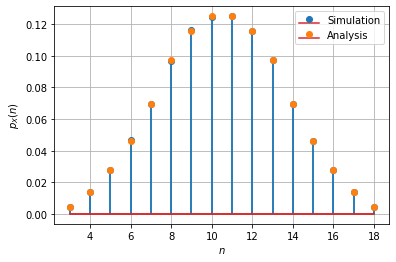
\includegraphics[width=\columnwidth]{solutions/xe/2017/figures/assign3_stem.png}
    \caption{Probability mass function of X}{ (simulations are close to analysis)}
\end{figure}
We need probability of getting sum of 5,\\$\implies$ n=5 \\from \eqref{14} and using n=5,
\begin{align}
    p_X(5)&=\frac{5^2-3(5)+2}{432}\\
    p_X(5)&=\frac{12}{432}\\
    p_X(5)&=\frac{1}{36}
\end{align}

Therefore the probability of getting a sum of 5 when three fair dies are rolled is $\frac{1}{36}$.\\
\textbf{Ans: Option (D)}


\item What is the chance that a leap year,selected at random,will contain 53 Saturdays? \\
\begin{enumerate}
    \item  $\frac{2}{7}$ 
    \item  $\frac{3}{7}$ 
    \item  $\frac{1}{7}$ 
    \item  $\frac{5}{7}$ 
\end{enumerate}
\solution
\input{solutions/ee/2013.tex}
%
\item Let $\mathcal{R}$  be the set of all binary relations on the set $\{1,2,3\}$. Suppose a relation is chosen from $\mathcal{R}$ at random. The probability that the chosen relation is reflexive is?
\\
\solution
Let $A$ be a set of n numbers. No. of pairs formed from elements of $A$:\\
\begin{align}
     \comb{n}{1} \times \comb{n}{1} = n^2\label{cs2020:eq1}
\end{align}
\\For each pair we have 2 choices, whether to include it in the relation or not. \\$\therefore$ Number of binary relations on $A$:\\
\begin{align}
    2\times2\times...\text{ $n^{2}$ times } = 2^{n^2}\label{cs2020:eq2}
\end{align}
\begin{definition}
A reflexive relation is one in which every element maps to itself, i.e., a relation $R$ on set $A$ is reflexive if $(a,a) \in R\; \forall\; a \in A$.
\end{definition}
For example, consider the set $A$\hspace{0.2cm}=\hspace{0.2cm}$\{1,2,3\}$. A possible reflexive relation on $A$ is $R_1$\hspace{0.2cm}=\hspace{0.2cm}$\{(1,1), (2,2), (3,3), (1,2), (2,3)\}$ as every element in $A$ is related to itself in $R_1$ while relation $R_2$\hspace{0.2cm}=\hspace{0.2cm}$\{(1,1),(2,2),(1,2)\}$ is not a reflexive relation on $A$ as 3 $\in A$ but $(3,3) \notin R_2$.\\
In a reflexive relation, out of the $n^2$ pairs \eqref{eq1}, n have to be included (n pairs of the form (a,a)) which means there is only 1 way to include them. For the remaining $n^2-n$ pairs we have 2 choices, whether to include it in the relation or not.\\
$\therefore$ Number of reflexive relations are:\\
\begin{align}
    1\times2^{n^{2}-n} = 2^{n^{2}-n} \label{cs2020:eq3}
\end{align}
\\
Let $X \in \{0,1\}$ be a random variable where 0 represents reflexive relation chosen from $\mathcal{R}$ and 1 represents non-reflexive relation chosen from $\mathcal{R}$. In this case, n=3.
\\
\begin{align}
    \pr{X=0} &= \frac{2^{n^{2}-n}}{2^{n^{2}}} \nonumber\\
    &= \frac{2^{6}}{2^{9}}\\
    \therefore \text{ Answer }= \frac{1}{8}
\end{align}

%
\item If P and Q are two random events, then the following is true:
\begin{enumerate}[label = (\alph*)]
    \item Independence of P and Q implies that probability $(P\cap Q)=0 $ 
    \item Probability $(P\cup Q) \leq   $ Probability $(P)$ + Probability(Q) 
    \item If P and Q are mutually exclusive, then they must be independent
    \item Probability $(P\cap Q) \leq$ Probability $(P)$
\end{enumerate}
%
\solution
For two random events A and B that are independent, we know that, 
\begin{align}
Pr(AB) = Pr(A)Pr(B)
\end{align}
and for two mutually exclusive events C and D, 
\begin{align}
    Pr(CD) = 0
\end{align}

\begin{enumerate}[label = (\alph*)]
    \item Independence of P and Q implies that the occurrence of one is unaffected by the other. 
    \begin{align}
       \Rightarrow Pr(PQ) = Pr(P)Pr(Q)
    \end{align}
    The given option will be true only when either Pr(P) or Pr(Q) will be zero, therefore, (a) is incorrect.\\
    \item From set theory,
    \begin{align}
    A\cup B &= A + B - A\cap B
    \end{align}
    \begin{multline}
    \Rightarrow Pr(P+Q) = Pr(P) \\+ Pr(Q)- Pr(PQ)
    \label{ee2005:eq:5}
    \end{multline}
    \begin{align}
    \Rightarrow Pr(P+Q) &\leq Pr(P) + Pr(Q)
    \end{align}
    thus, (b) is incorrect.\\
    \item Two events can be both mutually exclusive and independent only when one of them have a zero probability. Since it isn't necessary that $Pr(P)=0$ or $Pr(Q)=0$, (c) is incorrect.\\
    \item The set $P$ will have either have the same or more elements than the set $P\cap Q$
    \begin{equation}
        Pr(PQ) \leq Pr(P)
    \end{equation}
    (d) is correct.\\
\end{enumerate}
Thus, the only correct option is (d).
%
\item A diagnostic test for a certain disease is 90\% accurate. That is, the probability of a person having (respectively, not having) the disease tested positive (respectively, negative) is 0.9. Fifty percent of the population has the disease. What is the probability that a randomly chosen person has the disease given that the person tested negative?
\\
\solution
Let X and Y be two Bernoulli random variables such that X,Y$\in$\cbrak{0,1} and as given fifty percent of the population has the disease, the probability mass function of X is 
\begin{align}
    p_{X}(n) = \pr{X = n} = 
\begin{cases}
0.5 &  n=1
\\
0.5 & n=0
\\
0 & otherwise
\end{cases}\label{xe2016-8:1}
\end{align}
where X denotes the health status of a person(X=1 if person is healthy and X=0 if person is diseased) and Y denotes the diagnostic test result (Y=1 if it is positive and Y=0 if it is negative).
\\Given the probabilities of,
\begin{align}
    \pr{Y=1|X=0}=0.9\label{xe2016-8:2}
    \\\pr{Y=0|X=1}=0.9 \label{xe2016-8:3}
\end{align}
we need to find $\pr{X=0|Y=0}$,
\begin{align}
    \pr{X=0|Y=0}&=\frac{\pr{X=0\cap Y=0}}{\pr{Y=0}}\\
    \pr{X=0|Y=0}&=\frac{\pr{Y=0|X=0}\pr{X=0}}{\pr{Y=0}}\label{xe2016-8:4}
\end{align}
\begin{multline}
    \pr{Y=0}=\pr{Y=0|X=1}\pr{X=1}\\+\pr{Y=0|X=0}\pr{X=0}\label{xe2016-8:5}
\end{multline}
Using \eqref{xe2016-8:1},\eqref{xe2016-8:2} and \eqref{xe2016-8:3} in \eqref{xe2016-8:5},
\begin{align}
    \nonumber\pr{Y=0}&=0.9(0.5)+(1-0.9)0.5\\
    \pr{Y=0}&= 0.5\label{xe2016-8:6}
\end{align}
Using \eqref{xe2016-8:1},\eqref{xe2016-8:2} and \eqref{xe2016-8:6} in \eqref{xe2016-8:4}
\begin{align}
    \pr{X=0|Y=0}&=\frac{(1-0.9)0.5}{0.5}\\
    \pr{X=0|Y=0}&= 0.1
\end{align}
%
\item Box-S has $2$ white and $4$ black balls and box-T has $5$ white and $3$ black balls.A ball is drawn at \\ random from box-S and put in box-T.Subsequently,the probability of drawing a white ball from box-T is? (rounding off to $ 2 $ decimal places)
%
\\
\solution
Box-0 has $2$ white and $4$ black balls.\\
Box-1 has $5$ white and $3$ black balls.\\
\begin{table}[h!]
\resizebox{9cm}{!}
{ 
\begin{tabular}{|c|c|}
\hline
Event & definition \\
\hline
W & Event of transfering white\\
&  balls from box-0 to box-1\\
\hline
B & Event of transfering black \\
& balls from box-0 to box-1\\
\hline
C  & Event of drawing white\\
& balls from box-1 \\
\hline
$\pr{W=1}$ & Probability of transfering one\\
&  whiteball  from box-0 to box-1 \\
\hline
$\pr{B=1}$ &Probability of transfering one \\
& blackball from box-0 to box-1 \\
\hline
$\pr{C=1|W=1}$ & Probability of drawing a\\
&  whiteball  from box-1 after\\
& transfering white ball to box-1.\\
\hline
$\pr{C=1|B=1}$ & Probability of drawing a\\
&  whiteball from box-1 after\\
&  transfering  black ball to box-1.\\
\hline
\end{tabular}
}
\caption{Table 1} 
\label{xe2017-17:tab:1}
\end{table}
\begin{table}[h!]
\resizebox{7cm}{!}
{ 
\begin{tabular}{|c|c|}
\hline
Probability &  value\\
\hline
$\pr{W=1}$ & $\frac{1}{3}$ \\
\hline
$\pr{B=1}$ &   $\frac{2}{3}$ \\
\hline
$\pr{C=1|W=1}$ & $\frac{6}{9}$ \\
\hline
 $\pr{C=1|B=1}$ &   $\frac{5}{9}$ \\
\hline
\end{tabular}
}
\caption{Table 2} 
\label{xe2017-17:tab:2}
\end{table}
\begin{align}
\pr{\text{drawn ball is white}}&= \pr{C=1}\\
\end{align}
 From Baye's theorem
\begin{align}
\pr{C=1}&=\pr{C=1|W=1} \times \pr{W=1} \notag \\
 & +\pr{C=1|B=1} \times \pr{B=1}  \label{xe2017-17:5}
\end{align}
Substiting values from table \eqref{xe2017-17:tab:2} in \eqref{xe2017-17:5}
\begin{align}
\pr{C=1} &= \frac{6}{9} \times \frac{1}{3}  + \frac{5}{9} \times \frac{2}{3} \\
&=\frac{16}{27} \label{xe2017-17:6}
\end{align}
%
\item A box contains 4 white balls and 3 red balls. In succession, two balls are randomly selected and removed from the box. Given that the first removed ball is white, the probability that the second removed ball is red is 
%
\\
\solution
Let $X\in\{0,1\}$ be the random variable where X=0 represents that the first removed ball is white.
Let $Y\in\{0,1\}$ be the random variable, where Y=1 represents that the second removed ball is red. \\
After the first ball is removed (given to be white which means X=0), 
number of white balls reduces to 3 and total number of balls reduces to 6.\\
Probability that the second removed ball is red when the first removed ball is white is 
\begin{align}
 \pr{Y=1|X=0}= \frac{3}{6} = \frac{1}{2} 
\end{align}
So,
\begin{equation}
 \pr{Y=1|X=0} = 0.5
\end{equation}
$\therefore$ The answer is option (C) $\frac{1}{2}$.
\item Two dice are thrown simultaneously. The probability that the product of the numbers appearing on the top faces of the dice is a perfect square is  \\ \\
(A)$\dfrac{1}{9}$         \hfill  (B) $\dfrac{2}{9}$  \hfill
(C)$\dfrac{1}{3}$      \hfill       (D)$\dfrac{4}{9}$  
\\
\solution
Let X be a random variable which is equal to 1, when the product of the numbers appearing on the top faces of the dice is a perfect square and 0 when it is not a perfect square. \\
The total no. of possible outcomes is 36.\\
Outcomes corresponding to $ X =1 $ are listed in table \ref{tab:Outcomes}
\begin{table}[hbt!]
\centering
\begin{tabular}{|c|c|}
\hline
\textbf{Squares} & \textbf{Favourable outcomes} \\ \hline
1                & (1,1)                        \\ \hline
4                & (1,4) , (2,2) , (4,1)        \\ \hline
9                & (3,3)                        \\ \hline
16               & (4,4)                        \\ \hline
25               & (5,5)                        \\ \hline
36               & (6,6)                        \\ \hline
\end{tabular}
\caption{Outcomes for X=1}
\label{tab:Outcomes}
\end{table}
The total no. of favourable outcomes are 8. Therefore we have,
\begin{align}
    \Pr\brak{X=1}    &= \dfrac{8}{36}  \\
     &= \dfrac{2}{9}
\end{align}
Similarly we have that the probability of not getting a perfect square as a product i.e. $X=0$
\begin{align}
    \Pr\brak{X=0} & = 1-  \Pr\brak{X=1} \\
    &=  1-\dfrac{2}{9}  \\
     &= \dfrac{7}{9}
\end{align}
%
\item
Consider that X and Y are independent continuous valued random variables with uniform PDF given by $X\sim U(2,3)$ and $Y\sim U(1,4)$. Then $\pr{Y\le X}$ is equal to .....
\\
\solution

\begin{figure}[!ht]
\centering
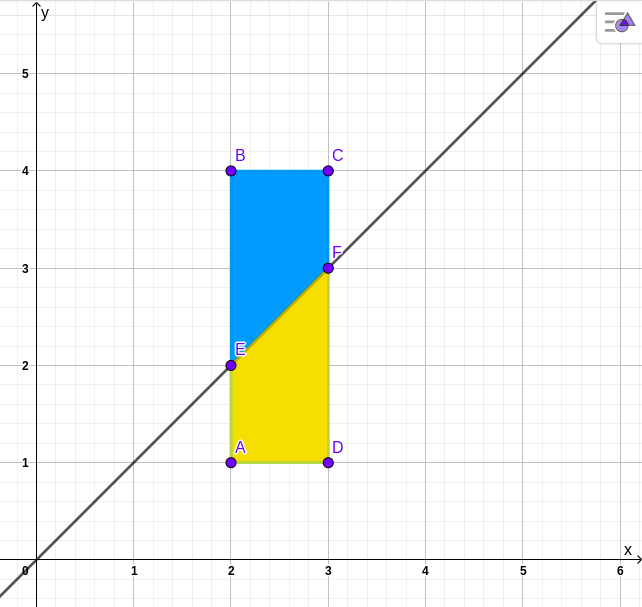
\includegraphics[width=\columnwidth]{solutions/in/2021/figures/figure.png}
\caption{Probability Distribution of (X, Y)}
\label{fig:Nuruhuhuhuhuhuhu}
\end{figure}

In figure \ref{fig:Nuruhuhuhuhuhuhu}, rectangle ABCD represents sample space of (X, Y). $Y \le X$ for any point (X, Y) if and only if the point lies on or below line EF. Therefore 
\begin{align}
    \pr{Y \le X} = \cfrac{Area\; of\; AEFD}{Area\; of\; ABCD}\\
                 = \cfrac{1}{2}    
\end{align}

Alternately, we have PDF and CDF of X and Y given by 
\begin{align}
    f_X(x) = 
    \begin{cases}
    1 & 2\le x\le 3\\
    0 & otherwise
    \end{cases}
\end{align}
\begin{align}
    F_X(x) = 
    \begin{cases}
    0   & x < 2\\
    x-2 & 2\le x\le 3\\
    1   & x > 3
    \end{cases}
\end{align}
\begin{align}
    f_Y(x) = 
    \begin{cases}
    1 & 1\le x\le 4\\
    0 & otherwise
    \end{cases}
\end{align}
\begin{align}
    F_Y(x) = 
    \begin{cases}
    0   & x < 1\\
    \cfrac{x-1}{3} & 1\le x\le 4\\
    1   & x > 4
    \end{cases}
\end{align}
Thus 
\begin{align}
    \pr{Y\le X} &= \int_{-\infty}^{\infty} F_Y(x)f_X(x)dx\\
                &= \int_2^3 \cfrac{x-1}{3}dx\\
                &= \cfrac{1}{2}
\end{align}



%
\item What is the chance that a leap year,selected at random,will contain 53 Saturdays? \\
\begin{enumerate}
    \item  $\frac{2}{7}$ 
    \item  $\frac{3}{7}$ 
    \item  $\frac{1}{7}$ 
    \item  $\frac{5}{7}$ 
\end{enumerate}
%
\solution

Let X be a random variable \\
 We Define, X $\in$ {{0,1}} \\
 \begin{table}[h]
\begin{tabular}{|l|l|}
\hline
P(X = 0) & denotes for 52 Saturday  \\ \hline
P(X = 1) & denotes for 53 Saturdays \\ \hline
\end{tabular}
\caption{$\pr{X = x}$}
\end{table}
\begin{equation}
\label{ee:2013-611}
    \implies \text{Remaining Days} = 366 - 364 = 2
\end{equation}
\begin{equation}
\label{ee:2013-612}
\implies\pr{X = 1} = \frac{2}{7}
\end{equation}
 $\therefore$ The correct answer is \textbf{Option A}
%
\item Let $X$ be the Poisson random variable with parameter $\lambda$ = 1. Then, the probability 
$\pr{2 \leq X \leq 4}$ equals ............
%
\\
\solution

Let 
\begin{align}
	X\in \{0,1,2,3,4,5...\}
\end{align}
We know that, for a poisson random variable $X$ with a given parameter $\lambda$, probability of $X=k$ is:
\begin{align} \label{eq_0}
	\pr{X=k}=\left(\frac{\lambda^k e^{-\lambda}}{k!}\right)	
\end{align}
CDF is:
\begin{align}
    F(X=k)=\sum_{x=0}^{k}\left(\frac{\lambda^x e^{-\lambda}}{x!}\right)
\end{align}
   
% The graph of CDF is shown below
% \includegraphics[width=\linewidth]{cdf.png}
And also,
\begin{align}
    \Pr\brak{x < X \le y} = F\brak{y} - F\brak{x}\label{eq_1}
\end{align}
Now by using \eqref{eq_1},
\begin{align}
    \pr{2 \leq X \leq 4} 
    & = \pr{1 < X \leq 4}\\
    & = F(4)-F(1)\\
    & = \frac{65}{24e}-\frac{2}{e}\\
    & = \frac{17}{24e}
\end{align}
\begin{figure}[ht]
    \centering
    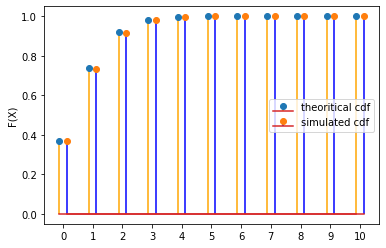
\includegraphics[width=\columnwidth]{solutions/xe/2019/simulated_theoritical.png}
    \caption{Theoretical CDF vs Simulated CDF}
    \label{Figure_0}
\end{figure}
%
\item Let the probability density function of random variable,$X$,be given as:\\
\\$f_x(x)$ = $\frac{3}{2}$$e^{-3x}$${u(x)}$ + $a$$e^{4x}$${u(-x)}$\\
\\where u(x) is the unit step function.Then the value of a and Prob\{$X\leq0$\}, respectively,are:\\
\\(A) 2,$\frac{1}{2}$\\
\\(B) 4,$\frac{1}{2}$\\
\\(C) 2,$\frac{1}{4}$\\
\\(D) 4,$\frac{1}{4}$\\
\solution
We know that,
\begin{align}
\int_{-\infty}^{\infty}{f_x(x)}\,dx = 1.\\
\int_{-\infty}^{0}{f_x(x)}\,dx +\int_{0}^{\infty}{f_x(x)}\,dx = 1\label{ee2016-33:eq_(1)}\\
\int_{-\infty}^{0}{ae^{4x}}\,dx +\int_{0}^{\infty}{\frac{3}{2}e^{-3x}}\,dx = 1\label{ee2016-33:eq_(2)}
\end{align}
The expression \eqref{ee2016-33:eq_(2)} was written from \eqref{ee2016-33:eq_(1)} since,
\begin{align*}
  u(x) = 
  \begin{cases}
  1, & \text{for } x \geq 0\\
  0, & \text{otherwise } 
  \end{cases}
\end{align*}

Simplifying \eqref{ee2016-33:eq_(2)} we have:
\begin{align}
\int_{-\infty}^{0}{ae^{4x}}\,dx +\int_{0}^{\infty}{\frac{3}{2}e^{-3x}}\,dx = 1\nonumber\\
\implies a\left[\frac{e^{4x}}{4}\right]_{-\infty}^{0} +    \frac{3}{2}\left[\frac{e^{-3x}}{-3}\right]_0^{\infty} = 1\\
\implies a\left[\frac{1}{4}-0\right] - \frac{1}{2}\left[0-1\right] = 1\\
\implies \frac{a}{4} + \frac{1}{2} =1 \implies a = 2
\end{align}
Therefore,
\begin{align}
 f_x(x) = 
  \begin{cases}
  \frac{3}{2}e^{-3x}, & \text{for } x \geq 0\\
  2e^{4x}, & \text{for } x < 0
  \end{cases}
\end{align}

The plot for PDF of $X$ can be observed at figure \ref{ee2016-33:fig:The PDF of X}
\begin{figure}[!ht]
       \centering
    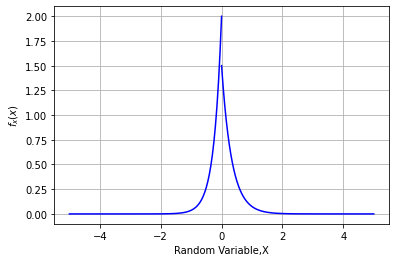
\includegraphics[width=.9\columnwidth] {solutions/ee/2016/33/Assignment_2_Fig_2.png}
    \caption{The PDF of X}
    \label{ee2016-33:fig:The PDF of X}
\end{figure}

The CDF of X is defined as follows:
\begin{align}
    F_X(x)= \pr{X\leq x}
\end{align}
Now for $x<0$,
\begin{align}
\pr{X\leq x} &= \int_{-\infty}^{x}{f_x(x)}\,dx\\
&= \int_{-\infty}^{x}{2e^{4x}}\,dx\\
&= 2\left[\frac{e^{4x}}{4}\right]_{-\infty}^{x}\\
&= 2\left[\frac{e^{4x}}{4}-0\right]\\
&= \frac{e^{4x}}{2}
\end{align}
Similarly for $x\geq0$,
\begin{align}
\pr{X\leq x} &= \int_{-\infty}^{x}{f_x(x)}\,dx\\
&= \int_{-\infty}^{0}{2e^{4x}}\,dx +\int_{0}^{x}{\frac{3}{2}e^{-3x}}\,dx\\
&= 2\left[\frac{e^{4x}}{4}\right]_{-\infty}^{0}+\left[\frac{-e^{-3x}}{2}\right]_{0}^{x}\\
&= 2\left[\frac{1}{4}-0\right]-\frac{1}{2}\left[e^{-3x}-1\right]\\
&= 1-\frac{e^{-3x}}{2}
\end{align}

The CDF of X is as below:
\begin{align}
 F_X(x) = 
  \begin{cases}
  1-\frac{e^{-3x}}{2}, & \text{for } x \geq 0\\
  \frac{e^{4x}}{2}, & \text{for } x < 0
  \end{cases}
\end{align}

The plot for CDF of $X$ can be observed at figure \ref{ee2016-33:fig:The PDF of X}.
\begin{figure}[!ht]
       \centering
    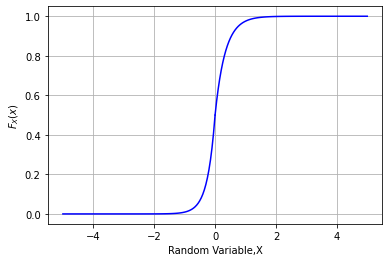
\includegraphics[width=.9\columnwidth] {solutions/ee/2016/33/Assignment_2_Fig_1.png}
    \caption{The CDF of X}
    \label{ee2016-33:fig:The CDF of X}
\end{figure}

\begin{align}
\therefore
\pr{X\leq0} = F_X(0)=\frac{1}{2}
\end{align}



%
\item  Suppose $p$ is the number of cars per minute passing through a certain road junction between $5$ $PM$ and $6$ $PM,$ and $p$ has a Poisson distribution with mean $3$. What is the probability of observing fewer than $3$ cars during any given minute in this interval$?$
\begin{enumerate}
    \item $8/(2e^3)$
    \item $9/(2e^3)$
    \item $17/(2e^3)$
    \item $26/(2e^3)$
\end{enumerate}
\solution

Probability of Poison Distribution is,
\begin{align}
    \pr{X=p}=\frac{e^{-\mu}\mu^p}{p!}
\end{align}
Here, $p$ refers to no. of cars per minute,
$p \in \{0,1,2,\dots,\infty\}$
Mean of poison distribution,
\begin{align}
    \mu=3
\end{align}
\begin{align}
    \pr{X=p}=\frac{e^{-3}3^p}{p!}
\end{align}
\begin{table}[h!]
\centering
\caption{Table of probability of no. of cars passing per minute}
\resizebox{\columnwidth}{!}{
  \begin{tabular}{||c|c|c|c|c|c||}
    \hline
    $p$ & $0$ & $1$ & $2$ & $3$ & \dots\\
    \hline
    \hline
    $\pr{X=p}$ & $1/e^3$ & $3/e^3$ & $9/(2e^3)$ & $9/(2e^3)$ & \dots\\
    \hline
  \end{tabular}
  \label{Table1}
}
\end{table}
by Boolean logic,
\begin{align}
    \pr{X<3}=\pr{X=0}+\pr{X=1}+\pr{X=2}
\end{align}
\begin{align}
    \pr{X<3}=\frac{17}{2e^3}
\end{align}
Option $(C)$ is correct
%
\item An automobile plant contracted to buy shock absorbers from two suppliers $X$ and $Y . X$ supplies $60 \%$ and $Y$ supplies $40 \%$ of the shock absorbers. All shock absorbers are subjected to a quality test. The ones that pass the quality test are considered reliable. Of X's shock absorbers, $96 \%$ are reliable. Of Y's shock absorbers, $72 \%$ are reliable.
The probability that a randomly chosen shock absorber, which is found to be reliable, is made by $Y$ is
\begin{enumerate}
\item  0.288
\item 0.334
\item  0.667
\item 0.720
\end{enumerate}
%
\solution
%
\begin{figure}[htb!]
\begin{center}
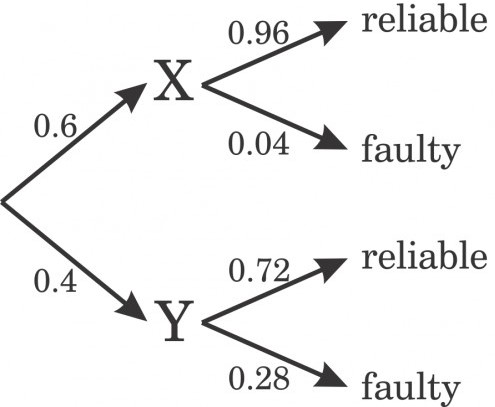
\includegraphics[width=0.5\textwidth]{solutions/cs/2012/63/Figures/A_4_1.png}
\end{center}
\end{figure}
Let Consider, Bernoulli random variables say $X,Y$ and $R$.
\begin{table}[h]
\resizebox{\columnwidth}{!}{
\begin{tabular}{|l|l|l|}
\hline
 & Refer to probability that product & Result \\ \hline
$Pr(X=1)$ & from supplier $X$ & $0.6$ \\ \hline
$Pr(Y=1)$ & from supplier $X$ & $0.4$ \\ \hline
$Pr(R=1)$ & is reliable &  \\ \hline
$Pr(R=0)$ & is faulty &  \\ \hline
$Pr(R=1/X=1)$ & from supplier $X$ is reliable & $0.96$ \\ \hline
$Pr(R=1/Y=1)$ & from supplier $Y$ is reliable & $0.72$ \\ \hline
\end{tabular}}
\caption{probability of random variables.}
\label{tab:my-table}
\end{table}
Required probability is $Pr(Y=1|R=1)$.So,
\begin{align}
&Pr(Y=1|R=1)=\frac{Pr(Y=1,R=1)}{Pr(R=1)}\\
&=\frac{Pr(Y=1)Pr(R=1/Y=1)}{Pr(X=1)Pr(R=1/X=1)+Pr(Y=1)P(R=1/Y=1)}\\
&=\frac{(0.4)(0.72)}{(0.6)(0.96)+(0.4)(0.72)}=0.334
\end{align}
%
\item The probability of a resistor being defective is 0.02. There are 50 such resistors in a circuit. The probability of two or more defective resistors in the circuit (round off to two decimal places) is ---
%
\solution
Consider, Probability of a defective resistor 
$= P   = 0.02 = \dfrac{1}{50}$. \\
Total number of resistors = n = 50. \\
Let X be number of defective resistors. \\
By Binomial distribution, \\
\begin{align}
Pr(X = k) = \binom{n}{k}\brak{P}^k\brak{1 - P}^{n-k} 
\end{align}
\begin{align}
Pr(X = 0) &= \binom{50}{0}\brak{\dfrac{1}{50}}^0\brak{1 - \dfrac{1}{50}}^{50-0} 
\end{align}
\begin{align}
\implies Pr(X = 0) &= \brak{\dfrac{49}{50}}^{50} 
\end{align}
\begin{align}
Pr(X = 1) &= \binom{50}{1}\brak{\dfrac{1}{50}}^1\brak{1 - \dfrac{1}{50}}^{50-1} 
\end{align}
\begin{align}
\implies Pr(X = 1) &= \brak{\dfrac{49}{50}}^{49}
\end{align}
\begin{align*}
\Pr{(X \ge 2)} &= 1 - \Pr{(X < 2)} \\
\Pr{(X \ge 2)} &= 1 - \brak{\Pr{(X = 0)} + \Pr{(X = 1)}} \\
\Pr{(X \ge 2)} &= 0.2642 
\end{align*}
%
\item A person who speaks truth $3$ out of $4$ times,throws a fair dice with six faces and informs the outcome is $5$.The probability that the outcome is really $5$ is
\\
\solution
Let $X \in \{0,1\}$ represent the random variable,where $0$ represents person speaking false,$1$ represents person speaking truth.\\
Let $Y \in \{1,2,3,4,5,6\}$  represent random variable,where $1,2,3,4,5,6$ represents person informs outcome of dice is $1,2,3,4,5,6$,respectively.\\
\begin{table}[h!]
\resizebox{\columnwidth}{!}
{ 
\begin{tabular}{|c|c|c|}
\hline
Event & definition & value\\
\hline
$ \pr{X=1} $ & Probability of person  & $\frac{3}{4}$\\
&speaking truth & \\
\hline
$ \pr{X=0} $ & Probability of person & $\frac{1}{4}$ \\
& speaking false & \\
\hline
$\pr{Y=5|X=1}$ & Probability of person  & \\
&  informing outcome is $5$ & $\frac{1}{6}$  \\
& if person speaks truth & \\
\hline
$\pr{Y=5|X=0}$ & Probability of person & \\
& informing outcome is $5$ &  $\frac{5}{6}$ \\
& if person speaks false & \\ 
\hline
\end{tabular}
}
\caption{Table 1} 
\label{xe2021-9:tab:1}
\end{table}
From Baye's theorem
\begin{align}
\pr{Y=5}&=\pr{Y=5|X=1} \times \pr{X=1} \notag \\
 & +\pr{Y=5|X=0} \times \pr{X=0}  \label{xe2021-9:1}
 \end{align}
Substiting values from table \eqref{xe2021-9:tab:1} in \eqref{xe2021-9:1}
\begin{align}
\pr{Y=5} &=\frac{8}{24} \label{xe2021-9:2} \\
\pr{(X=1)(Y=5)}&= \pr{Y=5|X=1} \notag \\
& \times \pr{X=1} \\ 
&= \frac{3}{24}  \label{xe2021-9:3}
\end{align}
We need to find $\pr{X=1|Y=5}$ \\
\begin{align}
\pr{X=1|Y=5} &= \frac{\pr{(X=1 ) (Y=5)}}{\pr{Y=5}} \\
&=\frac{3}{8}
\end{align}
%
\item  The probabilities that a student passes in Mathematics, Physics and Chemistry are m,p, and
c respectively. Of these subjects, the student has 75\% chance of passing in at least one, a
50\% chance of passing in at least two and a 40\% chance of passing in exactly two.
Following relations are drawn in m, p, c:
    \begin{enumerate}[label=(\Roman*)]
        \item p + m + c = 27/20
        \item p + m + c = 13/20
        \item (p)$\times$ (m) $\times$ (c) =1/10
    \end{enumerate}
    \begin{enumerate}[label=(\Alph*)]
      \item Only relation I is true
      \item Only relation II is true
      \item Relations II and III are true
      \item Relations I and III are true
    \end{enumerate}
%
\solution

Let M,P,C be the events representing student passes in Mathematics,Physics,Chemistry respectively.
\begin{align}
    \pr{M}&=m\\
    \pr{P}&=p\\
    \pr{C}&=c
\end{align}
The given information can be represented as
\begin{align}
    \pr{M+P+C}=75\%=\dfrac{3}{4}\label{atleast_1}\\
    \pr{MP+PC+CA}=50\%=\dfrac{1}{2}\label{atleast_2}\\
    \pr{MP+PC+CA-3MPC}=40\%=\dfrac{2}{5} \label{only_2}
\end{align}
\eqref{atleast_2} and \eqref{only_2} can also be written as
\begin{align}
    \pr{MP}+\pr{PC}+\pr{CM}&\nonumber\\-2\pr{MPC}&=\dfrac{1}{2}\\
    \pr{MP}+\pr{PC}+\pr{CM}&\nonumber\\-3\pr{MPC}&=\dfrac{2}{5}
\end{align}
Subtracting and solving the above two equations we get,
\begin{align}
    \pr{MPC}&=\dfrac{1}{10}\\
    \pr{MP}+\pr{PC}+\pr{CM}&=\dfrac{7}{10}
\end{align}
Using inclusion-exclusion principle, We can express \eqref{atleast_1} as
\begin{align}
\pr{M}+\pr{P}+\pr{C}&\nonumber\\
-[\pr{MP}+\pr{PC}+\pr{CM}]&\nonumber\\
      +\pr{MPC}&=\dfrac{3}{4}\\
    p+m+c-\dfrac{7}{10}+\dfrac{1}{10}&=\dfrac{3}{4}\\
    p+m+c&=\dfrac{27}{10}
\end{align}
There is no constant answer for the product of p,m,c which is shown in simulation.\\\\
\centering $\therefore$ Only relation I is true.
%
\item 
\solution


Let $F_X(t)$ denote the Cumulative Distribution Function for random variable $X$.\\
\begin{align}
F_X(t) &= \int_{-\infty}^{t} f(t) \,dt
\\[\parskip]
&= \int_{-\infty}^{0} 0 \,dt + \int_{0}^{t} e^{-t} \,dt
\\[\parskip]
&= -e^{-t}\Big|_{0}^t
\\[\parskip]
&= 1-e^{-t}
\end{align}
\begin{align}
P(X\leq b|X\geq a) &= \dfrac{P((X\leq b),(X\geq a))}{P(X\geq a)}
\\[\parskip]
&= \dfrac{P(a\leq X \leq b)}{P(X\geq a)}
\\[\parskip]
&=\dfrac{F_X(b)-F_X(a)}{\displaystyle\lim_{k\to\infty} F_X(k)-F_X(a)}
\\[\parskip]
&=\dfrac{e^{-a}-e^{-b}}{e^{-a}}
\\[\parskip]
&=1-e^{-(b-a)}
\end{align}
Therefore the required probability depends on $b-a$\\


%
\item Let $X$ and $Y$ denote the sets consisting 2 and 20 distinct elements respectively and $F$ denote the set of all possible functions defined from $X$ and $Y$. Let $f$ be randomly chosen from $F$. The probability of f being one to one is :
\\
\solution
We know, every $x \in X$ can be mapped to one of 20 elements in $Y$.
\begin{align}
    n(F) = 20 \times 20 = 400
\end{align}

For one to one functions,  the first element in $X$ has 20 elements it can be mapped to, and second element in $X$ has only 19 elements.(to avoid repetition).
\begin{align}
    n(f) = 20 \times 19 = 380
\end{align}
Required probability:
\begin{align}
    \frac{n(f)}{n(F)} = \frac{380}{400} = \frac{19}{20}
\end{align}
%
\item Let $S$ be a sample space and two mutually exclusive events $A$ and $B$ be such that $A + B = S$. If $P(\cdot)$ denotes the probability of the event, the maximum value of $P(A)P(B)$ is
\\
\solution
\begin{align}
\Pr(A+B) &= 1\\
\Pr(A) + \Pr(B) &= 1 \\
\Pr(A)\Pr(B) &= \Pr(A) (1 - \Pr(A))\\
&= \Pr(A) - (\Pr(A))^2\\
&= \dfrac{1}{4} - \left( \Pr(A) - \dfrac{1}{2} \right)^2 \\
&\leq \dfrac{1}{4}\\
\Pr(A) = \Pr(B) = \dfrac{1}{2} &\Rightarrow \Pr(A)\Pr(B) = \dfrac{1}{4}\\ \therefore \text{max}(\Pr(A)\Pr(B)) &= \dfrac{1}{4}
\end{align}
%
% \item Let $X$ be the Poisson random variable with parameter $\lambda$ = 1. Then, the probability 
% $\pr{2 \leq X \leq 4}$ equals ............
% %
% \solution
% 
Let 
\begin{align}
	X\in \{0,1,2,3,4,5...\}
\end{align}
We know that, for a poisson random variable $X$ with a given parameter $\lambda$, probability of $X=k$ is:
\begin{align} \label{eq_0}
	\pr{X=k}=\left(\frac{\lambda^k e^{-\lambda}}{k!}\right)	
\end{align}
CDF is:
\begin{align}
    F(X=k)=\sum_{x=0}^{k}\left(\frac{\lambda^x e^{-\lambda}}{x!}\right)
\end{align}
   
% The graph of CDF is shown below
% \includegraphics[width=\linewidth]{cdf.png}
And also,
\begin{align}
    \Pr\brak{x < X \le y} = F\brak{y} - F\brak{x}\label{eq_1}
\end{align}
Now by using \eqref{eq_1},
\begin{align}
    \pr{2 \leq X \leq 4} 
    & = \pr{1 < X \leq 4}\\
    & = F(4)-F(1)\\
    & = \frac{65}{24e}-\frac{2}{e}\\
    & = \frac{17}{24e}
\end{align}
\begin{figure}[ht]
    \centering
    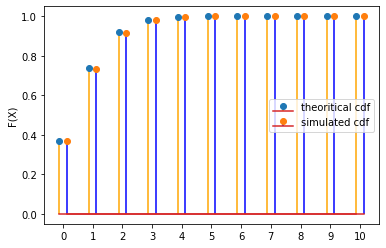
\includegraphics[width=\columnwidth]{solutions/xe/2019/simulated_theoritical.png}
    \caption{Theoretical CDF vs Simulated CDF}
    \label{Figure_0}
\end{figure}
%
\item Given Set A = \{2,3,4,5\} and Set B = \{11,12,13,14,15\}, two numbers are randomly selected, one from each set. What is probability that the sum of the two numbers equals 16?
\\
%
\solution

Let $X_1\in\,$\cbrak{2,3,4,5} and $X_2\in\,$\cbrak{11,12,13,14,15} be the random variables such that $X_1$ represents the number chosen from set A and $X_2$ the number chosen from set B.\\
Then, the probability mass functions are 
\begin{align}
    p_{X_1}(n) = \pr{X_1 = n} = 
    \begin{cases}
    \frac{1}{4} & 2 \leq n \leq 5\\
    0 & otherwise
\end{cases}\label{ee2015-2:1}
\end{align}
\begin{align}
    p_{X_2}(n) = \pr{X_2 = n} = 
    \begin{cases}
    \frac{1}{5} & 11 \leq n \leq 15\\
    0 & otherwise
\end{cases}\label{ee2015-2:2}
\end{align}
Let X be the random variable denoting the sum (X=$X_1$+$X_2$). Then, X can take the values \cbrak{13,14,15,16,17,18,19,20}.
\begin{align}
     p_X(n)&=\pr{X_1+X_2=n}\\
     &=\pr{X_1=n-X_2}\\
     &=\Sigma_{k}{\pr{X_1=n-k|X_2=k}p_{X_2}(k)}\label{ee2015-2:3}
\end{align}
 As $X_1,X_2$ are independent,
\begin{align}
    \pr{X_1=n-k|X_2=k}=\pr{X_1=n-k}\label{ee2015-2:4}
\end{align}
from \eqref{ee2015-2:3} and \eqref{ee2015-2:4}
\begin{align}
    p_X(n) = \Sigma_{k} p_{X_1}(n-k)p_{X_2}(n)
    &= p_{X_1}(n)*p_{X_2}(n)\label{ee2015-2:5}
\end{align}
where * denotes the convolution operator.\\
As,
\begin{align}
    p_X(n) &= \Sigma_{k} p_{X_1}(n-k)p_{X_2}(k)\\
    &= \frac{1}{5} \sum_{k=11}^{15}p_{X_1}(n-k)\\
    &= \frac{1}{5} \sum_{k=n-15}^{n-11} p_{X_1}(k)
\end{align}
Since $p_{X_1}(k)=0$ for $k<2 , k>5$\\
Therefore, we get 
\begin{align}
    p_x(n) = 
    \begin{cases}
    0 & n \leq 12\\
    \frac{1}{5} \sum_{k=2}^{n-11}p_{X_1}(k) & 2 \leq n-11 \leq 5\\
    \frac{1}{5} \sum_{k=n-15}^{5}p_{X_1}(k) & 2 \leq n-15 \leq 5\\
    0 & n>20
    \end{cases}
\end{align}
Therefore, from \eqref{ee2015-2:1} we get
\begin{figure}[!hbt]
    \centering
    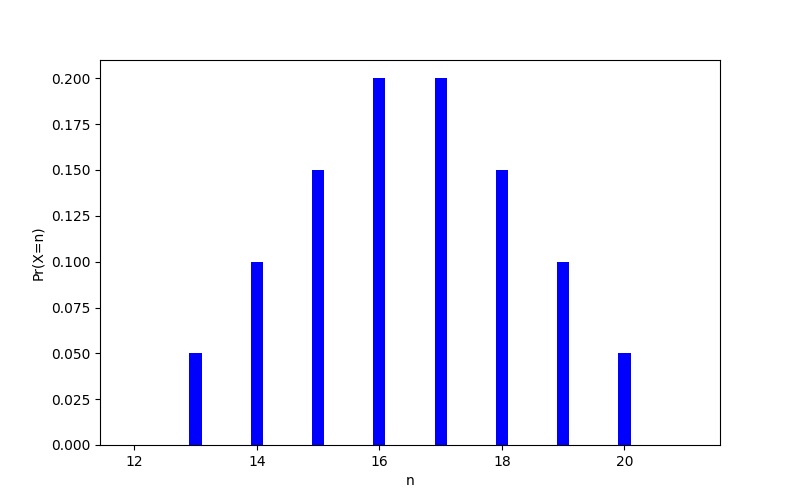
\includegraphics[width=\columnwidth]{solutions/ee/2015/2/Figure_1.png}
    \caption{Probability mass function of X}
    \label{ee2015-2:Figure_1}
\end{figure}
\begin{align}
    p_x(n) = 
    \begin{cases}
    0 & n \leq 12\\
    \frac{n-12}{20}  & 13 \leq n \leq 16\\
    \frac{21-n}{20}  & 17 \leq n \leq 20\\
    0 & n>20
    \end{cases}\label{ee2015-2:6}
\end{align}
Required probability is the probability of the sum of numbers selected from the sets, one from each set to be 16.\\
Therefore from \eqref{ee2015-2:6},
\begin{align}
    p_X(16) &= \left(\frac{16-12}{20}\right)\\
    \implies p_X(16) &= \frac{4}{20}\\
    \implies\pr{X_1+X_2=16} &= \frac{1}{5} \\
    \therefore \pr{X_1+X_2=16}  &= 0.2
\end{align}

%
\item For each element in a set of size 2n, an unbiased coin is tossed. The 2n coin tosses are independent. An element is chosen if the corresponding coin toss were head. The probability that exactly n elements are chosen is:\\
\begin{enumerate}
    \item $\frac{\comb{2n}{n}}{4^{n}}$ \hspace{1cm}\\
    \item $\frac{\comb{2n}{n}}{2^{n}}$ \hspace{1cm}\\
    \item $\frac{1}{\comb{2n}{n}}$ \hspace{1cm}\\
    \item $\frac{1}{2}$
\end{enumerate}
%
\solution

The number of elements chosen is equal to the number of heads obtained by 2n coin tosses.
Let X be a random variable with value of X equal to the number of heads obtained.\\
Probability of getting a head, $p=\frac{1}{2}$\\
Probability of getting a tail, $q=\frac{1}{2}$\\
Probability that n elements are chosen out of 2n elements is \pr{X=n}\\
From binomial distribution we know that,
\begin{align}
\pr{X=r}&=\comb{2n}{r}p^{r}q^{2n-r}\\
\pr{X=n}&=\comb{2n}{n} \times \brak{\frac{1}{2}}^{n}  \times \brak{\frac{1}{2}}^{n}\\
        &=\frac{\comb{2n}{n}}{4^{n}}
\end{align}
Hence option (A) is correct.

%
\item Players A and B take turns to throw a fair dice with six faces. If A is the first player to throw, then the probability of B being the first one to get a six is --- ( round of to two decimal places). \\
\solution

Let the random variable X represent which player gets six first. That is $X=0 $ when A gets a six first and $X=1 $ when B gets six first. \\
Let another random variable Y represent getting a six on the dice. $Y=1 $ for six and $Y=0 $ for any other number. \\
Let N be the number of turns until we get a six.
\begin{align}
    \Pr\brak{Y=0} = \frac{5}{6} \\
    \Pr\brak{Y=1} = \frac{1}{6}
\end{align}
The event success is when B gets a six for first time and failure is when neither A nor B gets six. Let p denote probability of success 
\begin{align}
    p &= \Pr\brak{Y=1}  \\
    \Pr\brak{Y=0} &= 1- p \\
    p &= \frac{1}{6}
\end{align}
To get $X=1 $ in $N$ turns we have to get $N-1$ failures for B and $ N$ failures for A and finally one success for B. 
Therefore the geometric distribution is,
\begin{align}
    f(N) &= \brak{1-p}^{n-1} \times p \times  \brak{1-p}^{n} \\
    &  = \brak{1-p}^{2n-1} \times p \\
    & = \brak{ \frac{5}{6}}^{2n-1} \times \frac{1}{6}
\end{align}
The result has been summarized in table \ref{tab:table geometric distribution}. \\
\begin{table}[hbt!]
\centering
\begin{tabular}{|c|c|}
\hline
\textbf{No. of turns} & \textbf{Probability} \\ \hline
1                     & $5^1/6^2  $            \\ \hline
2                     & $5^3/6^4 $             \\ \hline
$\vdots  $              & $\vdots $              \\
n                     & $5^{2n-1}/6^{2n} $         \\ \hline
$\vdots $               & $\vdots $              \\ \hline
\end{tabular}
\caption{Summary of turns}
\label{tab:table geometric distribution}
\end{table}
Thus the total probability is sum of these individual probabilities i.e.
\begin{align}
    \Pr\brak{X=1} &= \sum_{N=1}^{\infty} f(N) \\
    &= \frac{5}{6^2} + \frac{5^3}{6^4} + \hdots + \frac{5^{2n-1}}{6^{2n}} +\hdots  \\
    &= \frac{5}{6^2} \times \brak{1 + \frac{5^2}{6^2} + \frac{5^4}{6^4} + \hdots } 
\end{align}
By Using sum of infinite GP we have, 
\begin{align}
     \Pr\brak{X=1} &= \frac{5}{6^2} \times \brak{\frac{1}{1 - \frac{25}{36}}}  \\
       &= \frac{5}{36} \times \frac{36}{11} \\
       &= \frac{5}{11} = 0.45
\end{align}
%
\item The probability that a number selected at random between 100 and 999 (both inclusive) will not contain digit 7 is.
\solution

Let's assume a random 3-digit number be $xyz$.\\
Where $x,y,z$ are 3 random single-digit integers such that
\begin{align}
x\in \{1,2,3,4,5,6,7,8,9\}\\
y\in \{0,1,2,3,4,5,6,7,8,9\}\\
z\in \{0,1,2,3,4,5,6,7,8,9\}
\end{align}
\begin{enumerate}
\item
Probability of selecting $x$ without including 7
\begin{align}
    \Pr{(x\neq 7)}&=\frac{8}{9}
\end{align}
\item
Probability of selecting $y$ without including 7
\begin{align}
    \Pr{(y\neq 7)}&=\frac{9}{10}
\end{align}
\item
Probability of selecting $z$ without including 7
\begin{align}
    \Pr{(z\neq 7)}&=\frac{9}{10}
\end{align}
\end{enumerate}
So,the total probability of a random 3-digit number $xyz$ will not contain 7\\
\begin{align}
    &=\Pr{(x\neq 7)}\times\Pr{(y\neq 7)}\times\Pr{(z\neq 7)}\\
    &=\frac{8}{9}\times\frac{9}{10}\times\frac{9}{10}\\
    &=\frac{18}{25}
\end{align}
The probability of a number selected at random between 100 and 999 (both inclusive) will not contain digit 7 is $\frac{18}{25}$
%
\item A class of twelve children has two more boys than girls. A group of three children are randomly picked from this class to accompany the teacher on the field trip. What is the probability that the group accompanying the teacher contains more girls than boys.\\
\begin{enumerate}[label=(\alph*)]
\item $0$\\
\item $\frac{325}{864}$ \\
\item$\frac{525}{864}$\\
\item$\frac{5}{12}$
\end{enumerate}
\solution


Let $X \in \{0,3\}$ be a discrete random variable which denotes the number of girls in the group of 3.\\ 
Since, there are two more boys than girls:\\
\begin{align}
    \text{Total number of boys} (B) = 7  \notag \\
    \text{Total number of girls} (G) = 5  \notag\\
    \pr{X=c}=\frac{\comb{5}{c}\times \comb{7}{3-k}}{\comb{12}{3}} \label{ee2018-8:1.0.1}
\end{align}


For number of girls more than boys required probability = $ \pr{2\le X \le 3}$ and hence, following cases are possible. 
\begin{enumerate}
    \item X=3
    \begin{align}
        \pr{X=3} = \frac{\comb{5}{3}}{\comb{12}{3}}, \text{using \eqref{ee2018-8:1.0.1}} \notag
    \end{align}
    \item X=2
    \begin{align}
        \pr{X=2} = \frac{\comb{5}{2}\times\comb{7}{1}}{\comb{12}{3}}, \text{using \eqref{ee2018-8:1.0.1}} \notag
    \end{align}
\end{enumerate}
\begin{align}
   \text {So, required probability }=  \frac{\comb{5}{2}\times\comb{7}{1}}{\comb{12}{3}} + \frac{\comb{5}{3}}{\comb{12}{3}} = \frac{4}{11} \notag
\end{align}


%
\item Suppose that a shop has an equal number of LED bulbs of two different types. The probability of an LED bulb lasting more than 100 hours given that it is of Type 1 is 0.7, and given that it is of Type 2 is 0.4. The probability that an LED bulb chosen uniformly at random lasts more than 100 hours is
\\
\solution 

Let the random variable $X\in\{1,2\}$ represent the type of the chosen bulb. $X=1$ denotes a Type 1 bulb, while $X=2$ denotes a Type 2 bulb. Given,
\begin{align}
\tag{5.1}
    n(X=1)=n(X=2)\\
\tag{5.2}\Rightarrow p_{X}(1)=p_{X}(2)=\dfrac{1}{2}
\end{align}
Let the random variable $Y\in\{0,1\}$ represent if a bulb lasts more than 100 hours. $Y=1$ denotes that it lasts, while $Y=0$ denotes that it doesn't. Given, 
\begin{align}
\tag{5.3}
    p_{Y|X}(1|1)=0.7\\
\tag{5.4}
    p_{Y|X}(1|2)=0.4
\end{align}
To find : $p_{Y}(1)$
\begin{align}
\tag{5.5}
p_{Y}(1)&=p_{Y|X}(1|1)p_{X}(1)+p_{Y|X}(1|2)p_{X}(2)\\
\tag{5.6}
&p_{Y}(1)=(0.7)(0.5)+(0.4)(0.5)\\
\tag{5.7}
&\therefore p_{Y}(1)=0.55
\end{align}
%
\item Suppose $X_i$ for $i = 1, 2, 3$ are independent
and identically distributed random variables
whose probability mass functions are
$\pr{X_i = 0} = \pr{X_i = 1} = \frac{1}{2}$ for $i = 1, 2, 3$.
Define another random variable $Y = X_1 X_2 \oplus X_3$, where $\oplus$ denotes XOR. Then $\pr{Y = 0|X_3 = 0} =$
\\
\solution 

For
\begin{align}
    \because Y = (X_1X_2) \oplus X_3 &= 0\\
    \implies X_1X_2 &= X_3 \label{cs2015-37:all_equal}
\end{align}
\begin{align}
    \pr{Y=0|X_3=0} &= \dfrac{\pr{Y=0,X_3=0}}{\pr{X_3=0}} \label{cs2015-37:eq:0.0.1}\\
    &=\dfrac{\pr{X_1X_2 = X_3, X_3 = 0}}{\pr{X_3=0}}\\
    \pr{X_3 = 0} &= \frac{1}{2} \label{cs2015-37:eq:0.0.2}
\end{align}
if $X_3 = 0$, from \eqref{cs2015-37:all_equal}
\begin{align}
    X_1X_2 &= 0
\end{align}
%The number of possibilities for $X_1X_2=0$
%\begin{align}
%    (X_1,X_2) = \begin{cases}
%(0,0)\\(0,1)\\(1,0)
%\end{cases}
%\end{align}
The random variables are independent of each other:
%\begin{align}
%    \pr{X_i = a, X_j = b} &= \pr{X_i=a} \cdot \pr{X_j=b}\\
%    i \neq j,\quad i,j &\in \{1,2,3\}\\
%    a,b &\in \{0,1\}
%\end{align}
\begin{table}[h!]
    \centering
    \resizebox{\columnwidth}{!}
    {
    \begin{tabular}{|c|c|c|}
    \hline
         $\pr{X_1=0,X_2=0}$& $\pr{X_1=0}\cdot\pr{X_2=0}$&$0.25 $\\ \hline
         
         $\pr{X_1=1,X_2=0}$&$\pr{X_1=1}\cdot\pr{X_2=0}$&$0.25$ \\  \hline
         $\pr{X_1=0,X_2=1}$&$\pr{X_1=0}\cdot\pr{X_2=1}$&$0.25$\\
         \hline
    \end{tabular}
    }
    
    \caption{Probabilities }
    \label{cs2015-37:tab:my_label}
\end{table}
\begin{align}
\nonumber
\pr{X_1X_2=0} &= \pr{X_1=0,X_2=0} \\ \nonumber
    &\quad+ \pr{X_1=0,X_2=1}\\ &\quad+ \pr{X_1=1,X_2=0}\\
    &=\frac{1}{4} +\frac{1}{4} + \frac{1}{4}= \frac{3}{4} 
\end{align}
\begin{align}
    \pr{Y=0,X_3=0} &= \pr{X_1X_2=X_3=0}\\
    &= \pr{X_1X_2=0}\cdot\pr{X_3=0}\\
    &=\frac{3}{4} \cdot \frac{1}{2}\\
    &=\frac{3}{8} \label{cs2015-37:case_A}
\end{align}
Upon substituting \eqref{cs2015-37:case_A} and \eqref{cs2015-37:eq:0.0.2} in \eqref{cs2015-37:eq:0.0.1}
\begin{align}
    \pr{Y=0|X_3=0} = \dfrac{3}{4} = 0.75
\end{align}
%
\item The probability that a given positive integer lying between 1 and 100 ( both inclusive) and is NOT divisible by 2 or 3 or 5 is \dots
\\
\solution
Let $A,B,C$ are events where a positive integer between 1 and 100 ( both inclusive ) is divisible by 2, 3, 5 respectively.
\begin{align}
  \Pr(A) &= \frac{1}{2}\\
  \Pr(B) &= \frac{33}{100} \\
  \Pr(C) &= \frac{1}{5} \\
  \Pr(AB) &= \frac{16}{100} \\
  \Pr(BC) &= \frac{6}{100} \\
  \Pr(AC) &= \frac{1}{10} \\
  \Pr(ABC) &= \frac{3}{100} 
\end{align}
Required probability : $\Pr(A+B+C)^{\prime}$
\begin{multline}
\Pr(A+B+C)^{\prime}  = 1-\Pr(A+B+C) \\  
 = 1-\Pr(A)-\Pr(B)-\Pr(C)+{}\\ \Pr(AB) + \Pr(BC)+ \Pr(AC){}\\
 -\Pr(ABC) 
    = 0.26 
\end{multline}
%
\item  In an industry, the probability of an accident occurring in a given month is $\frac{1}{100}$. Let $\pr{n}$ denote the probability that there will be no accident over a period of '$n$' months. Assume that the events of individual months are independent of each other. The smallest integer value of '$n$' such that $\pr{n}\le \frac{1}{2} $ is .............(\textit{round off to the nearest integer}).\\
%
\solution
Let A be the event of an accident occurring in a given month.
So, 
\begin{align}
    \pr{A}&=\frac{1}{100}\\
    \pr{A^{\prime}}&=1-\pr{A}\\
    \pr{A^{\prime}}&=\frac{99}{100}
\end{align}
So, $\pr{n}$ can be written as:
\begin{align}
    \pr{n}=\pr{A^{\prime}\times A^{\prime}\cdots A^{\prime}}_{A^{\prime}\; n\; times}
\end{align}
Its given that events of individual months are independent of each other, so
\begin{align}
    \pr{n}&=\pr{A^{\prime}}\cdot \pr{A^{\prime}} \cdots \pr{A^{\prime}}_{A^{\prime}\; n\; times}\\
        &=(\pr{A^{\prime}})^n \label{eq_ind}
\end{align}
Given:
\begin{align}
    \pr{n}\le \frac{1}{2}
\end{align}
So, from \eqref{eq_ind},
\begin{align}
    (\pr{A^{\prime}})^n\le \frac{1}{2} \label{eq_log}
\end{align}
\begin{align}
     \implies \ln{ (\pr{A^{\prime}})^n} &\le \ln {\frac{1}{2}}\\
     \implies n\cdot \ln {\frac{99}{100}} &\le \ln {\frac{1}{2}}\\
     \implies n &\ge \frac{\ln {\frac{1}{2}}}{\ln {\frac{99}{100}}}\\
     \implies n &\ge 68.9675
\end{align}
$\therefore$ The smallest integer value of n is \textbf{69}. 
  

%
\item Let $X_1$, $X_2$, $X_3$ and $X_4$ be independent normal random variables with zero mean and unit variance. The probability that $X_4$ is the smallest among the four is..... 
\\
\solution
Required probability
\begin{align}
    &= \pr{X_4 = min(X_1, X_2, X_3, X_4)}\\
    &= \int_{-\infty}^{\infty}\pr{X_1, X_2, X_3 > x | X_4 = x}
\end{align}
Since $X_1$, $X_2$, $X_3$ and $X_4$ are independent, required probability
\begin{align}
    &= \int_{-\infty}^{\infty} (1-F_{X_1}(x))(1-F_{X_2}(x))(1-F_{X_3}(x))f_{X_4}(x)dx\\
    &= \int_{-\infty}^{\infty} (1-\Phi(x))^3\phi(x)dx
\end{align}
Substituting 
\begin{align}
    u  &= 1 - \Phi(x)\\
    du &= -\phi(x)dx
\end{align}
we get required probability
\begin{align}
    = -\int_1^0 u^3 du\label{simplifiedintegral}\\
    = \cfrac{1}{4}
\end{align}
Note that in eq. \eqref{simplifiedintegral} the  integral is from 1 to 0 because
\begin{align}
    1-\Phi(-\infty) &= 1\\
    1-\Phi(\infty)  &= 0
\end{align}
Here $\phi(x)$ and $\Phi(x)$ represent the pdf and cdf of standard normal random variable respectively.
%
\item Let X and Y be two statistically independent random variables uniformly distributed in the range (-1, 1) and (-2, 1) respectively. Let $Z = X +Y$ , then the probability that $[Z \leq -2]$ is\\
(A) 0\\
(B) $\frac{1}{6}$\\
(C) $\frac{1}{3}$\\
(D) $\frac{1}{12}$
%\\
%\solution
%\input{solutions/ec/2003/61/Assignment_4.tex}
%
\item What is the probability that a divisor of $10^{99}$ is a multiple of $10^{96}$ ?
\vspace{0.5 cm}
(A) $\dfrac{1}{625}$ \hspace{0.5 cm} (B) $\dfrac{4}{625}$ \hspace{0.5 cm} (C) $\dfrac{12}{625}$ \hspace{0.5 cm} (D) $\dfrac{16}{625}$
%
\\
\solution
Let 
\begin{align*}
& X= \{ (x,y) : 0\leq x \leq 99 ,0\leq y \leq 99 \}
\end{align*} 
be a set of random variables, $N=2^x5^y$ , 
\begin{align}
& \implies \forall (x,y) \in X, \text{ N is a divisor of } 10^{99}\\
&\implies n (X) = 100\times 100=10^4 \label{cs2010-27:eq_1}
\end{align}
Let 
\begin{align*}
&Y=\{(x,y) : (x,y)\in X , x \geq 96,y\geq 96\}\\
&N_1= 2^x5^y 
\end{align*}
\begin{align}
&\implies \forall (x,y) \in  Y ,N_1 | 10^{99} \text{ and is multiple of } 10^{96} \\
&\implies n(Y)=4\times 4=16 \label{cs2010-27:eq_2}
\end{align}
Let P denotes the probability that a divisor of $10^{99}$ is a multiple of $10^{96}$ then
$$P=\dfrac{n(Y)}{n(X)}$$
From \ref{cs2010-27:eq_1} and \ref{cs2010-27:eq_2} we can write
$$P=\dfrac{16}{10^4}=\dfrac{1}{625}$$
So the probability is $\dfrac{1}{625}$, option (\textbf{A}).
%
\item There are five bags each containing identical sets of ten distinct chocolates. One chocolate is picked from each bag.\\
The probability that atleast two chocolates are identical is?\\
\solution

Let random variable $X\in\{0,2,3,4,5\}$ denote the maximum number of identical chocolates picked in an experiment.
\begin{align}
    P\brak{X\geq2} &= 1-P\brak{X=0}\\
    &=1-\frac{10\times9\times8\times7\times6}{10^{5}}\\
    &=1-0.3024\\
    &=0.6976
\end{align}

%
\item Raju has four fair coins and one fair dice. At first Raju tosses a coin. If the coin shows head then he rolls the dice and the number that dice shows is taken as his score. If the coin shows tail then he tosses three more coins and the total number of tails shown (including the first one) is taken as his score. If Raju tells that his score is 2 then the probability that he rolled the dice is (up to two decimal places):
%
\\
\solution
Let $X_i$ denote the random variable function for the $i$th coin $i\in\{1,2,3,4\}$.\\
$X_i\in(0,1)$ where 0 represents head and 1 represents tail $i\in\{1,2,3,4\}$.
\\[5pt]
\begin{tabular}{|c|c|c|}
\hline
     &Head&Tail  \\
     \hline
     $X_i=k$&0&1\\
     \hline
\end{tabular}
\begin{equation}\label{ec29-1:coin}
\Pr(X_i=k)=\dfrac{1}{2} 
\end{equation}
$k\in\{0,1\}$ and $i\in\{1,2,3,4\}$.
\\
Let $Y$ denote the random variable function for the dice.\\
$Y\in(1,2,3,4,5,6)$ where 1 represents dice showing 1 and so on.
\\[5pt]
\begin{tabular}{|c|c|c|c|c|c|c|}
\hline
     Dice number&1&2&3&4&5&6  \\
     \hline
     $Y=k$&1&2&3&4&5&6\\
     \hline
\end{tabular}
\\
\begin{equation}\label{ec29-1:dice}
\Pr(Y=k)=\dfrac{1}{6} 
\end{equation}
$k\in\{1,2,3,4,5,6\}$.
\\[20pt]
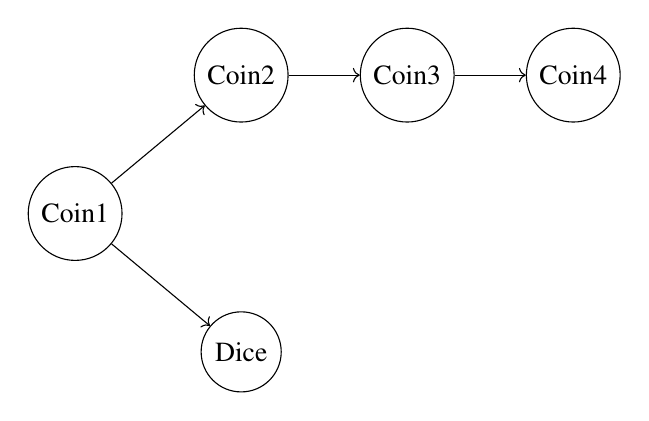
\begin{tikzpicture}
      [sibling distance=10em,level distance=6em, grow=right,
      every node/.style={shape=circle,draw,align=center},->]
      \node{Coin1}
   child
   {
    node{Dice}
   }
   child
   {
    node{Coin2}
      child
      {
        node{Coin3}
        child
      {
        node{Coin4}
      }
      }
    };
\end{tikzpicture}
Let B denote the event that out of last three coins, only one shows tail. \\
By Binomial Distribution,
\begin{align}
\Pr(B)&=\comb{3}{1}\brak{{\dfrac{1}{2}}}^3
\\[\parskip]
&=\dfrac{3}{8}
\end{align}
%
Since tossing a coin and rolling a dice are independent events,
\begin{equation}\label{ec29-1:independent theorem}
\Pr( (X_i=k),(Y=l) )= \Pr(X_i=k)\cdot \Pr(Y=l)
\end{equation}
$k\in\{0,1\}$ and $l\in\{1,2,3,4,5,6\}$.

Let A denote the event that the score is 2.

Clearly,
\begin{align}
\Pr(A)\nonumber&=\Pr(Y=2|X_1=0)\cdot \Pr(X_1=0) \\
    &+ \Pr(B|X_1=1)\cdot \Pr(X_1=1) 
\\[\parskip]
&=\Pr( (X_1=0),(Y=2) ) + \Pr( (X_1=1), B)
\\[\parskip]
&=\Pr(X_1=0)\cdot \Pr(Y=2)+ \Pr(X_1=1) \cdot \Pr(B)
\\[\parskip]
&=\dfrac{13}{48}
\end{align}
We have to find $\Pr(X_1=0|A)$
\begin{align}
\Pr(X_1=0|A)&=\dfrac{\Pr(A,(X_1=0) )}{\Pr(A)}
\\[\parskip]
&=\dfrac{\Pr(X_1=0)\cdot \Pr(Y=2)}{\Pr(A)}
\\[\parskip]
&=0.31
\end{align}

\textbf{Therefore, required probability = 0.31}


%
\item A bag contains 10 white balls and 15 black balls . Two balls are drawn in succession. The probability that one of them is white and the other is black is.
\\
\solution

Let X denote the number of white balls in the first draw and Y be the number of white balls in second draw and let E be the event mentioned in question.
\begin{multline}
\Pr(E) = \Pr(X=1)\times \Pr(Y=0/X=1) \\
+ \Pr(X=0)\times \Pr(Y=1/X=0)
\end{multline}
Let m and n be the number of black and white balls in the box.
\begin{align}
&\Pr(X=0) = \frac{m}{m+n} \\ 
&\Pr(X=1)=\frac{n}{m+n}\\
&\Pr(Y=0/X=0)=\frac{m-1}{m+n-1}\\
&\Pr(Y=1/X=0)=\frac{n}{m+n-1}\\
&\Pr(Y=0/X=1)=\frac{m}{m+n-1}\\
&\Pr(Y=1/X=1)=\frac{n-1}{m+n-1}
\end{align}
\begin{multline}
\Pr(E)=\frac{n}{m+n}\times \frac{m}{m+n-1}\\
+\frac{m}{m+n}\times\frac{n}{m+n-1}=\frac{1}{2}
\end{multline}
%
\item $X(t)$ is a random process with a constant mean value of 2 and the autocorrelation function:
\begin{align}
    R_x\brak{\tau} = 4\sbrak{e^{-0.2|\tau|} + 1}
    \label{autocorrelation}
\end{align}
Let $X$ be the Gaussian Random Variable obtained by sampling the process at $t = t_i$, and let 
\begin{align}
    Q\brak{\alpha} = \int_{\alpha}^{\infty} \frac{1}{\sqrt{2\pi}} e^{\frac{-y^2}{2}}\,dy
    \label{Q}
\end{align}
Find $\pr{X \leq 1}$\\
(A) \(1 - Q(0.5)\) \hspace{1cm}
(B) \(Q(0.5)\) \\
(C) \(Q(\frac{1}{2\sqrt{2}})\) \hspace{1.6cm}
(D) \(1 - Q(\frac{1}{2\sqrt{2}})\)\\
\solution

$X$ is a normal random variable defined by 
\begin{align}
    X \sim N\brak{2 , \sigma_x^2 }
\end{align}
Thus, from \eqref{autocorrelation}:
\begin{align}
    Var(X) = \sigma_x^2 = R_x\brak{0}\\
     \sigma_x^2 = 8\\
     \sigma_x = 2\sqrt{2}
\end{align}
Converting X to a \underline{standard normal} random variable using : 
\begin{align}
   Z = \frac{X - \mu_x}{\sigma_x}\\
    \pr{X\leq 1}\\
    = \pr{\frac{X - 2}{2\sqrt{2}} \leq \frac{1-2}{2\sqrt{2}}}\\
     = \pr{Z \leq \frac{-1}{2\sqrt{2}}}
\end{align}
where $Z$ is a standard normal random variable defined by $Z \sim N\brak{0,1}$ \\
Due to symmetry of the bell curve graph:
\begin{align}
    \pr{Z\leq \frac{-1}{2\sqrt{2}}} = \pr{Z \geq \frac{1}{2\sqrt{2}}}
\end{align}
From \eqref{Q},
\begin{align}
    Q\brak{\alpha} = \int_{\alpha}^{\infty} \frac{1}{\sqrt{2\pi}} e^{\frac{-z^2}{2}}\,dz = \pr{Z \geq \alpha }
\end{align}
Thus,
\begin{align}
    \pr{Z \geq \frac{1}{2\sqrt{2}}} = Q\brak{\frac{1}{2\sqrt{2}}}
\end{align}
%
\item P and Q are considering to apply for a job.The probability that P applies for the job is 1/4 ,the probability that P applies for the job given that Q applies for the job is 1/2, and the probability that Q applies for the job given that P applies for the job is 1/3.Then the probability that P does not apply for the job given that Q does not apply for the job is\\ 
(A) 4/5\quad\quad(B)5/6\quad\quad(C)7/8\quad\quad(D)11/12
\\
\solution

Let A be the event that P is applying for the job.\\
Let B be the event that Q is applying for the job.\\
Using values given in question
\begin{align}
    &\pr{B|A}=\frac{\pr{AB}}{\pr{A}}\\
    \implies& \pr{AB}=\frac{1}{12}\\
    &\pr{A|B}=\frac{\pr{AB}}{\pr{B}}\\
    \implies& \pr{B}=\frac{1}{6}
\end{align}
\begin{table}[ht]
\caption{Probability for random variables}
\centering
\resizebox{0.8\columnwidth}{!}{
\begin{tabular}{|c|c|c|c|}
\hline
\pr{A}& 1/4  &\pr{B}& 1/6  \\ \hline
\pr{A|B}& 1/2 &\pr{B|A}& 1/3  \\ \hline
\pr{AB}& 1/12 &  & \\ \hline
\end{tabular}
}
%\label{Tab:Tcr}
\end{table}
\\
Now using above values and De Morgan's Laws
\begin{align}
    &\pr{A'|B'}=\frac{\pr{A'B'}}{\pr{B'}}\\
    \implies& \frac{1-\pr{A + B}}{1-\pr{B}}\\
    \implies& \frac{1-\pr{A}-\pr{B}+\pr{AB}}{1-\pr{B}}\\
    \implies& \pr{A'|B'}=\frac{4}{5} 
\end{align}
The probability that P doesn't apply given Q doesn't apply is 0.8
%
\item A fair coin is tossed $n$ times. The probability that the difference between number of heads and tails is $(n-3)$ is 
\begin{enumerate}
    \item $2^{-n}$
    \item 0
    \item $\comb{n}{n-3}2^{-n}$
    \item $2^{-n+3}$
\end{enumerate}
\solution

Let number of heads be $k$ , then number of tails are $n-k$.\\
Given : $|k-(n-k)|= n-3$\\
Case(i) \begin{align*}
    2k-n &= n-3 \\
    k &= n- \frac{3}{2}
\end{align*}
As $k$ cannot be fractional, it's impossible.\\
Case(ii) \begin{align*}
    -(2k-n) &= n-3 \\
    k &= \frac{3}{2}
\end{align*}
As $k$ cannot be fractional, it's impossible.\\
Thus, probability that the difference between number of heads and tails is $(n-3)$ is 0\\
Correct option is 2

%
\item A continuous random variable X has a probability density function 
\begin{align}
 \fn{x} = e^{-x}, \text{where, } 0<x<\infty.
\end{align}
Then \pr{X > 1} is ?
\solution

x is uniform with 
\begin{align}
    0<x<\infty.  
\end{align}
\begin{align}
    \fn{x} = e^{-x} \text{ is uniform, with } 0<\fn{x}<1.
\end{align}
Let, 
\begin{align}
    F_X\brak{x} \text{ be the cumulative distribution function of X.}
\end{align}
\begin{align}
    \text{As, }0<x<\infty, F_X(x) = 0 \text{ for } x<0 
\end{align}
\begin{align}
    F_X\brak{x} &= \pr{X \leq x} = \int_{0}^{x} \fn{x} dx = \int_{0}^{x} e^{-x} dx
    \\&=\sbrak{-e^{-x}}_{0}^{x} = \brak{-e^{-x}} - \brak{-e^{0}} = 1-e^{-x}
    \\\pr{X > 1} &= 1 - F_X\brak{1}
    \\&= 1 - \brak{1-e^{-1}} = 0.368
\end{align}
%
\item The box 1 contains chips numbered 3, 6, 9, 12 and 15. The box 2 contains chips numbered 6, 11, 16, 21 and 26.
Two chips, one from each box are drawn at random. The numbers written on these chips are multiplied. The probability 
for the product to be an even number is
%
\begin{enumerate}
\item $\frac{6}{25}$
\item $\frac{2}{5}$
\item $\frac{3}{5}$
\item $\frac{19}{25}$
\end{enumerate}
%
\solution
Consider two independent random variables X and Y which denotes the number on the chip drawn from box 1 and box 2 respectively.\\
X can take the values 3, 6, 9, 12, 15\\
X can take the values 6, 11, 16, 21, 26
\begin{align}
\Pr\brak{X\times Y=even}\notag\\
=&\Pr\brak{X=even,Y=odd}\notag\\&+\Pr\brak{X=odd,Y=even}\notag\\&+\Pr\brak{X=even,Y=even}\\
=&\frac{2}{5}\times\frac{2}{5}+\frac{3}{5}\times\frac{3}{5}+\frac{2}{5}\times\frac{3}{5}\\
=&\frac{19}{25}
\end{align}
%
\item A box contains 25 parts of which 10 are defective. Two parts are being drawn simultaenously in a random manner from the box. The probability of both parts being good is\\
$(A)\frac{7}{20}\ \ \ (B)\frac{42}{125}\ \ \ (C)\frac{25}{29}\ \ \ (D)\frac{5}{9}$
%
\solution
%
Let $X_1,X_2\in\{0,1\}$ represent the parts, where $0$ represents good part, $1$ represent defective part. From the given information
\begin{align}
\pr{X_1=0}=\frac{15}{25}=\frac{3}{5}\\
\pr{X_2=0|X_1=0}=\frac{14}{24}=\frac{7}{12}
\end{align}
Then,
\begin{multline}
\pr{X_1=0,X_2=0}\\
=\pr{X_2=0|X_1=0}\times \pr{X_1=0}=\frac{7}{20}
\end{multline}
%
\item From a pack of regular playing cards, two cards are drawn at random. What is
the probability that both cards will be Kings, if the first card is NOT replaced?
    \begin{enumerate}
    \item $\frac{1}{26}$
    \item $\frac{1}{52}$
    \item $\frac{1}{169}$
    \item $\frac{1}{221}$
\end{enumerate}
%
\solution

Let $A,B \in \{0,1\}$, where $1$ denotes that card is a King, and $0$ denotes that card is not a King. $A$ denotes the first card is picked, $B$ denotes second card is picked.
\begin{align}
    \pr{A=1} &= \frac{4}{52}\\
    \pr{B=1|A=1} &=\frac{3}{51}
\end{align}
Applying Bayes Theorem, we need to find the value of $\pr{A=1,B=1}$:
\begin{align}
    &= \pr{B=1|A=1}\cdot \pr{A=1}\\
    &=\frac{4}{52} \cdot \frac{3}{51}\\
    &= \frac{1}{221}
\end{align}
The Probability that both cards are king is $\frac{1}{221}$, Hence \textbf{Option 4 }is correct

%
\item A group consists of equal number of men and women. Of this group, 20\% of the men and 50\% of the women are unemployed. If a person is selected at random from this group, the probability of the selected person being employed is  
%
\solution

Let the random variable $X\in\{0,1\}$ represent the gender of the person. $X=0$ denotes a female, while $X=1$ denotes a male. Given,
\begin{align}
\tag{4.1}
    n(X=0)=n(X=1)\\
\tag{4.2}\Rightarrow p_{X}(0)=p_{X}(1)=\dfrac{1}{2}
\end{align}
Let the random variable $Y\in\{0,1\}$ represent if the person is employed. $Y=0$ denotes unemployed, while $Y=1$ denotes employed. Given, 
\begin{align}
\tag{4.3}
    p_{Y|X}(0|0)=0.5\Rightarrow p_{Y|X}(1|0)=0.5\\
\tag{4.4}
    p_{Y|X}(0|1)=0.2\Rightarrow p_{Y|X}(1|1)=0.8
\end{align}
To find : $p_{Y}(1)$
\begin{align}
\tag{4.5}
p_{Y}(1)&=p_{Y|X}(1|0)p_{X}(0)+p_{Y|X}(1|1)p_{X}(1)\\
\tag{4.6}
&p_{Y}(1)=(0.5)(0.5)+(0.8)(0.5)\\
\tag{4.7}
&\therefore p_{Y}(1)=0.65
\end{align}
%
\item  A lot has $10\%$ defective items. Ten items are chosen randomly from this lot. The probability that exactly $2$ of the chosen items are defective is
%
\solution


Probability of selecting items follows binomial distribution with parameter for selecting defective items,
\begin{align}
    p=\frac{10}{100}=\frac{1}{10}
\end{align}
The probability of getting $k$ defective items by selecting $n$ items is,
\begin{align}
   \pr{X=k} =
  \begin{cases}
    {^n C_k}p^{k}(1-p)^{n-k} & 0 \leq k \leq n\\
      0 & otherwise
  \end{cases}
\end{align}
Total no. of items chosen,
\begin{align}
    n=10
\end{align}
Probability of getting exactly $2$ defective items,
\begin{align}
    \pr{X=2}={^{10} C_2}\brak{\frac{1}{10}}^{2}\brak{1-\frac{1}{10}}^{10-2}
\end{align}
\begin{align}
    \pr{X=2}={^{10} C_2}\brak{\frac{1}{10}}^{2}\brak{\frac{9}{10}}^{8}
\end{align}
\begin{align}
    \pr{X=2}=0.1937102445
\end{align}
%
\item The probability that a student knows the correct answer to a multiple choice question is $\frac{2}{3}$. If the student does not know the answer, then the student guesses the answer. The probability of the guessed answer being correct is $\frac{1}{4}$. Given that the student has answered the question correctly, the conditional probability that the student knows the correct answer is

    \begin{enumerate}
        \item $\frac{2}{3}$
        \item $\frac{3}{4}$
        \item $\frac{5}{6}$
        \item $\frac{8}{9}$
    \end{enumerate}
%
\solution


Let the following random variables and their values denote:
\begin{align*}
    A:\text{Knows correct answer} &= 1\\
    B:\text{Marks correct answer} &= 1
\end{align*}
\begin{align}
    \therefore \pr{A=1} &= \frac{2}{3}\\
    \pr{B =1|A=1} &= 1\\
    \pr{B =1|A=0} &= \frac{1}{4}
\end{align}
Applying Bayes Theorem, the value of $\pr{B = 1}$ is :
\begin{align}
\nonumber
    \pr{B = 1} &= \pr{B =1|A=1}\pr{A=1}\\ 
    &\quad+\pr{B =1|A=0}\pr{A=0}\\
    &= 1\cdot \frac{2}{3} + \frac{1}{4}\cdot \frac{1}{3}  =\frac{3}{4} \label{me2013-45:pr_denom}
\end{align}
Applying Bayes Theorem, calculating the value of $\pr{B =1, A=1}$ is:
\begin{align}
    &=\pr{B =1|A=1}\pr{A=1}\\
    &=1\cdot \frac{2}{3} \label{me2013-45:pr_num}
\end{align}
Applying Bayes Theorem, we need to find the value of $\pr{A=1|B =1}$. Upon substituting from \eqref{me2013-45:pr_num} and \eqref{me2013-45:pr_denom}, we get
\begin{align}
    &= \frac{\pr{B =1, A=1}}{\pr{B = 1}}\\
    &= \frac{8}{9}
\end{align}
The correct answer is \textbf{Option 4}.

%
\item Consider an unbiased cubic dice with opposite faces coloured identically and each face coloured red, blue or green such that each colour appears only two times on the dice. If the dice is thrown thrice, the probability of obtaining red colour on top face of the dice at least twice is $\rule{1.6cm}{0.15mm}$ .
%
\solution

Let $X \in \{ 0, 1, 2, 3\}$ be the random variable representing the number of times a red face is obtained. Then $X$ is a binomial distributions with parameter:
\begin{align}
    p &= \frac{\text{number of red coloured faces}}{\text{total number of faces}}
    \\ &= \frac{2}{6}
    \\ &= \frac{1}{3}
\end{align}
Then,
\begin{align}
    \Pr(X=i) &= 
	\begin{cases}
	\comb{3}{i}(p)^i(1-p)^{3-i} &  i \in \{0, 1, 2, 3\}\\ 
	0 & \text{otherwise}
	\end{cases}
	\\ &= 
	\begin{cases}
	\comb{3}{i}(\frac{1}{3})^i(1-\frac{1}{3})^{3-i}  &  i \in \{0, 1, 2, 3\}\\ 
	0 & \text{otherwise}
	\end{cases}
    \\F_X(i) &= 
	\begin{cases}
	\sum_{k=0}^i\comb{3}{k}(p)^k(1-p)^{3-k} &  i \in \{0, 1, 2, 3\}\\ 
	0 & \text{otherwise}
	\end{cases}
\end{align}
\begin{align}
    \Pr{(X \geq 2)} &= \Pr{(X=2)} + \Pr{(X=3)}
    \\&= \frac{6}{27} + \frac{1}{27}
    \\&= \frac{7}{27}
\end{align}
%
\item A fair coin is tossed 20
 times. The probability that ‘head’ will appear exactly 4
 times in the first ten tosses, and ‘tail’ will appear exactly 4
 times in the next ten tosses is....(round off to 3
 decimal places)
%
\\
\solution

The probability of getting exactly 4 heads in the first 10 tosses can be calculated as
\begin{align}
    \pr{H=4,T=6}=\comb{10}{4} \times {\left(\frac{1}{2}\right)}^4 \times {\left(\frac{1}{2}\right)}^6
\end{align}
The probability of getting exactly 4 tails in the next 10 tosses can be calculated as
\begin{align}
    \pr{T=4,H=6}=\comb{10}{4} \times {\left(\frac{1}{2}\right)}^4 \times {\left(\frac{1}{2}\right)}^6
\end{align}
Since these two probabilities are independent of each other, the required probability is the product of these two
\begin{align}
    =\comb{10}{4} \times {\left(\frac{1}{2}\right)}^4 \times {\left(\frac{1}{2}\right)}^6 \times \comb{10}{4} \times {\left(\frac{1}{2}\right)}^4 \times {\left(\frac{1}{2}\right)}^6
\end{align}
\begin{align}
    =\frac{210^2}{2^{20}}=\frac{44100}{1048576}=0.042
\end{align}
So, the required probability is $0.042$.

%
\item  The chance of a student passing an exam is 20\%. The chance of a student passing the exam and getting above 90\% marks is 5\%. GIVEN that a student passes the examination, the probability that the student gets above 90\% marks is
%
\\
\solution
\begin{table}[h]
\setlength{\tabcolsep}{40pt}
    \begin{tabular}{c c}
         a). $\cfrac{1}{18}$ & c). $\cfrac{1}{4}$ \\
         b). $\cfrac{2}{9}$  & d). $\cfrac{5}{18}$
    \end{tabular}
\end{table}

Let A be the event that the student passes the exam and B be the event that the student gets above 90\% in the exam. Thus we need to find \pr{B|A}. We are given
\begin{align}
    \pr{A}  &= \cfrac{1}{5}\\
    \pr{AB} &= \cfrac{1}{20}
\end{align}
Thus required probability 
\begin{align}
    &= \pr{B|A}\\
    &= \cfrac{\pr{AB}}{\pr{A}}\\
    &= \cfrac{1}{4}    
\end{align}
Thus option B is the correct option.
%
\item Four red balls, four green balls and four blue balls are put in a box. Three balls are pulled out of the box at random one after another without replacement. The probability that all the three balls are red is  
%
\\
\solution
 

Let $A,B,C \in \{0,1\}$, where $0$ denotes that pulled out ball is red, and $1$ denotes that pulled out ball is not red. $A$ denotes the first ball is pulled out of the box,$B$ denotes the second ball is pulled out of the box,$C$ denotes the third ball is pulled out of the box.
\begin{align}
    \pr{A=0} &= \frac{4}{12} \label{me2018-1:a}\\
    \pr{B=0|A=0} &=\frac{3}{11} \label{me2018-1:b}\\
    \pr{C=0|(B=0,A=0)} &=\frac{2}{10}  \label{me2018-1:c}
\end{align}
Applying Bayes Theorem to $\pr{A=0,B=0}$,
\begin{align}
  \pr{A=0,B=0}  &= \pr{B=0|A=0}\pr{A=0}
  \end{align}
  using \eqref{me2018-1:a} and \eqref{me2018-1:b} ,
\begin{align}  
    &=\frac{3}{11}\cdot \frac{4}{12}\\
    &= \frac{1}{11}  \label{me2018-1:d}
\end{align}
similarly $\pr{A=0,B=0,C=0}$ can be written as, 
\begin{align}
  &= \pr{C=0|(B=0,A=0)}\pr{A=0,B=0}
  \end{align}
  using \eqref{me2018-1:c} and \eqref{me2018-1:d} , 
  \begin{align}
    &=\frac{2}{10}\cdot \frac{1}{11}\\
    &= \frac{1}{55}
\end{align}
%
\item Consider a company that assembles computers.The probability of a faulty assembly of any computer is p.The company therefore subjects each computer to testing process.This testing process gives the correct result for any computer with a probability of q.What is the probability of a computer being declared faulty?
\begin{enumerate}
\item pq+(1-p)(1-q)
\item (1-q)p
\item (1-p)q
\item pq
\end{enumerate}
%
\solution

Let $X_i \in \cbrak{0,1}$ where $\pr{X_1 = 1}$ represents the computer is faulty before testing, $\pr{X_2 = 1}$ represents the testing process gives the correct result.
\begin{table}[h]
\centering 
\caption{}
\begin{tabular}{|c|c|c|}
\hline
           & $X_1 = 0$  & $X_1 = 1$\\
\hline
$X_2 = 0$  & (1-p)(1-q) & (1-q)p \\
\hline
$X_2 = 1$  &  (1-p)q    &  pq \\
\hline
\end{tabular}
\label{cs2010-26:table:}
\end{table}
 
Table \ref{cs2010-26:table:} represents the probabilities of all possible cases.The probability of a computer being declared as faulty is 
\begin{align}
\tag{1.1}
     &= \pr{(X_2 = 1)(X_1 = 1)}+\pr{(X_2 = 0)(X_1 = 0)}\\
\tag{1.2}
     &= pq+(1-p)(1-q) 
\end{align}
The required option is (A).
%
\item If three coins are tossed simultaneously, the probability of getting atleast one head is:\\
\begin{enumerate}
    \item $\frac{1}{8}$
    \newline
    \item $\frac{3}{8}$
    \newline
    \item $\frac{1}{2}$
    \newline
    \item $\frac{7}{8}$
\end{enumerate}
%
\solution

Let $X$ represent the number of heads obtained in a trial involving 3 tosses.\\
Then, X is a binomial random variable defined by: $X \sim B(n,p)$ where $n = 3$ and $p = \frac{1}{2}$ and:
\begin{align}
    \pr{X = k} = \comb{n}{k} p^k (1-p)^{n-k}
\end{align}
To find:
\begin{align}
    \pr{X\geq 1}\\
    =1 - \pr{X < 1}\\
    =1 - \pr{X = 0}\\
    =1 - \comb{3}{0}p^0(1-p)^3\\
    = \frac{7}{8}
    \end{align}

%
\item Assume that the duration in minutes of a telephone conversation follows the exponential distribution f(x) = $\frac{1}{5}e^{-\frac{x}{5}}$, x $\ge$ 0. The probability that the conversation will exceed five minutes is...
\begin{enumerate}
\item $\frac{1}{e}$ 
\item 1 - $\frac{1}{e}$ 
\item $\frac{1}{e^2}$ 
\item 1 - $\frac{1}{e^2}$
\end{enumerate}
%
%
\solution

Let X be a Random variable defined,that denotes the duration of a telephonic conversation in minutes.\\
So, X $\in$ [0,$\infty$) \\
Given, f$_X$(x) = $\frac{1}{5}e^{-\frac{x}{5}}$ \\
Let CDF of X be F$_X$(x)
\begin{align*}
F_X(x) &=  \int_{-\infty}^{x}f_X(t) \,dt \\
       &= \int_{-\infty}^{0}f_X(t) \,dt + \int_{0}^{x}f_X(t) \,dt \\
F_X(x) &= \int_{0}^{x}f_X(t) \,dt  \because f_X(x) = 0 \forall x<0  \\
\therefore F_X(x) &= \int_{0}^{x}\frac{1}{5}e^{-\frac{t}{5}} \,dt \\
\tag{1}
\label{in2007-27:CDF}
\implies F_X(x) &= 1 - e^{-\frac{x}{5}}
\end{align*}
\begin{align*}
F_X(x) &= \pr{X \le x} \\
\pr{X > 5} &= 1 - \pr{X \le 5} \\
\implies \pr{X > 5} &= 1 - F_X(5) \\
 &= 1 - (1 - e^{-\frac{5}{5}}) \\
 &= e^{-\frac{5}{5}}  \\
 &= e^{-1} = \frac{1}{e}
\end{align*}
%
\item  An array of 25 distinct elements is to be sorted using quicksort. Assume that the pivot element is chosen uniformly at random. The probability that the pivot element gets placed in the worst possible location in the first round of partitioning (rounded off to 2 decimal places) is ----
%
\solution

The worst possible place, the pivot element can be placed is at extreme left or extreme right. So, there are only 2 worst possible locations. \\
\begin{equation}
   Pr (X1\ is\ compared\ to\ Xn) = \dfrac{2}{n}.
\end{equation}
Total number of pivot elements = 25. \\
Number of worst possible location of pivot element gets placed after first round of partitioning = 2. \\
Probability of placing pivot element in worst possible locations = $\dfrac{2}{25}$ = 0.08. 

Maximum,
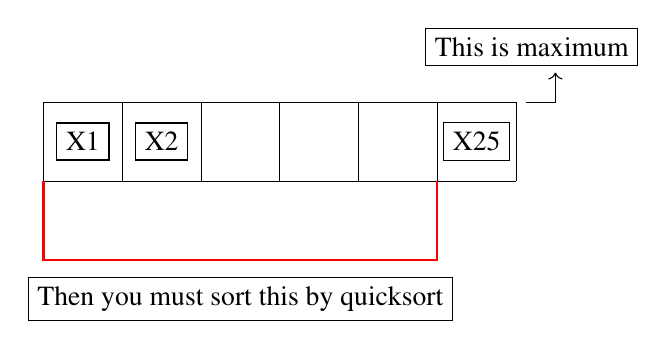
\begin{tikzpicture}
\draw[step=1cm,black,very thin] (0,0) grid (6,1)  node[anchor=north west] {};
\node[draw] at (0.5,0.5) {X1};
\node[draw] at (1.5,0.5) {X2};
\node[draw] at (5.5,0.5) {X25};
\node[draw] at (6.2,1.7) {This is maximum};
\node[draw] at (2.5,-1.5) {Then you must sort this by quicksort};
\node (A) at (6, 1) {};
\node (B) at (6.5, 1.5) {};
\draw[->, to path={-| (\tikztotarget)}]
  (A) edge (B) ;
\draw[red,thick,solid] (0,0) -- (0,-1) -- (5,-1) -- (5,0);
\end{tikzpicture} 
Minimum, \\ 
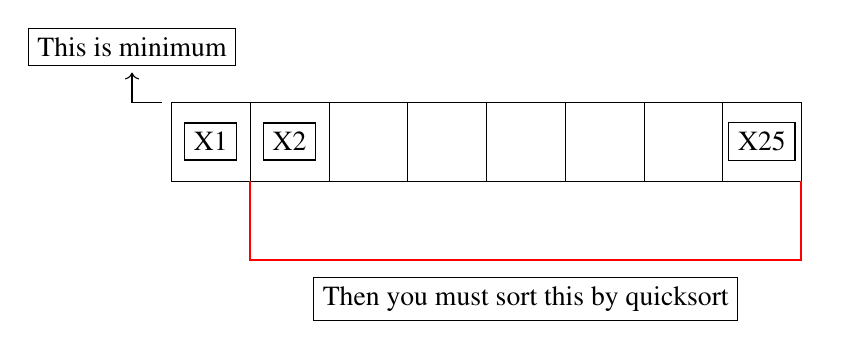
\begin{tikzpicture}
\draw[step=1cm,black,very thin] (0,0) grid (8,1)  node[anchor=north west] {};
\node[draw] at (0.5,0.5) {X1};
\node[draw] at (1.5,0.5) {X2};
\node[draw] at (7.5,0.5) {X25};
\node[draw] at (-0.5,1.7) {This is minimum};
\node[draw] at (4.5,-1.5) {Then you must sort this by quicksort};
\node (A) at (0, 1) {};
\node (B) at (-0.5, 1.5) {};
\draw[->, to path={-| (\tikztotarget)}]
  (A) edge (B) ;
\draw[red,thick,solid] (1,0) -- (1,-1) -- (8,-1) -- (8,0);
\end{tikzpicture}

%
\item $E_1$, $E_2$ are independent events such that,
\begin{align*}
    \pr{E_1} = \frac{1}{4},\,\pr{E_2|E_1} = \frac{1}{2} \text{ and } \pr{E_1|E_2} = \frac{1}{4}
\end{align*}
Define random variables $X$ and $Y$ by\\
\begin{align}
X=
\begin{cases}
1, &\text{ if $E_1$ occurs}\\
0, &\text{ if $E_1$ does not occur}
\end{cases}
\\
Y=
\begin{cases}
1, &\text{ if $E_2$ occurs}\\
0, &\text{ if $E_2$ does not occur}
\end{cases}
\end{align}
Consider the following statements
\begin{itemize}
    \item[$\alpha:$]$X$ is uniformly distributed on the set $\{0,1\}$
    \item[$\beta:$]$X$ and $Y$ are identically distributed
    \item[$\gamma:$]$\pr{X^2 + Y^2 = 1} = \frac{1}{2}$
    \item[$\delta:$]$\pr{XY=X^2Y^2} = 1$
\end{itemize}
Choose the correct combination
\begin{enumerate}[label = (\alph*)]
\begin{multicols}{2}
\setlength\itemsep{2em}
    \item $(\alpha,\beta)$
    \item $(\alpha,\gamma)$
    \item $(\beta,\gamma)$
    \item $(\gamma,\delta)$
\end{multicols}
\end{enumerate}
%
\solution
%
Since events $E_1$ and $E_2$ are independent, 
\begin{align}
    \pr{E_1E_2}&=\pr{E_1}\times\pr{E_2} \nonumber\\\nonumber\\
    \pr{E_2|E_1}&=\frac{\pr{E_1E_2}}{\pr{E_1}} = \pr{E_2} \nonumber\\ \nonumber\\
     \therefore \pr{E_2} &= \frac{1}{2}
\end{align}
\\[1000pt]
From the given information we get,\\
\begin{table}[h]
\centering
    \begin{tabular}{|c|c|c|}
        \hline
         &0 &1    \\ \hline
        $\pr{X}$ &$\frac{3}{4}$ &$\frac{1}{4}$   \\ \hline
        $\pr{Y}$ &$\frac{1}{2}$ &$\frac{1}{2}$ \\ \hline
    \end{tabular}
\caption{Probability of $X \in \{0,1\}$ and $Y \in \{0,1\}$}
\label{ma2003-80:table=1}
\end{table}
%
$F_X(x)=
\begin{cases}
1, &x\geq1\\
\frac{3}{4}, & 0\leq x \leq1\\
0, &x<0
\end{cases}$
$F_Y(y)=
\begin{cases}
1, &y\geq1\\
\frac{1}{2}, & 0\leq y \leq1\\
0, &y<0
\end{cases}$
\\
\begin{enumerate}[label=(\arabic*)]
    \item $X$ is not uniformly distributed on the set $\{0,1\}$ as it is not continuous in $\{0,1\}$ (both $X$ and $Y$ are Bernoulli Distributions).\\
    $\therefore$ Statement $\alpha$ is incorrect.\label{ma2003-80:a}\\ 
    \item Since $F_X(x)\neq F_Y(y)$, $X$ and $Y$ are not identically distributed.\\
    $\therefore$ Statement $\beta$ is incorrect.\label{ma2003-80:b}\\
    \item $\pr{X^2+Y^2=1}$\label{ma2003-80:c}
    \begin{align}
        &=\pr{X=0,Y=1}+\pr{X=1,Y=0}\nonumber\\
        &= \frac{1}{2}
    \end{align}
    $\therefore$ Statement $\gamma$ is correct.\\
    \item $\pr{XY=X^2Y^2}$\label{ma2003-80:d}
    \begin{align}
        &=\sum_{i=0}^1\sum_{j=0}^1\pr{X=i,Y=j}\nonumber\\
        &= 1
    \end{align}
    $\therefore$ Statement $\delta$ is correct.\\
\end{enumerate}
\begin{enumerate}[label=(\alph*)]
    \item This option is incorrect as statement $\alpha$ is incorrect \ref{ma2003-80:a} and statement $\beta$ is incorrect \ref{ma2003-80:b}.\\
    \item This option is incorrect as statement $\gamma$ is correct \ref{ma2003-80:c} but statement $\alpha$ is incorrect \ref{ma2003-80:a}.\\
    \item This option is incorrect as statement $\gamma$ is correct \ref{ma2003-80:c} but statement $\beta$ is incorrect \ref{ma2003-80:b}.\\
    \item This option is correct as statement $\gamma$ is correct \ref{ma2003-80:c} and statement $\delta$ is correct \ref{ma2003-80:d}.\\
\end{enumerate}
$\therefore$ Option (d), $(\gamma,\delta)$, is the answer.
%
\item Arrivals at a telephone booth are considered to be Poisson, with an average time of 10 minutes between successive arrivals.The length of a phone call is distributed exponentially with mean 3 minutes.The probability that an arrival does not have to wait before service is
\begin{enumerate}
    \item{0.3}
    \item{0.5}
    \item{0.7}
    \item{0.9}
\end{enumerate}
%
\solution

Let X be a random variable with values equal to time between successive calls(in minutes) which is a Poisson distribution with mean of 10.\\
\begin{align}
\implies \pr{X=x}=\frac{e^{-10}\times 10^{x}}{x!} \quad(x=1,2,3,...)
\end{align}
Let Y be a random variable with values equal to length of a phone call which is an exponential distribution with mean 3.
\begin{align}
\implies f_{Y}(y)=\begin{cases}\frac{e^{\frac{-y}{3}}}{3}\quad &\text{for}\,\,x \geq 0  \\
0 \quad &\text{for}\,\, x<0
\end{cases}\\
\implies \pr{Y \leq y}=F_{Y}(y)&=\int_{-\infty}^{y}f_{Y}(y)dy\\
           &=\int_{0}^{y}\frac{e^{\frac{-y}{3}}}{3}\\
           &=1-e^{\frac{-y}{3}}
\end{align}
Probability that an arrival does not have to wait is $\pr{Y\leq X}$
\begin{align}
\pr{Y \leq X}&=\sum_{x=0}^{x=\infty}\pr{Y \leq x}\pr{X=x}\\
             &=\sum_{x=0}^{x=\infty}(1-e^{\frac{-x}{3}})\times \brak{\frac{e^{-10}\times 10^{x}}{x!}}\\
             &=e^{-10}\brak{\sum_{x=0}^{x=\infty}\frac{10^{x}}{x!}-\sum_{x=0}^{x=\infty}\frac{10^{x}e^{\frac{-x}{3}}}{x!}}\\
             &=e^{-10}\brak{e^{10}-\sum_{x=0}^{x=\infty}\frac{e^{\brak{\log_{e}10-\frac{1}{3}}x}}{x!}}\\
             &=1-e^{-10}\brak{e^{e^{\brak{log_{e}10-\frac{1}{3}}}}}\\
             &=0.941
\end{align}
Hence option (4) is correct.
%
\item  Let Z be an exponential random variable with mean 1. That is, the cumulative distribution function of Z is given by 
\begin{align}
    F_Z(x) =
    \begin{cases}
    1 - {e^{-x}}, & if\ x \ge 0\\
    0, & if\ x<0.
    \end{cases}
\end{align}
Then Pr{(Z>2 | Z>1)}, rounded off to two decimal places, is equal to 
%
\solution


 \begin{align}
 Pr{(Z>2 | Z>1)} &= \dfrac{Pr{((Z>2),(Z>1))}}{Pr{(Z>1)}} \\
                 &= \dfrac{Pr{(Z>2)}}{Pr{(Z>1)}} \\
                 &= \dfrac{1 - Pr{(Z \le 2)}}{1 - Pr{(Z \le 1)}} \\
                 &= \dfrac{e^{-2}}{e^{-1}} \\
                 &= e^{-1} = 0.3679
\end{align}

%
\item A coin is tossed 4 times. What is the probability of getting heads exactly three times ?
\begin{enumerate}
    \item $\frac{1}{4}$ 
    \item $\frac{3}{8}$
    \item $\frac{1}{2}$
    \item $\frac{3}{4}$
    
\end{enumerate}
%
\solution

In an experiment of tossing a coin $n$( = 4) times, random variable  $X \in \lbrace 0,1,2,3 \rbrace$ follows binomial distribution.\\
The binomial distribution formula is:
\begin{align}
 \Pr( X=k ) &= \comb{n}{k} \times p^k \times (1- p)^{n - k}
\end{align}
Where:
\begin{table}[h]
    \centering
    \resizebox{\columnwidth}{!}{%
    \begin{tabular}{|r|c|}\hline
    $k$ &  total number of “successes” \\ \hline
    $p$ & probability of a success on an individual trial\\ \hline
    $n$ & number of trials = 3 \\ \hline
\end{tabular}}
\caption{The binomial distribution formula}
    \label{me2008-4:table:0}
\end{table}
Let $X$ denote the number of heads
\begin{align}
    \Pr(X=3) &=  \comb{4}{3} \times \left(\frac{1}{2}\right)^3 \times \left(1- \frac{1}{2}\right)^{4 - 3}\\
    &= \frac{1}{4}
\end{align}
Correct option is 1.
%
\item There are two identical locks, with two identical keys, and the keys are among the six different ones which a person carries in his pocket. In a hurry he drops one key somewhere. Then the probability that the locks can still be opened by drawing one key at random is equal to?
%
\solution

\begin{align*}
\text{Let } &E_1  &&\text{denote that he drops the needed key}\\
&E_2  &&\text{denote that he drops an unwanted key}\\
&A  &&\text{denote the event of opening the locks}
\end{align*}
\begin{align}
\pr{E_1} &= \frac{1}{3}\\
\pr{E_2} &= \frac{2}{3}\\
\pr{A|E_1} &= \frac{1}{5}\\
\pr{A|E_2} &= \frac{2}{5}
\end{align}\\
Hence by total probability rule,
\begin{align}
\pr{A} &= \pr{E_1}\times \pr{A|E_1} + \pr{E_2}\times \pr{A|E_2}\\
&= \frac{1}{3}\times\frac{1}{5} + \frac{2}{3}\times\frac{2}{5}
\end{align}
Hence, the probability that the locks can be opened is $\frac{1}{3}$
%
\item An automobile plant contracted to buy shock absorbers from two suppliers X and Y. X supplies 60\% and y supplies 40\% of the shock absorbers. All shock absorbers are subjected to a quality test.The ones that pass the quality test are considered reliable. Of X's shock absorbers are 96\% are reliable. Of Y's shock absorbers 72\% are reliable The probability that a randomly chosen shock absorber which is found to be reliable is made by Y is
\begin{enumerate}
    \item 0.288
    \item 0.334
    \item 0.667
    \item 0.720
\end{enumerate}
%
\solution

Let A and B be two random variables that take values from the set \{0,1\}.\newline
A:
\begin{itemize}
    \item A=0 $\rightarrow$ \text{shock absorber is from X}
    \item A=1 $\rightarrow$ \text{shock absorber is from Y}
\end{itemize}
B:
\begin{itemize}
    \item B=0 $\rightarrow$ \text{shock absorber is not reliable}
    \item B=1 $\rightarrow$ \text{shock absorber is reliable}
\end{itemize}
\begin{table}[h!]
    \centering
    \begin{tabular}{|c|c|c|}
        \hline
        $x_i$ & Description & P(A=$x_i$)\\
        \hline
        0 & Shock absorber is from X & 0.6\\
        1 & Shock absorber is from Y & 0.4\\
        \hline
    \end{tabular}
    \caption{Values taken by X}
    \label{me2012-64:tab:1}
\end{table}
Given,
\begin{align}
    \pr{B=1|A=0} &= 0.96\\
    \pr{B=1|A=1} &= 0.72
\end{align}
Using the fact that \pr{E|F} = $\frac{\pr{E+F}}{\pr{F}}$,
\begin{multline}
    \pr{\brak{B=1}+\brak{A=0}} = \pr{B=1|A=0} \times \\
    \pr{A=0}
\end{multline}
\begin{align}
\pr{\brak{B=1}+\brak{A=0}} &= 0.576 \\
\text{Similarly,}\label{me2012-64:2.0.5} \pr{\brak{B=1}+\brak{A=1}} &= 0.288 
\end{align}
Since the events (A=0) and (A=1) are mutually independent and mutually exhaustive, we can say that 
\begin{multline}
    \pr{B=1} = \pr{\brak{B=1}+\brak{A=0}} + \\
    \pr{\brak{B=1}+\brak{A=1}}.
\end{multline}
\begin{equation}\label{me2012-64:(2.0.7)}
    \implies \pr{B=1} = 0.864
\end{equation}
We need to find \pr{A=1|B=1}
\begin{align}
    \pr{A=1|B=1} = \frac{\pr{\brak{A=1}+\brak{B=1}}}{\pr{B=1}}
\end{align}
Substituting values from \eqref{me2012-64:2.0.5} \eqref{me2012-64:(2.0.7)}, we get
\begin{align}
    \pr{A=1|B=1} &= \frac{0.288}{0.864} \\
    \implies \pr{A=1|B=1} &= 0.3333333 \\
    \implies \pr{A=1|B=1} &= 0.334
\end{align}
%
\item A box contains 15 blue balls and 45 black balls. If two balls are selected randomly, without replacement, the probability of an outcome in which the first ball selected is a blue ball and the second ball selected is a black ball, is .....

    \begin{enumerate}[label=\arabic*.]
        \item \Large$\frac{3}{16}$ \\
        \item $\frac{45}{236}$
        \item $\frac{1}{4}$ \\
        \item $\frac{3}{4}$
    \end{enumerate}
%
\solution

Let $X_1 \text{ and } X_2 \in \cbrak{0,1}$ where 0 represents a black and 1 represents a blue ball.
\begin{enumerate}[label=\alph*)]
    \item Probability of picking a blue ball
      \begin{align}
        \pr{X_1=1} = \frac{15}{60} = \frac{1}{4}
      \end{align}
    \item Probability of picking a black ball given a blue ball is picked
      \begin{align}
        \pr{X_2=0|X_1=1} = \frac{45}{59}
      \end{align}
    \item Probability that first ball is blue and second ball is black
      \begin{multline}
        \pr{X_1=1,X_2=0}= \\\pr{X_1=1} \times \pr{X_2=0|X_1=1} 
      \end{multline}
    \begin{align}
       &= \frac{1}{4} \times \frac{45}{59}\\ 
       &= \frac{45}{236} 
    \end{align}
\end{enumerate}
$\therefore$ Option 2 is correct.

%
\item A single die is thrown twice. What is the probability that the sum is neither 8 or 9?
    \begin{enumerate}[label=(\alph*)]
        \item \large$\frac{1}{9}$
        \item \large$\frac{5}{36}$
        \item \large$\frac{1}{4}$
        \item \large$\frac{3}{4}$
    \end{enumerate}
%
\solution

Let $X \in \{0,1\}$ be the random variable, where X=0 represents that we get sum to be 8 or 9 and X=1 represents that we get sum between 2 and 12 except 8 and 9.\\
Total number of possible outcomes is :
\begin{equation}
    N = {\comb{6}{1}}\times{\comb{6}{1}} = 36
\end{equation}
 
Probability that the sum is neither 8 or 9 
\begin{equation}\label{me2005-38:eq:2}
  \pr{X=1} = 1-\pr{X=0}
\end{equation}
 Only 9 outcomes are favourable to the occurrence of X=0 .\\
Probability of getting sum 8 or 9 is :
\begin{equation}
    \pr{X=0} = \frac{9}{36}
             = \frac{1}{4}
\end{equation}
Substituting value in \eqref{me2005-38:eq:2} , we get
\begin{equation}
 \pr{X=1} = 1- \frac{1}{4}
          = \frac{3}{4}   
\end{equation}
Hence, the correct option is (d) \large$\frac{3}{4}$
%
\item A box contains 2 washers, 3 nuts and 4 bolts. Items are drawn from the box at random one at a time without replacement. The probability of drawing 2 washers first followed by 3 nuts and subsequently 4 bolts is
%
    \begin{enumerate}[label=(\Alph*)]
        \item \large$\frac{2}{315}$
        \item \large$\frac{1}{630}$
        \item \large$\frac{1}{1260}$
        \item \large$\frac{1}{2520}$
    \end{enumerate}
%
%
\solution

Let $X\in\{0,1,2\}$ be the random variable such that X=0 represents that we draw 2 washers, X=1 represents that we draw 3 nuts and X=2 represents that we draw 4 bolts, continuously without replacement. \\
Total number of objects :
\begin{equation}
    N = 2+ 3+ 4 = 9
\end{equation}
Probability of occurrence of X=0 :
\begin{align}
    \pr{X=0} =& \dfrac{\comb{2}{2}}{\comb{9}{2}} \\
     =& \dfrac{1}{36}    
\end{align}
Total number of objects after occurrence of X=0 :
\begin{equation}
    N = 3+ 4 = 7
\end{equation}
Probability of occurrence of X=1 given that X=0 has already occurred :
\begin{align}
    \pr{X=1|X=0} =& \dfrac{\comb{3}{3}}{\comb{7}{3}}\\
   =& \dfrac{1}{35} 
\end{align}
Total number of objects after occurrence of X=0 and X=1 :
\begin{equation}
    N = 4 
\end{equation}
Probability of occurrence of X=2 given that X=0 and X=1 has already occurred :
\begin{align}
    \pr{X=2|(X=0,X=1)} =&\dfrac{\comb{4}{4}}{\comb{4}{4}} \\
     =& 1
\end{align}
Using Multiplication law of probability,\\ Required probability is given by :
\begin{multline}
    \pr{X=0 , X=1 , X=2} \\
      = \pr{X=0}\times \pr{X=1|X=0}\\\times \pr{X=2|(X=0,X=1)}
    \end{multline}
    
\begin{align}
\implies\pr{X=0 , X=1 , X=2} =& \frac{1}{36}\times\frac{1}{35}\times1 \\
=& \frac{1}{1260}
\end{align}
$\therefore$ The correct option is (C) \large $\frac{1}{1260}$.

%
\item  Let $U$ and $V$ be two independent zero mean Gaussian random variables of variances $\frac{1}{4}$ and $\frac{1}{9}$ respectively. The probability $\pr{3V\geq2U }$ is
\begin{enumerate}
    \item $4/9$
    \item $1/2$
    \item $2/3$
    \item $5/9$
\end{enumerate}
%
\solution

$U$ and $V$ are independent random variables,
For $V$, $\mu_V=0$, and $\sigma_V^2=\frac{1}{9}$
\begin{align}
    V\sim N\brak{0,\frac{1}{9}}
\end{align}
For $U$, $\mu_U=0$, and $\sigma_U^2=\frac{1}{4}$
\begin{align}
    U\sim N\brak{0,\frac{1}{4}}
\end{align}
Let,
\begin{align}
    Z=3V-2U\\
    Z\sim N\brak{\brak{3\mu_V-2\mu_U}, \brak{(3)^2\sigma_U^2+(2)^2\sigma_V^2}}\\
    Z\sim N\brak{0,9\times\frac{1}{9}+4\times\frac{1}{4}}\\
    Z\sim N\brak{0,2}
\end{align}
For $Z$, $\mu=0$, and $\sigma^2=2$.
By Gaussian Distribution,
Let $X$ is standard normal variable,
\begin{align}
    X=\frac{Z-\mu}{\sigma}\\
    \pr{Z\geq0}=\pr{X\sigma+\mu\geq0}\\
    \pr{Z\geq0}=\pr{X\brak{\sqrt{2}}+0\geq0}\\
    \pr{Z\geq0}=\pr{X\geq0}\\
    \pr{Z\geq0}=Q\brak{0}
\end{align}
where $Q(x)$ is the $Q-function$,
\begin{align}
    Q\brak{0}=\frac{1}{2}\\
    \pr{Z\geq0}=\frac{1}{2}\\
    \pr{3V-2U\geq0}=\frac{1}{2}\\
    \pr{3V\geq2U}=\frac{1}{2}
\end{align}
Option (B) is correct.
%
\item Two random variables X and Y are distributed according to
\begin{align}
 f_{X,Y}(x,y)=\begin{cases} 
      x+y & 0\leq x\leq 1, 0\leq y\leq 1 \\
      0 & otherwise
  \end{cases}
\end{align}
The probability $\Pr(X+Y\leq 1)$ is 
%
\solution

\begin{align}
Pr(X+Y\leq 1)&=\Int_{0}^{1} \Int_{0}^{1-y}f_{X,Y}(x,y) \,dx\,dy
\\
&=\Int_{0}^{1} \Int_{0}^{1-y}(x+y)\,dx\,dy
\\
&=\Int_{0}^{1} \brak{\brak{\dfrac{x^2}{2}+xy} \Big|_{0}^{1-y}}\,dy
\\
&=\Int_{0}^{1} \brak{\dfrac{1-y^2}{2} }\,dy
\\
&= \brak{\dfrac{y}{2}-\dfrac{y^3}{6}}\Big|_{0}^{1}\,dy
\\
&=\dfrac{1}{3}
\end{align}
Therefore, required probability is $=\dfrac{1}{3}$
%
\item A box contains 4 red balls and 6 black balls. Three balls are selected randomly from the box one after another, 
without replacement. What is the probability that the selected set contains one red ball and two black balls?\bigskip
\begin{enumerate}\itemsep0.3cm
    \item $\displaystyle{\frac{1}{20}}$
    \item $\displaystyle{\frac{1}{12}}$
    \item $\displaystyle{\frac{3}{10}}$
    \item $\displaystyle{\frac{1}{2}}$
\end{enumerate}
%
\solution

This problem uses Hyper-Geometric distribution which involves selection of certain number of \newline successes from a given sample without replacement.
\begin{itemize}
    \item Number of Red balls = 4
    \item Number of Black balls = 6
\end{itemize}
Let M be a variable representing the number of black balls in a selection of 3 balls.
M has a \newline Hyper-Geometric probability mass function:
\begin{equation}
    p_M(k) = \pr{M = k} = \frac{\comb{K}{k} \times \comb{N-K}{n-k}}{\comb{N}{n}}
\end{equation}
Here Success refers to selecting a black ball,
\begin{table}[!ht]
    \begin{center}
        \resizebox{\columnwidth}{!}
        {
            \begin{tabular}{|c|c|c|}
                \hline
                K & Total successes in population & 6\\
                \hline
                N & Population size & 6 + 4 = 10\\
                \hline
                k & Total observed successes & 2\\
                \hline
                n & Number of draws & 3\\
                \hline
            \end{tabular}
        }
    \end{center}
\end{table}
Probability that the selected set contains 2 black balls and 1 red ball = $\pr{M = 2}$
\begin{align}
    \pr{M = 2} = \hspace{0.2cm}& \frac{\comb{K}{2} \times \comb{N-K}{n-2}}{\displaystyle{\comb{N}{n}}}\\[0.3cm]
               = \hspace{0.2cm}& \frac{\comb{6}{2} \times \comb{10-6}{3-2}}{\displaystyle{\comb{10}{3}}}\\[0.3cm]
               = \hspace{0.2cm}& \frac{\comb{6}{2} \times \comb{4}{1}}{\displaystyle{\comb{10}{3}}}\\[0.3cm]
               = \hspace{0.2cm}& \frac{15 \times 4}{120}\\[0.3cm]
               = \hspace{0.2cm}& \frac{1}{2}
\end{align}
So the probability that the selected set of 3 balls contain 2 black balls and 1 red ball is $\displaystyle{\frac{1}{2}}$.
%
\item Suppose a fair six-sided die is rolled once. If the value on the die is 1,2, or 3, the die is rolled a second time. What is the probability that the sum total of values that turn up is at least 6?
\begin{enumerate}
    \item 10/21
    \item 5/12
    \item 2/3
    \item 1/6
\end{enumerate}
%
\solution

Let us define a random variable $X \in \cbrak{0,1}$\\
\begin{table}[ht]
    \centering
    \begin{tabular}{|c|c|}
    \hline
    X=0 & Getting 1,2, or 3 on first roll\\
    \hline
    X=1 & Getting the sum total of values at least 6\\
    \hline
    \end{tabular}
    \caption{Random Variables}
    \label{cs2012-33:tab:Random Variables}
\end{table}

Probability of getting 1,2, or 3 on first roll is given by,
\begin{align}
    \pr{X=0}&=\cfrac{3}{6}= \cfrac{1}{2}\\
\end{align}
Probability of getting sum total of 6 on first roll is given by,
\begin{align}   
    \pr{X=1}&= \cfrac{1}{6}\\
\end{align} 
Probability of getting sum total of 6 after getting 1,2,or,3 in first roll is given by,
\begin{align}    
    \pr{X=1|X=0}&=\cfrac{9}{18}= \cfrac{1}{2}
\end{align}
Now,probability of getting sum total of 6 and getting 1,2,or,3 in first roll is given by,
\begin{align}
    \pr{X=1 , X=0}&=\pr{X=1|X=0}\times\pr{X=0}\\
                     &=\cfrac{1}{2} \times \cfrac{1}{2}\\
                     &=\cfrac{1}{4}
\end{align}
\begin{table}[ht]
    \centering
    \begin{tabular}{|c|c|c|c|}
    \hline
    X & X=0 & X=1 & X=1$|$X=0\\
    \hline
    $\pr{X}$ & $\cfrac{1}{2}$ & $\cfrac{1}{6}$ & $\cfrac{1}{2}$\\
    \hline
    \end{tabular}
    \caption{Probability distribution table}
    \label{cs2012-33:tab:Probability distribution table}
\end{table}
\newline
The probability that the sum total of values that turn up is at least 6 is given by
\begin{align}
    \pr{X=1 , X=0} + \pr{X=1} &= \cfrac{1}{4} + \cfrac{1}{6}\\
    &=\cfrac{5}{12}
\end{align}
%
\item  The probability that the top and bottom cards of a randomly shuffled deck are both aces is
\begin{description}
\item[$\brak{A}$]$\dfrac{4}{52}\times\dfrac{4}{52}$ \\
\item[$\brak{B}$]$\dfrac{4}{52}\times\dfrac{3}{52}$ \\
\item[$\brak{C}$]$\dfrac{4}{52}\times\dfrac{3}{51}$ \\
\item[$\brak{D}$]$\dfrac{4}{52}\times\dfrac{4}{51}$ \\
\end{description}
%
\solution

Let the following random variables and their values denote:
\begin{align*}
    A : \text{Top card is an ace} &= 1\\
    B : \text{Bottom card is an ace} &=1
\end{align*}
\begin{align}
    \pr{A=1} &= \frac{4}{52} \label{cs1996-32:eq1} \\
    \pr{B = 1|A = 1} &= \frac{3}{51} \label{cs1996-32:eq2}
\end{align}
Applying Bayes Theorem, 
\begin{align}
    \pr{B = 1, A = 1} &= \pr{B = 1|A = 1} \pr{A = 1}\\
\intertext{from \eqref{cs1996-32:eq1} and \eqref{cs1996-32:eq2},}
    \pr{B = 1, A = 1} &=   \frac{4}{52} \times\frac{3}{51}
\end{align}
\\The correct option is \textbf{Option (C)}.

%
\item A six-faced fair dice is rolled five times. The probability (in percentage ) of obtaining “ONE” at least four times is 
\begin{enumerate}
    \item 33.3
    \item 3.33
    \item 0.33
    \item 0.0033
\end{enumerate}
%
\solution

Let X be the random variable denoting the number the times "ONE" is obtained when a six-faced die is rolled n-times.X follows binomial distribution.\\
From binomial Distribution,
\begin{align*}
\Pr(X=k)={\comb{n}{k}} p^k(1-p)^{n-k}\hspace{1cm} k=0,1,....,n
\end{align*}
For this given problem $ n=5,p=\frac{1}{6}$ for a six-faced die\\
The probability (in percentage ) of obtaining “ONE” at least four times is $\Pr(X\geq4)\times100$
\begin{align*}
&\Pr(X\geq4)=\sum_{k=4}^{5}\Pr(X=k)\\
&=\Pr(X=4)+\Pr(X=5)\\
&={\comb{5} {4}}\frac{5}{6^5}+{\comb{5} {5}}\frac{1}{6^5}\\
&=\frac{26}{6^5}
\end{align*}
Probability in percentage is,
\begin{align*}
    &=\frac{26}{6^5}\times100\\
    &=0.334
\end{align*}
Option c is correct.
%
\item Let $X$ and $Y$ be two statistically independent random variables uniformly
distributed in the ranges $(-1,1)$ and $(-2,1)$ respectively. Let $Z = X + Y.$ then the probability that $[Z\leq-2]$ is
\begin{enumerate}[label=\alph*)]
\item zero
\item $\frac{1}{6}$
\item $\frac{1}{3}$
\item $\frac{1}{12}$
\end{enumerate}
%
\solution

The pdf of $Z(=X+Y)$ will be convolution of pdf of $X$ and pdf of $Y$ as shown below.
\begin{align}
f_{x}( x)\times f_{y}(y)=f_{z}(z)
\end{align}
\tikzset{every picture/.style={line width=0.5pt}} %set default line width to 0.75pt        
\begin{tikzpicture}[x=0.45pt,y=0.5pt,yscale=-1,xscale=1]
%uncomment if require: \path (0,300); %set diagram left start at 0, and has height of 300
%Straight Lines [id:da7994322016020907] 
\draw [line width=0.75]    (65.3,280.6) -- (580.3,280.6) ;
%Straight Lines [id:da6298726397789813] 
\draw [line width=0.75]    (321.8,68.4) -- (322.8,280.6) ;
%Shape: Right Angle [id:dp8023791863547924] 
\draw  [color={rgb, 255:red, 0; green, 0; blue, 0 }  ,draw opacity=1 ][line width=1.5]  (254.8,168.6) -- (389.8,168.6) -- (389.8,279) ;
%Straight Lines [id:da07001326664875096] 
\draw [line width=1.5]    (254.8,168.6) -- (254.8,279) ;
% Text Node
\draw (403,152.4) node [anchor=north west][inner sep=0.75pt]    {$\dfrac{1}{2}$};
% Text Node
\draw (240,285.4) node [anchor=north west][inner sep=0.75pt]    {$-1$};
% Text Node
\draw (385,282.4) node [anchor=north west][inner sep=0.75pt]    {$1$};
% Text Node
\draw (318,283.4) node [anchor=north west][inner sep=0.75pt]    {$0$};
% Text Node
\draw (303,44.4) node [anchor=north west][inner sep=0.75pt]    {$f_{x}( x)$};
% Text Node
\draw (590,269.4) node [anchor=north west][inner sep=0.75pt]    {$x$};
\end{tikzpicture}
\tikzset{every picture/.style={line width=0.5pt}} %set default line width to 0.75pt        
\begin{tikzpicture}[x=0.45pt,y=0.5pt,yscale=-1,xscale=1]
%uncomment if require: \path (0,300); %set diagram left start at 0, and has height of 300
%Straight Lines [id:da7994322016020907] 
\draw [line width=0.75]    (65.3,280.6) -- (580.3,280.6) ;
%Straight Lines [id:da6298726397789813] 
\draw [line width=0.75]    (321.8,68.4) -- (322.8,280.6) ;
%Shape: Right Angle [id:dp8023791863547924] 
\draw  [color={rgb, 255:red, 0; green, 0; blue, 0 }  ,draw opacity=1 ][line width=1.5]  (267.8,168.6) -- (389.8,168.6) -- (389.8,279) ;
%Straight Lines [id:da07001326664875096] 
\draw [line width=1.5]    (267.8,168.6) -- (189.8,169.4) -- (189.8,280) ;
% Text Node
\draw (403,152.4) node [anchor=north west][inner sep=0.75pt]    {$\dfrac{1}{3}$};
% Text Node
\draw (240,282.4) node [anchor=north west][inner sep=0.75pt]    {$-1$};
% Text Node
\draw (385,282.4) node [anchor=north west][inner sep=0.75pt]    {$1$};
% Text Node
\draw (318,283.4) node [anchor=north west][inner sep=0.75pt]    {$0$};
% Text Node
\draw (303,44.4) node [anchor=north west][inner sep=0.75pt]    {$f_{y}( y)$};
% Text Node
\draw (590,269.4) node [anchor=north west][inner sep=0.75pt]    {$y$};
% Text Node
\draw (175,280.4) node [anchor=north west][inner sep=0.75pt]    {$-2$};
\end{tikzpicture}
\tikzset{every picture/.style={line width=0.5pt}} %set default line width to 0.75pt        
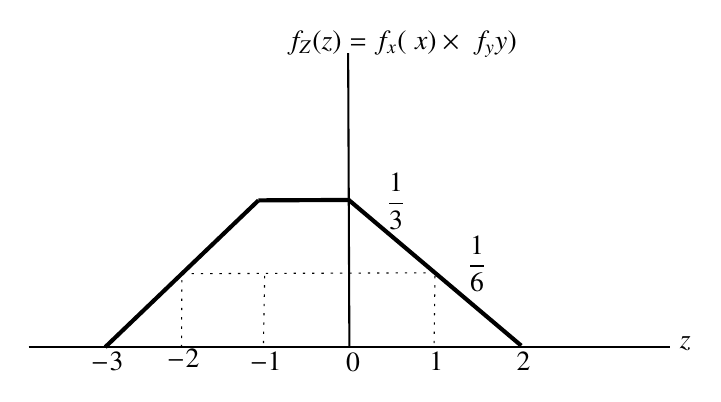
\begin{tikzpicture}[x=0.45pt,y=0.5pt,yscale=-1,xscale=1]
%uncomment if require: \path (0,300); %set diagram left start at 0, and has height of 300
%Straight Lines [id:da7994322016020907] 
\draw [line width=0.75]    (65.3,280.6) -- (580.3,280.6) ;
%Straight Lines [id:da6298726397789813] 
\draw [line width=0.75]    (321.8,68.4) -- (322.8,280.6) ;
%Straight Lines [id:da3048610517318646] 
\draw [line width=1.5]    (249.8,174.8) -- (322.3,174.5) ;
%Straight Lines [id:da21348606992409946] 
\draw [line width=1.5]    (249.8,174.8) -- (126.8,280.8) ;
%Straight Lines [id:da9537386999126634] 
\draw [line width=1.5]    (322.3,174.5) -- (460.8,279.8) ;
%Straight Lines [id:da7472472432945507] 
\draw  [dash pattern={on 0.84pt off 2.51pt}]  (391.55,227.15) -- (188.3,227.8) ;
%Straight Lines [id:da7478392311577124] 
\draw  [dash pattern={on 0.84pt off 2.51pt}]  (188,281) -- (188.3,227.8) ;
%Straight Lines [id:da11363593871174427] 
\draw  [dash pattern={on 0.84pt off 2.51pt}]  (253.8,278) -- (254.8,228) ;
%Straight Lines [id:da30914849700103675] 
\draw  [dash pattern={on 0.84pt off 2.51pt}]  (390.8,278) -- (391.55,227.15) ;
% Text Node
\draw (350,153.4) node [anchor=north west][inner sep=0.75pt]    {$\dfrac{1}{3}$};
% Text Node
\draw (241,282.4) node [anchor=north west][inner sep=0.75pt]    {$-1$};
% Text Node
\draw (385,282.4) node [anchor=north west][inner sep=0.75pt]    {$1$};
% Text Node
\draw (318,283.4) node [anchor=north west][inner sep=0.75pt]    {$0$};
% Text Node
\draw (271,50.4) node [anchor=north west][inner sep=0.75pt]    {$f_{Z}( z) =f_{x}( \ x) \times \ f_{y} y)$};
% Text Node
\draw (175,280.4) node [anchor=north west][inner sep=0.75pt]    {$-2$};
% Text Node
\draw (114,282.4) node [anchor=north west][inner sep=0.75pt]    {$-3$};
% Text Node
\draw (455,282.4) node [anchor=north west][inner sep=0.75pt]    {$2$};
% Text Node
\draw (586,271.4) node [anchor=north west][inner sep=0.75pt]    {$z$};
% Text Node
\draw (415,198.4) node [anchor=north west][inner sep=0.75pt]    {$\dfrac{1}{6}$};
\end{tikzpicture}
Now
\begin{align}
\pr{Z \leq z} &=\int_{-\infty}^{z} f_{Z}(z) d z \\
\pr{Z \leq-2} &=\int_{-\infty}^{-2} f_{Z}(z) d z \\
&=\text {Area }[z \leq-2] \\
&=\frac{1}{2} \times \frac{1}{6} \times 1=\frac{1}{12}
\end{align}
Hence $(\mathrm{D})$ is correct option.
%
\item Let P(E) denote the probability of the event E. Given P(A)=1, P(B)=$\frac{1}{2}$, the values of P(A$|$B) and P(B$|$A) respectively are
%
\begin{enumerate}
    \item $\frac{1}{4},\frac{1}{2}$
    \item $\frac{1}{2},\frac{1}{4}$
    \item $\frac{1}{2},1$
    \item $1,\frac{1}{2}$
\end{enumerate}
%
\solution
Applying Boolean Logic,\begin{align}P(A)=1 \implies A=1\label{cs2003-3:eq1}\\ P(A|B)=\frac{P(AB)}{P(B)} \end{align} Using \eqref{cs2003-3:eq1}, \begin{align} P(A|B)&=\frac{P(1\times B)}{P(B)}\\ &=\frac{P(B)}{P(B)}=1\\ P(B|A)&=\frac{P(AB)}{P(A)}\\ &=\frac{P(B)}{P(A)}=\dfrac{\frac{1}{2}}{1}=\frac{1}{2}\end{align}Hence the correct answer is option 4).

%

\item Probability density function $p(x)$ of random variable x is as shown below. The value of a is
\begin{enumerate}[label=\Alph*)]
    \item $\frac{2}{c}$
    \item $\frac{1}{c}$
    \item $\frac{2}{(b+c)}$
    \item $\frac{1}{(b+c)}$
\end{enumerate}
\begin{figure}[!ht]
\centering
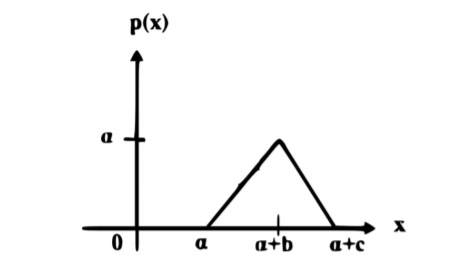
\includegraphics[width=\columnwidth]{solutions/in/2006/2/figures/convolution.png}
\caption{PDF}
\label{in2006-2:fig:convolution}
\end{figure}
%
\solution


Let $Y_1$ and $Y_2$ be two independent and identically distributed (IID) uniform random variables.\\
Let X be a random variable such that
\begin{align}
    X = Y_1 + Y_2
\end{align}
Let
\begin{align}
    p_{Y_1}\brak{y} &= \Pr\brak{Y_1=y} \\
    p_{Y_2}\brak{y} &= \Pr\brak{Y_2=y} \\
    p_X\brak{x} &= \Pr\brak{X=x}
\end{align}
be the probability densities of random variables $Y_1, Y_2$ and $X$. \\
$Y_1$ and $Y_2$ lie in the range \brak{\frac{-c}{4},\frac{c}{4}}, therefore, the PDF for $Y_1$ and $Y_2$,
\begin{align}
p_{Y_1}\brak{y} = p_{Y_2}\brak{y} = 
\begin{cases}
\frac{2}{c} &  \frac{-c}{4} \le y \le \frac{c}{4}\\
0 & \text{otherwise}
\end{cases}
\end{align}

The density of X is obtained by convolution of $Y_1$ and $Y_2$
\begin{align}
p_X\brak{x} = p_{Y_1}(x)*p_{Y_2}(x)
\end{align}
where $*$ denotes the convolution operation. Since convolution operation is time invariant, 
\begin{multline}
    p_X\brak{x-t} = p_{Y_1}(x-t)*p_{Y_2}(x) \\ = p_{Y_1}(x)*p_{Y_2}(x-t)
\end{multline}
On time shifting $Y_1$ by shifting factor $t=a+\frac{c}{2}$, 
\begin{align}
    p_X\brak{x-\brak{a+\frac{c}{2}}} =  p_{Y_1}\brak{x-\brak{a+\frac{c}{2}}}*p_{Y_2}\brak{x}
\end{align}
Thus, the PDF of time shifted X obtained by convolution is,
\begin{align}
p_x = 
\begin{cases}
\frac{4}{c^2}\brak{x-a} & a \le x \le a+\frac{c}{2}\\
\frac{4}{c^2}\brak{a+c-x} & a+\frac{c}{2} \le x \le a+c \\
0 & \text{otherwise}
\end{cases}
\end{align}

On comparing the parameters of PDF of time shifted X with that in the question, we have

\begin{align}
    b=\frac{c}{2}\\
    a=\frac{2}{c}
\end{align}
\rightline{Answer : Option A}


\begin{figure}[!ht]
\centering
\includegraphics[width=\columnwidth]{solutions/in/2006/2/figures/con6.png}
\caption{PDF of time shifted X}
\label{in2006-2:fig:con6}
\end{figure}
The following are some observations: 
\begin{enumerate}
    \item The sum of two equally distributed random variables will lead to a triangular probability density
    \item The two uniformly distributed random variables lie in the range $\brak{\frac{-c}{4},\frac{c}{4}}$ and $\brak{\frac{2}{c}+\frac{c}{4} , \frac{2}{c}+\frac{3c}{4}}$. \\
     $ \because X = Y_1 + Y_2$ the range of X is thus $\brak{\frac{2}{c},\frac{2}{c}+c}$
    \item On time shifting $Y_1$ to the right by a factor $a+\frac{c}{2}$, the convoluted PDF of X also shifts by the same factor without any change in it's width.
\end{enumerate}

Fig \ref{in2006-2:fig:sim3} and Fig \ref{in2006-2:fig:sim4} are the plots of PDF and CDF obtained by taking c=2
\begin{figure}[!ht]
\centering
\includegraphics[width=\columnwidth]{solutions/in/2006/2/figures/sim3.png}
\caption{PDF of $Y_1, Y_2$ and X}
\label{in2006-2:fig:sim3}
\end{figure}
\begin{figure}[!ht]
\centering
\includegraphics[width=\columnwidth]{solutions/in/2006/2/figures/sim4.png}
\caption{CDF of X}
\label{in2006-2:fig:sim4}
\end{figure}




%
\item The PDF of a Gaussian random variable X is given by 
P$_{X}(x) = \dfrac{1}{3\sqrt{2\pi}}e^{\dfrac{-(x-4)^{2}}{18}}$.The probability of the event { X = 4} is\\
\begin{enumerate}
    \item  $\dfrac{1}{2}$\\
    \item  $\dfrac{1}{3\sqrt{2\pi}}$\\
    \item  0\\
    \item  $\dfrac{1}{4}$\\
\end{enumerate}
%
\solution
Given PDF function is
\begin{align}
  P_{X}(x) &= \dfrac{1}{3\sqrt{2\pi}}e^{\dfrac{-(x-4)^{2}}{18}}
\end{align}
Since continuous probability functions are defined for an infinite number of points over a continuous interval, the probability at a single point is always zero.
\begin{align}
    \pr{x} &=  \lim_{\delta\to 0} \int_{x}^{x+\delta} \dfrac{1}{3\sqrt{2\pi}}e^{\dfrac{-(x-4)^{2}}{18}} \,dx\\
    &=0
\end{align}
Hence the probability is 0.
%
\item A coin is picked randomly from the box and tossed .Out of the two remaining coins in the box ,one coin is then picked randomly and tossed.If the first toss results in a head,Then the probability of getting head in second toss is :
\begin{enumerate}

\item $ \frac{2}{5}$\\
\item $\frac{1}{3}$\\
\item $ \frac{1}{2}$\\
\item $\frac{2}{3}$

\end{enumerate}  
%
%\solution
%Let $X\in\{0,1\}$ be the random variable where X=0 represents that the first removed ball is white.
Let $Y\in\{0,1\}$ be the random variable, where Y=1 represents that the second removed ball is red. \\
After the first ball is removed (given to be white which means X=0), 
number of white balls reduces to 3 and total number of balls reduces to 6.\\
Probability that the second removed ball is red when the first removed ball is white is 
\begin{align}
 \pr{Y=1|X=0}= \frac{3}{6} = \frac{1}{2} 
\end{align}
So,
\begin{equation}
 \pr{Y=1|X=0} = 0.5
\end{equation}
$\therefore$ The answer is option (C) $\frac{1}{2}$.
%
\item The probability that it will rain today is 0.5. The probability that it will rain tomorrow is 0.6. The probability that it will rain either today or tomorrow is 0.7 What is the probability that it will rain today and tomorrow?
%
\solution
let $X_{0}$ be an event of raining today, $X_{1}$ be an event of raining tomorrow.  
Given that,
Probability that it will rain today
\begin{align}
\pr{X_{0}} = 0.5
\end{align}
Probability that it will rain tomorrow
\begin{align}
\pr{X_{1}} = 0.6
\end{align}
Probability that it will either today or tomorrow is 
\begin{align}
    \pr{X_{0} +X_{1}} =0.7
\end{align}
We have to find the probability that it will rain today and tomorrow which is
\begin{align}
\pr{X_{0}X_{1}}
\end{align}
we know that 
\begin{align}
\label{cs1997-1:eq}\pr{X_{0}X_{1}}= \pr{X_{0}} + \pr{X_{1}} - \pr{X_{0}+X_{1}}
\end{align}
On Substituting the values in \eqref{cs1997-1:eq}
\begin{align}
\pr{X_{0}X_{1}}= 0.5 + 0.6 - 0.7 = 0.4
\end{align}
So, therefore the probability that it will rain today and tomorrow is 0.4.
\item Aishwarya studies either computer science or mathematics everyday. If she studies computer science on a day, then the probability she studies mathematics the next day is 0.6. If she studies mathematics on a day, then the probability she studies computer science the next day is 0.4.
Given that Aishwarya studies computer science on Monday, what is the probablity she studies computer science on Wednesday?
\begin{enumerate}[label=(\Alph*)]

%\setlength\itemsep{2em}
\item 0.24
\item 0.36
\item 0.4
\item 0.6

\end{enumerate}
%
\solution
Consider the following parameters
\begin{table}[h!]
    \begin{tabular}[width=\columnwidth]{|c|m{2.4cm}|m{3.1cm}|}
         \hline
        \textbf{Parameter\hspace{-1mm}}&\textbf{Definition}&\textbf{Value}\\
        \hline    
         S&State space (i.e possible states she can be in.)& $S=\{1,2\}$, where $1$ and $2$ represents her studying CS or maths respectively on that day.\\
         \hline
         {$\{X_0, X_1, \dots\}$}& \multicolumn{2}{p{5.8cm}|}{Random variables(which form a markov chain) where $X_i \in S$ represents her studying CS or maths on the $i$th day(i=0 for Monday)}\\
         \hline
         P& {The one \nolinebreak step state \nolinebreak transition  matrix (The elements $p_{ij}\nolinebreak=\nolinebreak\text{Pr}(X_{n+1}$ $= j\, |\, X_{n}=i)$ )}& {\vspace{-4mm}\begin{align}
        \hspace{3em}\,\,\,\,\overbrace{
         \begin{matrix}
        1 & \,\,\,2
        \end{matrix}}^{X_{n+1}}\nonumber
        \end{align}
        \vspace{-1cm}
        \begin{align}
        P=\,\scriptstyle{X_n}\, \bigg\{ \,\begin{matrix} 1\\ 2\end{matrix}\,
        \begin{bmatrix}
        x & \hspace{-3mm}0.6 \\
        0.4 & \hspace{-3mm}y 
        \end{bmatrix}
    	\label{transition_matrix}
        \end{align}}\\
         \hline
    \end{tabular}
    \label{cs2008-27:Parameters}
\end{table}
%%Consider the state space $S=\{1,2\}$, where $1$ represents Aishwarya studying CS and $2$ represents her studying maths on a particular day.\\ 
%%Let \{$X_0, X_1, \dots$ \} be a series of random variables. So we have the Markov chain  
%%\begin{align}
%%\{X_n\,|\, X_n \in S, n \geq 0\},
%%\end{align}% , where $X_n$ represents her studying CS or mathematics on the $n$th day. 
%%with initial distribution $\alpha = (\alpha_1 , \alpha_2) =(1,0)$ ($\because\alpha_i = \pr{X_0=i}$).\\
%%The state transition matrix $P=(p_{ij})$ for the markov chain (where $p_{ij}=\pr{X_{n+1}=j\, |\, X_{n}=i}$) is :-
%%\begin{align}
%%\hspace{3.3em}\overbrace{
%% \begin{matrix}
%%1 & \,\,\,\,\,\,2
%%\end{matrix}\nonumber}^{X_{n+1}}\nonumber
%%\end{align}
%%\vspace{-1cm}
%%\begin{align}
%%P\,\,=\,\,\,\,\scriptstyle{X_n\,\,} \bigg\{ \, \begin{matrix} 1\\ %%2\end{matrix}\,\,\,
%% \begin{bmatrix}
%%x & 0.6 \\
%%0.4 & y 
%%\end{bmatrix}\hspace{0.6cm}
%%\end{align}
\par As $X_n=0 \text{ and } X_n=1$ are mutually exclusive, we can easily calculate $x$ and $y$.
\begin{align}
   x=\pr{X_{n+1} = 0 |\, X_{n}=0} &= 1-\pr{X_{n+1} = 1 \,| X_{n}=0}\nonumber
    \\&= 0.4 \label{cs2008-27:x}\\
    y=\pr{X_{n+1} = 1 |\, X_{n}=1} &= 1-\pr{X_{n+1} = 0 \,| X_{n}=1}\nonumber
    \\&= 0.6 \label{cs2008-27:y}
\end{align}
\begin{figure}[h]
    \centering
     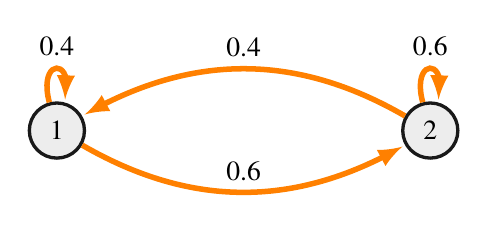
\begin{tikzpicture}[
roundnode/.style={circle, draw=black!90, fill=black!7, very thick, minimum size=7mm},
]
%Nodes
\node[roundnode]        (Computer_Science)        {1};
\node[roundnode]        (Mathematics)       [right=4cm of Computer_Science] {2};
%Lines
 \draw[every loop,
        auto=right,
        line width=0.7mm,
        >=latex,
        draw=orange,
        fill=orange]
            (Computer_Science) edge[bend right, auto=left]  node {0.6} (Mathematics)
            (Mathematics) edge[bend right, auto=right] node {0.4} (Computer_Science)
            (Computer_Science) edge[loop above]             node {0.4} (Computer_Science)
            (Mathematics) edge[loop above]             node {0.6} (Mathematics);
\end{tikzpicture}
    \par{Markov Diagram}
\end{figure}
\par Given that her initial state is $X_0=1$ ($\because$ she studies CS on Monday(n=0)).\\ The $\pr{X_{n+t}=j \, |\, X_{n}=i}$ is given by the $(i,j)$th position of $P^{\,t}$. Therefore $\pr{X_{2}=1 | X_{0}=1}$ ($\because$ n=2 for Wednesday) is the $(1,1)$th position of $P^2$.
\begin{align}
    P^2=\begin{bmatrix}
0.4 & 0.6 \\
0.4 & 0.6
\end{bmatrix}\times
\begin{bmatrix}
0.4 & 0.6 \\
0.4 & 0.6 
\end{bmatrix}=
\begin{bmatrix}
0.4 & 0.6 \\
0.4 & 0.6 
\end{bmatrix}
\end{align}
\par $\therefore$ The probability she studies computer science on Wednesday is $P_{1\,1}^{\,2} = 0.4$.\\
(\textbf{Ans: Option (C)})

%
\item The lifetime of a component of a certain type is a random variable whose probability density function is exponentially distributed with parameter 2. For a randomly picked component of this type, what is the probability that its lifetime exceeds the expected lifetime (rounded to 2 decimal places) ?
%
\solution

Given, The lifetime of a component $X \sim \exp(2)$. The probability density function (PDF) of random variable X is given by:
\begin{align}
  f_X(x) = 
  \begin{cases}
     \lambda e^{-\lambda x}, & \text{for } 0<x<\infty\\
    0, & \text{otherwise } 
  \end{cases}
\end{align}
where: the parameter $\lambda = 2$.
Since, the PDF of the random variable is exponentially distributed,
Expected Lifetime = $E(X)=\frac{1}{\lambda}=\frac{1}{2}=0.5$
\begin{align}
\pr{X > E(X) } &= \int_{\frac{1}{\lambda}}^{\infty} \lambda e^{-\lambda x} \,dx\\
&= -e^{-\lambda x} \Bigr|_{\frac{1}{\lambda}}^{\infty} \\
&= \lim_{x \to \infty} (-e^{-\lambda x}) - (-e^{-\lambda\times \frac{1}{\lambda}})\\
&= \frac{1}{e}\\
&= 0.36787944117
\end{align}
%
\item A die is rolled three times The probability that exactly one odd number turns up among the three outcomes is?
%
\solution

     Let \textbf{X} be the random variable such that it  represents  number of times an odd number appeared .\\
      Let \textbf{Y} be the random variable such that it  represents  number of times an even number appeared .\\
     Let \textbf{C}  be the event that exactly one odd number appears in 3 outcomes.\\
   $\Pr\brak{X=m,Y=n}=\binom{m+n}{m}\times\brak{\frac{1}{2}}^{m+n}$
   

    \begin{align}
    \centering
    \tag{1}
  \Pr\brak{\textbf{C}}&=\Pr\brak{X=1,Y=2}\label{cs1999-1:eq1}\\
  \tag{2}
  \Pr\brak{X=1,Y=2}&=\binom{1+2}{1}\times\brak{\frac{1}{2}}^{1+2}\label{cs1999-1:eq2}\\
  \tag{3}
  \Pr\brak{X=1,Y=2}&=\binom{3}{1}\times\brak{\frac{1}{2}}^{3}\label{cs1999-1:eq3}\\
  \tag{4}
  \Pr\brak{X=1,Y=2}&=\frac{3}{8}\label{cs1999-1:eq4}\\
  \tag{5}
 \Pr\brak{\textbf{C}}&=\Pr\brak{X=1,Y=2}\label{cs1999-1:eq5}\\
  \tag{6}
  \Pr\brak{\textbf{C}}&=\frac{3}{8}\label{cs1999-1:eq6}
   \end{align}

%
\item Four fair six-sided dice are rolled.The probability that sum of results being 22 is $\frac{X}{1296}$.the value of X is
%
\solution



Let X and Y be a random variable which takes values from set A and B respectively.We want to calculate Pr(X+Y=16)
\begin{equation}
  p_X(n)=\begin{cases}
    \dfrac{1}{4}, & \text{if } 2\leq n\leq 5.\\
    0, & \text{otherwise}.
  \end{cases}
\end{equation}
\begin{equation}
  p_Y(n)=\begin{cases}
    \dfrac{1}{5}, & \text{if } 11\leq n\leq 15.\\
    0, & \text{otherwise}.
  \end{cases}
\end{equation}
\begin{align}
&p_z(n) = \Pr(X+Y = n) = \Pr(Y=n-X)\\
&p_z(n) = \sum_k p_x(k)p_y(n-k) = p_x(n) * p_y(n)\\
&p_z(n) = \frac{1}{4} \sum_{k=2}^5 p_y(n-k)=\frac{1}{4}\sum_{k=n-5}^{n-2} p_y(k)
\end{align}
\begin{equation}
  p_z(n)=\begin{cases}
  &0 , n < 13\\
  &\dfrac{1}{20}\times (n-12) ,13 \leq n < 16\vspace{0.2cm}\\
  &\dfrac{1}{20} \times 4 , 16 \leq n \leq 17\vspace{0.2cm}\\
  &\dfrac{21-n}{20} , 18 \leq n \leq 20\vspace{0.2cm}\\
  & 0 ,n > 20
  \end{cases}
\end{equation}
\begin{align}
\therefore p_z(16) = \frac{1}{5}
\end{align}
\begin{figure}[h]
    \centering
    \includegraphics[width=\columnwidth]{solutions/cs/2015/3/figures/assignment4_plot2.png}
\end{figure}
\begin{figure}[h]
    \centering
    \includegraphics[width=\columnwidth]{solutions/cs/2015/3/figures/assignment4_plot1.png}
\end{figure}


%
\item A box contains two coins,one of which is fair and the other is two headed.One coin is choosen at random and tossed twice.If two heads appear,then  the probability that the choosen coin is two headed is?
%
\solution
\input{solutions/ma/1999/1.29.tex}
%
\item Cars arrive at a service station according to Poisson's distribution with a mean rate of 5 per hour.The service time per car is exponential with a mean of 10 minutes.At a steady state,the average waiting time in the queue is 
%
\solution
This problem can be solved using Queuing theory.But first we have to understand queuing theory.
\begin{itemize}
\item In queuing theory we try to determine what happens when people join in queue.
\item\textbf{Parameters for measuring Queuing performance}
\begin{enumerate}
    \item $\lambda$ = Average arrival time
    \item $\mu$ = Average service time
    \item $\rho$ = Utilization factor
    \item $L_q$ = Average number in the queue
    \item $L$ = Average number in the system
    \item $W_q$ = Average waiting time
    \item $W$ = Average time in the system
    \item $P_n$ = Steady state probability of exactly n customers in the system
\end{enumerate}
\item Typically most of the times arrivals follow poisson distribution and services follow exponential distributions.
\item The given question only has one queue so we can conclude that it is a single server model and there is no limit for number of cars in the queue so we can say that it is "\textbf{M/M/1:/$\infty$/$\infty$/FIFO}" by kendall's notation (or) usually "\textbf{M/M/1}" 
\item Here '\textbf{M}' indicates the memory less property of the model first \textbf{M} is for arrival and second one for service and 1 is the number of servers in the model and '$\infty$' indicates the limit of the queue and second '$\infty$' represent population and '\textbf{FIFO}' represents First-In First-Out service.
\item \textbf{NOTE:} In cases where there is no limit in the queue we only take the cases where $\frac{\lambda}{\mu}<1$. Otherwise there could be customers who will not get their service. \newline The memory less property allows us to assume that one event can take place in a small interval of time. The event could be either a arrival or a service.
\item\textbf{Deriving formulas :}
 For the time interval($t,t+h$), where $h \to 0$
\begin{align}
    \Pr{(\text{1 arrival})}&=\lambda h\\
    \Pr{(\text{1 service})}&=\mu h\\
    \Pr{(\text{no arrival})}&=1-\lambda h\\
    \Pr{(\text{no service})}&=1-\mu h
\end{align}
\begin{multline}
    P_{n}(t+h)=P_{n-1}(t)\times\Pr{(\text{1 arrival})}\times\Pr{(\text{no service})}\\
    +P_{n+1}(t)\times\Pr{(\text{no arrival})}\times\Pr{(\text{1 service})}\\
    +P_n(t)\times\Pr{(\text{no arrival})}\times\Pr{(\text{no service})}\label{me2011-19:eq:eq1}
\end{multline}
\begin{multline}
    \implies P_{n}(t+h)=P_{n-1}(t)(\lambda h)(1-\mu h)\\
    +P_{n+1}(t)(\mu h)(1- \lambda h)\\
    +P_n(t)(1-\lambda h)(1-\mu h)
\end{multline}
Now, Neglecting higher order terms of $h$.
\begin{multline}
    \implies P_{n}(t+h)=P_{n-1}\lambda h+P_{n+1}\mu h\\
    +P_n(t)(1-\lambda h-\mu h)
\end{multline}
\begin{multline}
    \implies \frac{P_n(t+h)-P_n(t)}{h}=P_{n-1}(t)\lambda+P_{n+1}(t)\mu\\
    -P_n(t)(\lambda+\mu)
\end{multline}
At steady state, $P_n(t+h)=P_n(t)$
\begin{align}
    \implies\lambda P_{n-1}+\mu P_{n+1}&=(\lambda+\mu)P_n\label{me2011-19:eq:res1}
\end{align}
Now, calculating $P_0(t+h)$ using \eqref{me2011-19:eq:eq1}
\begin{multline}
    P_0(t+h)=P_1(t)(1-\lambda h)(\mu h)\\
    +P_0(t)(1-\lambda h)
\end{multline}
Again, Neglecting higher order terms of $h$
\begin{multline}
    \implies P_0(t+h)=P_1(t)(\mu h)\\
    +P_0(t)(1-\lambda h)
\end{multline}
\begin{align}
    \implies\frac{P_0(t+h)-P_0(t)}{h}&=P_1(\mu)-P_0(\lambda)
\end{align}
At steady state, $P_0(t+h)=P_0(t)$
\begin{align}
    \implies \mu P_1&=\lambda P_0\label{me2011-19:eq:eq2}\\
    \implies P_1&=\brak{\frac{\lambda}{\mu}}P_0\label{me2011-19:eq:res2}
\end{align}
Using \eqref{me2011-19:eq:res1} by substituting $n=1$
\begin{align}
    \lambda P_0+\mu P_2&=(\lambda+\mu)P_1\\
    \implies \lambda P_0+\mu P_2&=\lambda P_1+\mu P_1
\end{align}
from \eqref{me2011-19:eq:eq2} and \eqref{me2011-19:eq:res2}
\begin{align}
    \implies\lambda P_0+\mu P_2&=\lambda P_1+\lambda P_0\\
    \implies P_2&=\brak{\frac{\lambda}{\mu}}P_1\\
    \implies P_2&=\brak{\frac{\lambda}{\mu}}^2P_0\label{me2011-19:eq:eq3}
\end{align}
We assume $\frac{\lambda}{\mu}=\rho$ and generalize $P_n$ by \eqref{me2011-19:eq:res2} and \eqref{me2011-19:eq:eq3}
\begin{align}
  P_n&=\brak{\frac{\lambda}{\mu}}^nP_0\\
  \implies P_n&=\rho^nP_0\label{me2011-19:eq:res3}
\end{align}
We know that sum of all probabilities equal to 1
\begin{align}
    \sum_{i=1}^{\infty}P_i&=1\\
    \implies P_0+P_1+P_2+....&=1
\end{align}
Using \eqref{me2011-19:eq:res3}
\begin{align}
    \implies P_0+\rho P_0+\rho^2P_0+....&=1\\
    \implies P_0\brak{1+\rho+\rho^2+...}&=1\\
    \implies P_0\brak{\frac{1}{1-\rho}}&=1\\
    \implies P_0&=1-\rho\label{me2011-19:eq:res4}\\
    \therefore P_n=\rho^n(1-\rho)
\end{align}
The number of people in the system ($L_s$) is the expected value
\begin{align}
    L_s&=\sum_{i=0}^{\infty}iP_i\\
    \implies L_s&=\sum_{i=0}^{\infty}i\rho^iP_0\\
    \implies L_s&=\rho P_0\sum_{i=0}^{\infty}i\rho^{i-1}\\
    \implies L_s&=\rho P_0\sum_{i=0}^{\infty}\frac{d}{d\rho}\brak{\rho^i}\\
    \implies L_s&=\rho P_0\frac{d}{d\rho}\sum_{i=0}^{\infty}\rho^i\\
    \implies L_s&=\rho P_0\frac{d}{d\rho}\brak{\frac{1}{1-\rho}}\\
    \implies L_s&=\rho P_0\frac{1}{(1-\rho)^2}
\end{align}
By using \eqref{me2011-19:eq:res4}
\begin{align}
    \implies L_s&=\rho(1-\rho)\frac{1}{(1-\rho)^2}\\
    \implies L_s&=\frac{\rho}{1-\rho}
\end{align}
We can also say that the number of people beign served is $\rho$
\begin{align}
    \therefore L_s&=L_q+\text{people beign served}\\
    \implies L_s&=L_q+\rho\\
    \implies L_q&=L_s-\rho\\
    \implies L_q&=\frac{\rho}{1-\rho}-\rho\\
    \implies L_q&=\frac{\rho^2}{1-\rho}
\end{align}
\newpage
The relation between $L_s$ and $W_s$ and $L_q$ and $W_q$ are the Little's equation and they are related as
\begin{align}
    L_s&=\lambda W_s\\
    L_q&=\lambda W_q
\end{align}
\end{itemize}
\section{Solution}
From the question given,
\begin{align}
    \lambda &=5\text{hr}^{-1}\\
    \mu&=\frac{1}{10}\text{min}^{-1} =6\text{hr}^{-1}
    \end{align}
Therefore,
\begin{align}
    \text{Utilization rate}(\rho)&=\frac{\lambda}{\mu}=\frac{5}{6}
    \end{align}
Average number (or) length in queue be $L_q$
    \begin{align}
    L_q&=\frac{\rho^2}{1-\rho}\\
    &=\frac{\brak{\frac{5}{6}}^2}{1-\frac{5}{6}}\\
    &=\frac{25}{6}
    \end{align}
Let the Average waiting time in queue be $W_q$
    \begin{align}
    W_q&=\frac{L_q}{\lambda}\\
    &=\frac{\frac{25}{6}}{5}\\
    &=\frac{5}{6}\text{hr}=50\text{min}
\end{align}
The average waiting time in the queue is 50 min.
\newpage
\begin{table}[h!]
\centering
\resizebox{\columnwidth}{!}
{
    \begin{tabular}{|c|c|}
    \hline
    Parameter & Value \\
    \hline
    $\lambda$ & $5$hr$^{-1}$\\
    \hline
    $\mu$ & $6$hr$^{-1}$\\
    \hline
    $\text{Utilization rate}\brak{\rho}=\frac{\lambda}{\mu}$ & $\frac{5}{6}$\\[1ex]
    \hline
    $\text{Length in queue}\brak{L_q}=\frac{\rho^2}{1-\rho}$ & $\frac{25}{6}$\\[1ex]
    \hline
    $\text{Waiting time in queue}\brak{W_q}=\frac{L_q}{\lambda}$ & $\frac{5}{6}$hr\\[1ex]
    \hline     
    \end{tabular}
}
    \caption{Parameters of the given question and values.}
    \label{me2011-19:TABLE-1}
\end{table}
%
\item Two dice are thrown simultaneously. The probability that at least one of them will have 6 facing up is
\begin{enumerate}[label={\Alph*)}]
    \item 1/36
    \item 1/3
    \item 25/36
    \item 11/36
\end{enumerate}
%
\solution
 \begin{table}[ht]
  \centering
  \begin{tabular}{|c|c|}
        \hline
         Number of dices & \(n\) = 2\\
         \hline
         The total no. of outcomes & 36\\ 
        \hline
         Probability of 6 facing-up & \(p\) = 1/6 \\
        \hline
         Probability of 6 'NOT' facing-up & \(q\) = 5/6 \\
        \hline
         Number of sixes in the outcome & \(X\) \\ 
        \hline
    \end{tabular}
\end{table}
Probability of at least one six facing up
    \begin{align}
         & = {Pr(X = 1)} + {Pr(X = 2)} \\
         & = {^2 C _1}{p}{q} + {^2 C _2}{p^2}{q^0}\\
         & = {^2 C _1} \left( {\frac{1}{6}}\right) \left( {\frac{5}{6}}\right) + {^2 C _2} \left(\frac{1}{6}\right) ^2\\ 
         & = 2 \left(\frac{5}{36}\right) + \frac{1}{36}\\
         & = \frac{11}{36}
    \end{align}

%
\item Suppose we uniformly and randomly select a permutation from the 20\(!\) permutations of 1,2,3,\ldots,20. What is the probability that 2 appears at an earlier position than any other even number in the selected permutation.
\begin{enumerate}[label=(\Alph*)]
    \item \(\displaystyle\frac{1}{2}\)\newline
    \item \(\displaystyle\frac{1}{10}\)\newline
    \item \(\displaystyle\frac{9!}{20!}\)\newline
    \item \normalsize{None of the above.}\newline
\end{enumerate}

%
\solution
 \begin{table}[ht]
  \centering
  \begin{tabular}{|c|c|}
        \hline
         Number of dices & \(n\) = 2\\
         \hline
         The total no. of outcomes & 36\\ 
        \hline
         Probability of 6 facing-up & \(p\) = 1/6 \\
        \hline
         Probability of 6 'NOT' facing-up & \(q\) = 5/6 \\
        \hline
         Number of sixes in the outcome & \(X\) \\ 
        \hline
    \end{tabular}
\end{table}
Probability of at least one six facing up
    \begin{align}
         & = {Pr(X = 1)} + {Pr(X = 2)} \\
         & = {^2 C _1}{p}{q} + {^2 C _2}{p^2}{q^0}\\
         & = {^2 C _1} \left( {\frac{1}{6}}\right) \left( {\frac{5}{6}}\right) + {^2 C _2} \left(\frac{1}{6}\right) ^2\\ 
         & = 2 \left(\frac{5}{36}\right) + \frac{1}{36}\\
         & = \frac{11}{36}
    \end{align}

%
\item  Consider a single machine workstation to which jobs arrive according to a
Poisson distribution with a mean arrival rate of 12 jobs/hour. The process
time of the workstation is exponentially distributed with a mean of 4
minutes. The expected number of jobs at the workstation at any given
point of time is \ldots (\textit{round off to the nearest integer}).
%
\solution
In a Poisson process,
 \begin{align}
          \pr{X=x}&= e^{-\lambda \Delta t} \frac{(\lambda \Delta t)^{x}}{x\,!}
 \end{align}
If $\Delta t \rightarrow 0$ then probability of having only one Poisson job is  
  \begin{align}
         \pr{X=1}=\lambda \Delta t \label{me2021-42:singlejob-condition}
 \end{align}
 Some assumptions:\\
 In time interval $\Delta t$,
 \begin{itemize}
     \item Exactly one job is arrived  
     \item or Exactly one job is completed
     \item or Nothing happens
 \end{itemize}
Assumptions seem quite reasonable as $\Delta t$ is very small then the probability of occurrence of more than one poisson job is very low.\\
 For job arrival,
 \begin{itemize}
 \item It is distributed according to Poisson distribution.
     \item Its
 Rate parameter $\lambda $=12 jobs/hour.
 \item Using \eqref{me2021-42:singlejob-condition},Probability that a single job arrives in a small interval $\Delta t=\lambda\Delta t$.
 \end{itemize}
 For Job completions,
 \begin{itemize}
     \item  Job completion time is distributed exponentially with mean of 4 minutes 
     \item Then we can assume that no. of job completions are distributed as Poisson distribution with rate parameter $\mu$ = 15 jobs/hour
     \item Once again using \eqref{me2021-42:singlejob-condition},
 Probability that a single job will be completed in a small interval $\Delta t=\mu \Delta t$
 \end{itemize}
 Some notations,
 \begin{table}[h]
\begin{tabular}{|c|p{6cm}|}
\hline
\textbf{Parameter} & \textbf{Definition}                               \\ \hline
$\lambda$          & Poisson rate parameter for the arrival of jobs    \\ \hline
$\mu$              & Poisson rate parameter for the completion of jobs \\ \hline
$\lambda \Delta t$ & Probability that a single job arrives in a small interval $\Delta t$\\\hline 
$\mu \Delta t$ & Probability that a single job will be completed in a small interval $\Delta t$\\\hline 
$P_j(t)$             & probability of having j jobs at workstation at time t \\\hline
$\pi_j$            & steady probability of having j jobs at workstation\\\hline
\end{tabular}
\caption{Parameters and their definitions used in the problem}
\label{me2021-42:tab:parameters}
\end{table}
 \begin{itemize}
     \item  Initial no.of jobs at workstation is 0.
     \item Let $P_{j}(t)$ denote the probability of having $j$ jobs waiting at the workstation at the time $t$ for this initial case.
     \item After a long time,probability of having  j jobs becomes steady.
     \item Let us denote steady state probability of having j jobs as $\pi_j$.
 \end{itemize}
 Condition which ensures that steady state is reached is
 \begin{align}
     \diff{P_j(t)}{t}&=0\\
     \lim_{\Delta t\rightarrow 0}\dfrac{P_j(t+\Delta t)-P_j (t)}{\Delta t}&=0\label{me2021-42:steady-condition}
 \end{align}
  We can reach a state of $j$ jobs at time $t+\Delta t$ from
  \begin{itemize}
      \item A state of $j-1$ jobs at time $t$ with a new job arriving in the next $\Delta t$
      \item A state of $j+1$ jobs at time $t$ with a job completing in the next $\Delta t$
      \item A state of $j$ jobs at time $t$ and nothing happening in the next $\Delta t$
  \end{itemize}
 Assuming time  $t$ is long enough for the occurrence of steady state.The above relations can be shown in probability equations as:  
 \begin{align}
     P_j(t+\Delta t)&=P_{j-1}(t)\lambda\Delta t+ P_{j+1}(t)\mu \Delta t \nonumber\\&+P_j (t) (1-\lambda\Delta t -\mu \Delta t)\\
     \dfrac{P_j(t+\Delta t)-P_j (t)}{\Delta t}&= P_{j-1}(t)\lambda +P_{j+1}(t)\mu\nonumber\\& - P_j(t)\lambda -P_j(t)\mu
\end{align}
Using \eqref{me2021-42:steady-condition} we get,
\begin{align}
     \implies P_{j-1}(t)\lambda +P_{j+1}(t)\mu&=P_j(t)\lambda +P_j(t)\mu \\
     \pi_{j-1}\lambda +\pi_{j+1}\mu&=\pi_j\lambda +\pi_j\mu\label{me2021-42:recursive} 
 \end{align}
 Note that the above equations are  for $j \geq 1$. \\
 For j=0 jobs at time $t+\Delta t$ we can reach it from j=1 job at time $t$ with a job completion in the next $\Delta t$ or else stay at j=0 at time $t$ and do nothing the next $\Delta t$
\begin{align}
    P_0(t+\Delta t)&=P_1(t)\mu \Delta t+\nonumber\\&~~~~P_0(t)(1-\lambda \Delta t)\\
    \dfrac{P_0(t+\Delta t)-P_0(t)}{\Delta t}&=P_1(t) \mu \Delta t-P_0(t)\lambda \Delta t
\end{align}
Once again using \eqref{me2021-42:steady-condition},we will get,
\begin{align}
    P_0(t)\lambda \Delta t&= P_1(t) \mu \Delta t\\
    P_0(t)\lambda&=P_1(t) \mu \\
    \pi_0 \lambda&=\pi_1\mu\label{me2021-42:base}
\end{align}
Solving \eqref{me2021-42:base} and \eqref{me2021-42:recursive} with appropriate j one by one,we will get $P_j$ in terms of $P_0$ as
\begin{equation}
    P_j=\brak{\dfrac{\lambda}{\mu}}^jP_0 
\end{equation}
consider $\rho = \dfrac{\lambda}{\mu}$.
\begin{table}[h]
\begin{tabular}{|c|p{6cm}|}
\hline
\textbf{Parameter} & \textbf{Definition}                               \\ \hline
$E(j)$             & Expected no. of jobs at workstation \\ \hline
$\rho$             & $\dfrac{\lambda}{\mu}$\\\hline
\end{tabular}
\caption{Parameters and their definitions used in the problem}
\label{me2021-42:tab:parameters}
\end{table}
\begin{equation}
    P_j=\rho^j P_0 \label{me2021-42:solution}
\end{equation}
We can prove that \eqref{me2021-42:solution} is indeed the solution of recursion equation \eqref{me2021-42:recursive} by using mathematical induction.\\
Assuming $\rho<1$,let us calculate $P_0$ in terms of $\rho$
\begin{align}
    \sum_{j=0}^{\infty}P_j&=1\\
    \sum_{j=0}^{\infty}\rho^j P_0 &=1\\
    \dfrac{P_0}{1-\rho}&=1\\
    P_0&=1-\rho
\end{align}
This yields,\\
\begin{equation}
    P_j=\rho^j(1-\rho)
\end{equation}
Let us calculate expected value of jobs waiting at workstation.
\begin{align}
    E(j)&=\sum_{j=0}^{\infty}jP_j\\
    E(j)&=(1-\rho)\sum_{j=0}^{\infty}j\rho^j\label{me2021-42:first}\\
    \rho E(j)&=(1-\rho)\sum_{j=0}^{\infty}j\rho^{j+1}\\
    \rho E(j)&=(1-\rho)\sum_{j=1}^{\infty}(j-1)\rho^{j}\label{me2021-42:second}
\end{align}
Subtracting \eqref{me2021-42:second} from \eqref{me2021-42:first}.we get,
\begin{align}
    (1-\rho)E(j)&=(1-\rho)\sum_{j=1}^{\infty}\rho^j\\
    E(j)&=\sum_{j=1}^{\infty}\rho^j\\
    E(j)&=\dfrac{\rho}{1-\rho}\label{me2021-42:expect}
\end{align}
In our case $\rho=\dfrac{\lambda}{\mu}=\dfrac{12}{15}=\dfrac{4}{5}$.\\\\Substituting it in the \eqref{me2021-42:expect} we get,\\
\begin{equation}
    E(j)=4
\end{equation}
$\therefore$ Expected no.of jobs at workstation is 4.

%
\item Consider a binomial random variable X. If \textbf{$X_1,X_2,...,X_n$} are independent and identically distributed samples from the distribution of \textbf{X} with sum Y=$\Sigma_{i=1}^n X_i$, then the distribution of \textbf{Y} as $n\rightarrow \infty$ can be approximated as
\begin{enumerate}
    \item Exponential
    \item Bernoulli 
    \item Binomial
    \item Normal
\end{enumerate}
%
\solution
Given a binomial random variable \textbf{X} 
\begin{align}
\Rightarrow X \sim B\brak{r,p}
\end{align}
also given that $X_1,X_2,...,X_n$ are independent and identically distributed samples 
\begin{align}
    \Rightarrow X_1=X_2=...=X_n=X \sim B\brak{r,p}
\end{align}
also given that
\begin{align}
Y&=\displaystyle\sum_{i=1}^n X_i
\end{align}
We know that the characteristic equation of binomial trials with n elements is \begin{align}
    \phi_X\brak{t}&={\brak{1-p+p e^{it}}}^n
\end{align}
consider two sets of Bernoulli trials containing $r_1 \& r_2$ elements respectively where both trials have the same probability 'p'$\brak{X\sim B\brak{r_1,p},Y\sim\brak{r_2,p}}$. Now considering both as a whole set
\begin{align}
B\brak{r_1,p}+B\brak{r_2,p}&=\Phi_{X+Y}\brak{t}\\
&=\Phi_X\brak{t}\times \Phi_Y\brak{t}\nonumber\\
&={\brak{1-p+p e^{it}}}^{r_1}\nonumber\\
&\hspace*{1cm}\times {\brak{1-p+p e^{it}}}^{r_2}\\
&={\brak{1-p+p e^{it}}}^{r_1+r_2}\\
&=B\brak{r_1+r_2,p}\nonumber\\
\therefore B\brak{r_1,p}+B\brak{r_2,p}&=B\brak{r_1+r_2,p}
\end{align}
using this recursively we get
\begin{align}
    Y&=B\brak{r n,p}
\end{align}
$\Rightarrow$ using standard formulae
\begin{align}
\text{mean of Y } \mu_Y&=nrp \nonumber\\
\text{and variance } \sigma^2_Y&=nrp\brak{1-p}
\end{align}
By central limit theorem\brak{CLT}
\begin{align}
    Z_n &= \sqrt{n}\brak{\frac{\frac{Y}{n} - \mu_Y}{\sigma_Y}}\nonumber\\
    &=\frac{Y-n \mu_Y}{\sqrt{n} \sigma_Y}
\end{align}
$\lim_{n \rightarrow \infty} Z_n \sim N\brak{0,1}$ \\
Which is a normal distribution\\
$\therefore$ the correct answer is option D
%
\item Let \(X\) be a continuous random variable denoting the temperature measured. The range of temperature is [0,100] degree Celsius and let probability density function of \(X\) be \(f(x)\)=0.01 for 0 \(\leq X \leq\) 100.\newline
The mean of \(X\) is ?\newline
%
\begin{enumerate}[label=(\Alph*)]
    \item \(2.5\)
    \item \(5.0\)
    \item \(25.0\)
    \item \(50.0\)
\end{enumerate}
%
\solution
Given \(X\) is a continuous random variable.
The probability density function of X is \(f(x)\)

\begin{align}
    f(x) = 
	\begin{cases}
	0.01 &  0 \leq x \leq 100\\ ~\\[-1em]
	0 & \text{otherwise}
	\end{cases}
\end{align}
\begin{flushleft}
Mean of the random variable X is \(\mu\)
\end{flushleft}
\begin{align}
    \mu &= \int\limits_{-\infty}^{\infty} x\,f(x)\,\mathrm{d}x =\displaystyle\int\limits_{0}^{100} x\,(0.01)\,\mathrm{d}x\\\nonumber\\
    &=(0.01)\displaystyle\int\limits_{0}^{100} x\,\mathrm{d}x = (0.01)\;\;\frac{x^2}{2}\bigg\vert_0^{100}\\\nonumber\\
    &=50.0 \text{  degree Celsius}\\\nonumber
\end{align}

%
\item Two die are thrown. What is the probability that sum of numbers on the two dice is eight \\
\begin{enumerate}[label=(\alph*)]
\item $\frac{5}{36}$\\
\item $\frac{5}{18}$ \\
\item$\frac{1}{4}$\\
\item$\frac{1}{3}$
\end{enumerate}
%
%
\solution
Let $X$ be a discrete random variable which denotes the sum obtained on two dice and $X_{1} \in \{1,6\}$ be a discrete random variable denoting the outcome on a single die.
\begin{align}
\pr{X=n}=
\begin{cases}
 0 , &\text{if } n < 1 \\
 \frac{n-1}{36} , &\text{if } 1 \leq n-1 \leq 6\\
 \frac{13-n}{26} , &\text{if } 1 < n-6 \leq 6\\
 0 , &\text{if } n > 12 \label{me2002-1.1:1.0.1}
\end{cases}
\end{align}
\begin{align}
    \text{Required probability}  = \pr{X=8}  \notag 
\end{align}
\begin{align}
  \text{So, from \eqref{me2002-1.1:1.0.1},}  \pr{X=8}= \frac{5}{36} \notag
\end{align}
%
\item A binary symmetric channel $\brak{BSC}$ has a transition probability of $\frac{1}{8}$. If the binary symbol X is such that P $\brak{X = 0}$ = $\frac{9}{10}$ , then the probability of error for an optimum receiver will be 
\begin{enumerate}[]
\begin{multicols}{2}
\setlength\itemsep{0.1em}
\item $\frac{7}{80}$ \label{ec2012-35option A}
\item $\frac{63}{80}$ \label{ec2012-35option B}
\item $\frac{63}{80}$ \label{ec2012-35option C}
\item  $\frac{1}{10}$ \label{ec2012-35option D}
\end{multicols}
\end{enumerate}
%
\solution
Probability of  transition,p is given by
\begin{align}
    p =  \frac{1}{8} \\
    \pr{X = 0} = \frac{9}{10} \\
    \pr{X = 1} = \frac{1}{10}
\end{align}
\begin{center}
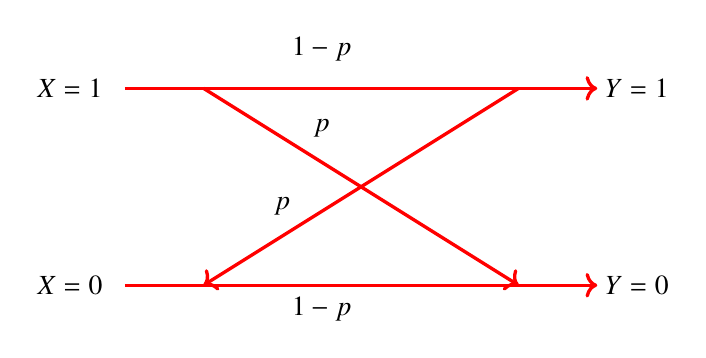
\begin{tikzpicture}
\begin{scope}[red,very thick,->]
    \draw  (0,0) -- (6,0);
   \draw (1,0) -- (5,-2.5);
   \draw (5,0) -- (1,-2.5);
   \draw (0,-2.5) -- (6,-2.5);
\end{scope}
   \node at (-0.7,0) {$\displaystyle X = 1 $};
   \node at (6.5,0)  {$\displaystyle Y = 1$};
   \node at (-0.7,-2.5) {$\displaystyle X = 0$};
   \node at (6.5,-2.5) {$\displaystyle Y = 0$};
   \node at (2.5,0.5) {$\displaystyle 1-p$};
   \node at (2.5,-2.8) {$\displaystyle 1-p$};
   \node at (2.5,-0.5) {$\displaystyle p$};
   \node at (2,-1.5) {$\displaystyle p$};
\end{tikzpicture}
\end{center}
\begin{center}
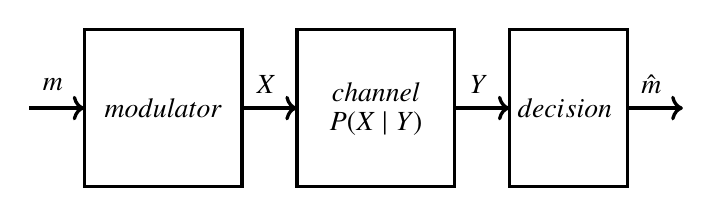
\begin{tikzpicture}
\begin{scope}[black,very thick,->]
         \draw (-0.3,0) rectangle (1.7,2); 
    \draw (2.4,0) rectangle  (4.4,2);
    \draw [->] (1.7,1) -- (2.4,1);
    \draw [->] (4.4,1) -- (5.1,1);
    \draw (5.1,0) rectangle (6.6,2);
    \draw [->] (6.6,1) -- (7.3,1);
    \draw [->] (-1,1) -- (-0.3,1);
\end{scope}
    \node at (1.5,1.5) {$\displaystyle $};
    \node at (1.5,0.5) {$\displaystyle $};
    \node at  (0.7,1)  {$\displaystyle modulator$};
    \node at  (-0.7,1.3)  {$\displaystyle m$};
    \node at  (2,1.3)  {$\displaystyle X$};
    \node at  (4.7,1.3)  {$\displaystyle Y$};
    \node at  (6.9,1.3)  {$\displaystyle \hat{m}$};
    \node at  (5.8,1)  {$\displaystyle decision$};
    \node at  (3.4,1.2)  {$\displaystyle channel$};
    \node at  (3.4,0.8)  {$\displaystyle P(X \mid Y)$};
\end{tikzpicture}
(here $m$ and $X$ can be considered similar)
\end{center}
$\therefore$ Probability of error is defined as 
\begin{align}
    P_e = \pr{\hat{m} \neq m}
\end{align}
Probability of being correct is defined as
\begin{align}
    P_c & = 1 - P_e  \\
        & = 1 - \pr{\hat{m} \neq m} \\
        & = \pr{\hat{m} = m} 
\end{align}
Optimum detector maxmize $P_c$ or equivalently minimize $P_e$ \\ Probability of making correct decision, for a given received y 
\begin{align}
    P_c & = \pr{\hat{m} = m} \\
        & = p(m_i \mid y) p(y) \\
        & = p(x_i \mid y) p(y)
\end{align}
Using Bayes theorem,
\begin{align}
    P_c & = p(y \mid x_i) p(x_i)
\end{align}
To maximize $P_c$ we use \textbf{Maximum a Posterior Detector (MAP)} rule , for a given $Y$
\begin{align}
    \hat{m} \implies m_i \ \ if \ \ \frac{p(y \mid x_i) p(x_i)}{p(y \mid x_j) p(x_j)} \geq 1
\end{align}
Now , when Y = 1 then $\hat{m}$ = 0 if
 
\begin{align}
    \frac{p(y = 1 \mid x = 0) p(x=0)}{p(y =1  \mid x = 1) p(x=1)} \geq 1 \\
\implies  \frac{p(y = 1 \mid x = 0) p(x=0)}{p(y =1  \mid x = 1) p(x=1)} \\
= \frac{\frac{1}{8} \cdot \frac{9}{10}}{\frac{7}{8} \cdot \frac{1}{10}}  \\
= \frac{9}{7} \geq 1
\end{align}
when Y = 0 then $\hat{m}$ = 0 if
\begin{align}
        \frac{p(y = 0 \mid x = 0) p(x=0)}{p(y = 0  \mid x = 1) p(x=1)} \geq 1 \\
\implies  \frac{p(y = 0 \mid x = 0) p(x=0)}{p(y = 0 \mid x = 1) p(x=1)} \\
= \frac{\frac{7}{8} \cdot \frac{9}{10}}{\frac{1}{8} \cdot \frac{1}{10}}  \\
= 63 \geq 1        
\end{align}
In both cases MAP detector suggest that message will be $\hat{m}$ = 0 \\
$\therefore$ probability of error 
\begin{multline}
    P_e  = \pr{\hat{m} \neq 0 \mid X = 0 } \pr{X = 0} \\ + \pr{\hat{m} \neq 1 \mid X = 1} \pr{X = 1} 
\end{multline}
\begin{align}    
    & = 0 + 1 \cdot \frac{1}{10} \\
    & = \frac{1}{10} 
\end{align}
So answer will be \brak{D}
%
\item If a fair coin is tossed four times,what is the probability that two tails and two heads will result?
%
\solution
Given question is a binomial distribution in which no of trails  $n= 4$.
\\Let's assume a trail is succeeded if the coin turns out to be head.Since it is a fair coin probability of success is $p=0.5$
\\Let $X$ be the binomial random variable of this distribution.
So $X \in \{0,1,2,3,4\}$, 0 represents 0 heads, 1 represents 1 head, 2 represents 2 heads, 3 represents 3 heads and 4 represents 4 heads in 4 trails.
\\From binomial distribution,
\begin{align}
\Pr\brak{\textbf{X=r}}&=\comb{n}{r}p^{r}q^{n-r}
\\&=\comb{n}{r}p^{r}\brak{1-p}^{n-r}
\end{align}
Probability of getting two heads and two trails will be,
\begin{align}
\Pr\brak{\textbf{X=2}}&=\comb{4}{2}\times\brak{0.5}^{2}\times\brak{1-0.5}^{2}
   \\ &= 6\times\brak{\frac{1}{4}}\times\brak{\frac{1}{4}}
   \\ &=\frac{3}{8}
   \\ &=0.375
\end{align}
Hence,the required probability is $0.375$.
%
\item Customers arrive at a shop according to Poisson distribution with a mean of 10 customers/hour. The manager notes that no customer arrives for the first 3 minutes after the shop opens. The probability that a customer arrives within the next 3 minutes is

%
\solution
Given, 
mean of 10 customers arrive in a time interval of 60 minutes $\iff$ mean of $\dfrac{t}{6}$ customers arrive in a time interval of t minutes,
Customers arrive according to Poisson distribution with a mean of $\dfrac{t}{6}$ customers/t minutes,
\begin{align}
\therefore \lambda = \frac{t}{6} \label{me/2021/33/a}
\end{align}
Let $X$ denotes the number of customers in first t minutes,$Y$ denotes the number of customers in second t minutes.
according to  poisson distribution,
\begin{align}
\pr{X=x}= e^{-\lambda} \frac{\lambda^{x}}{x\,!} \label{me/2021/33/b}
\end{align}
using \eqref{me/2021/33/a} in \eqref{me/2021/33/b},
\begin{align}
\pr{X=x}= e^{-\frac{t}{6}} \frac{(\frac{t}{6})^{x}}{x\,!} \label{me/2021/33/c}
\end{align}
 the probability that a customer arrives within the next t minutes given that no customer arrives for the first t minutes after the shop opens,which can also be written as,
\begin{align}
\pr{Y\neq 0|X=0}=\frac{\pr{Y\neq 0,X=0}}{\pr{X=0}}
\end{align}
\begin{table}[ht]
\caption{Probability distribution for values of X and Y}
\begin{center}
    \begin{tabular}{|c|c|c|}
    \hline
     & P(X)&P(Y)\\
    \hline
    0& $e^{-\frac{t}{6}}$& $e^{-\frac{t}{6}}$\\
    \hline
    1 & $\frac{t e^{-\frac{t}{6}}}{6}$ & $\frac{t e^{-\frac{t}{6}}}{6}$\\
    \hline
    \end{tabular}
\end{center} 
\end{table}
As the arrival of customers in second t minutes does not depend on the arrival of customers in first t minutes, X and Y are independent,
\begin{align}
\pr{Y\neq 0|X=0}&=\frac{\pr{Y\neq 0}\pr{X=0}}{\pr{X=0}}\\
&=\pr{Y\neq 0}\\
&= 1-\pr{Y=0} 
\end{align}
using \eqref{me/2021/33/c},
\begin{align}
\pr{Y\neq 0|X=0}&=1- e^{-\frac{t}{6}}
\end{align}
we need to find the probability for t=3,the required probability is given by,
\begin{align}
&=1- e^{-\frac{1}{2}}\\
&=0.3935
\end{align}

\end{enumerate}
\end{document}
